\documentclass[10pt,a4paper]{amsbook}

\usepackage{ucs}
\usepackage[utf8x]{inputenc}
\usepackage{amsmath}
\usepackage{amsfonts}
\usepackage{amssymb}
\usepackage{amsthm}
\usepackage[italian]{babel}
\usepackage{fontenc}
\usepackage[all]{xy}
\usepackage{graphicx}
\usepackage{prooftree}

\usepackage{hyperref}
\hypersetup{%
    colorlinks=true, linktocpage=true, pdfstartpage=3, pdfstartview=FitV,%
    breaklinks=true, pdfpagemode=UseNone, pageanchor=true,
    pdfpagemode=UseOutlines, plainpages=false, bookmarksnumbered,
    bookmarksopen=true, bookmarksopenlevel=1, hypertexnames=true,
    pdfhighlight=/O,%hyperfootnotes=true,%nesting=true,%frenchlinks,%
    %urlcolor=webbrown, linkcolor=RoyalBlue, citecolor=webgreen,
    %pagecolor=RoyalBlue,%
    % uncomment the following line if you want to have black links (e.g., for
    % printing)
    %urlcolor=Black, linkcolor=Black, citecolor=Black, pagecolor=Black,%
    pdftitle={Dispense di Logica 2},%
    pdfauthor={},%
    pdfsubject={},%
    pdfkeywords={},%
    pdfcreator={pdfLaTeX},%
    pdfproducer={LaTeX with hyperref and classicthesis}%
}

\usepackage{tikz}
\usetikzlibrary{shapes,arrows}
% Define block styles
\tikzstyle{decision} = [diamond, draw, fill=white, 
    text width=3.5em, text badly centered, node distance=2cm, inner sep=0pt]
\tikzstyle{block} = [rectangle, draw, fill=white, 
    text width=5em, text centered, minimum height=2em]
\tikzstyle{line} = [draw, -latex']
\tikzstyle{noblock}=[rectangle,
    text width=5em, text centered, minimum height=2em]

\newcommand{\roundentry}[1]{*++[o][F-] {#1}} 
\newtheorem{esempio}{Esempio}[chapter]
\newtheorem{oss}{Osservazione}[chapter]
\newtheorem{prop}{Proposizione}[chapter]
\newtheorem{defi}{Definizione}[chapter]
\newtheorem{lem}{Lemma}[chapter]
\newtheorem{thm}{Teorema}[chapter]
\newtheorem{extra}{Esercizio}
\newtheorem{nota}{Nota}
\newtheorem{programmi}{Definizione}[section]
\newtheorem{progabaco}[programmi]{Teorema}
\newtheorem{corol}{Corollario}[chapter]


\newenvironment{mylisting}
{\begin{list}{}{\setlength{\leftmargin}{1em}}\item\bfseries}
{\end{list}}

\newenvironment{mytinylisting}
{\begin{list}{}{\setlength{\leftmargin}{1em}}\item\tiny\bfseries}
{\end{list}}

\title{Dispense di Logica 2}
\author{}
\date{}

\begin{document}

\maketitle

\tableofcontents

\newcommand{\bew}{\mathsf{Bew}}
% per scrivere eqz più velocemente
\newcommand{\eq}[1]{\begin{equation} #1 \end{equation}}
% per fare le parentesi squadrate
\newcommand{\gdnum}[1]{\ulcorner #1 \urcorner}
% per scrivere pi velocemente un'eqz e darle un label
\newcommand{\eqconnome}[2]{\begin{equation} \label{eq:#2} #1 \end{equation}}

\chapter{Macchine di Turing}

\section{Introduzione}
Intuitivamente diciamo che una funzione \`e calcolabile se esiste un insieme
finito di istruzioni che ci dica esattamente cosa dobbiamo fare, senza lasciare
nulla di sottointeso ed ambiguo. Possiamo parlare quindi di una procedura
effettiva (meccanica) proprio perch\`e la sua esecuzione deve dipendere
unicamente dagli input e dalle regole che applico (fattori come il tempo, lo
spazio, il singolo esecutore non devono influire sul risultato) e quindi
possiamo immaginare tale procedura eseguibile da una macchina ipotetica.

Pensiamo ad una macchina come ad un sistema che possiede certe abilit\`a, \`e
quindi in grado di fare certe cose. Ci concentreremo sulle procedure effettive
che potremo scrivere con una certa macchina e che tipo di funzioni potremo
rappresentare.

\section{Definizione di Macchina di Turing}
Il logico inglese Alan Turing nel suo articolo del 1936 era interessato alla
questione di cosa volesse dire calcolabile e descrisse quindi dei dispositivi
astratti conosciuti come Macchine di Turing. Prima di tutto vediamo pi\`u in
dettaglio come Turing descrive una macchina.

Turing stesso paragon\`o una macchina al comportamento di un essere umano che
sta eseguendo un calcolo.  Immaginiamo perci\'o un uomo seduto ad una scrivania
munito di carta e penna: immaginiamo quindi quest'uomo come una testina di
controllo che possa scrivere simboli di un certo alfabeto su di un ipotetico
foglio di carta che noi chiameremo nastro.

Poich\'e non \`e importante il numero di fogli a disposizione dell'uomo,
supporremo la carta come una risorsa infinita: questo si traduce nel fatto che
il nastro su cui la testina di controllo scrive sia infinito in entrambe le
direzioni.

In secondo luogo, l'uomo pu\`o ricordare ed ha memoria finita, quindi dotiamo la
testina di un numero finito di stati di memoria. Infine, la scrittura su di un
pezzo di carta comporta l'avanzamento del processo di scrittura; parallelamente
la scrittura su nastro di un simbolo comporter\`a l'avanzamento verso destra o
verso sinistra della testina medesima.

Dopo queste analogie possiamo riassumere la definizione di Macchina di Turing in
questo modo.

Una macchina di Turing (MdT) \`e definita da un \textsl{insieme di
  regole} che definiscono il comportamento della macchina su un nastro
di input-output (lettura e scrittura). Il nastro pu\`o essere
immaginato come un nastro di lunghezza infinita diviso in quadratini
dette \textsl{celle}. Ogni cella contiene un simbolo $S_i$ di un certo
alfabeto oppure \`e vuota e questo viene rappresentato dal carattere
Blank ($B$). La macchina ha una testina che si sposta lungo il nastro
iniziando dalla cella che contiene il simbolo pi\`u a sinistra e
analizzando una cella alla volta: i simboli devono essere posizionati
in celle vicine e si possono concatenare anche pi\`u input dividendoli
al pi\`u da un carattere B di Blank. I caratteri di Blank si
susseguono anche al di fuori della sequenza di simboli dati in input,
occupando tutta la lunghezza infinita del nastro.  La testina \`e
dotata di un numero finito di stati di memoria $q_i$. Lo stato ha la
funzione di un'etichetta: ad uno stato $q_i$ corrisponde un'operazione
se viene letto un simbolo $S_j$ e un'altra operazione se viene letto
il simbolo $B$. Inoltre a seconda dello stato in cui la testina si
trova, sa che simboli ha letto prima.

\begin{figure}[htbp!]
\centering
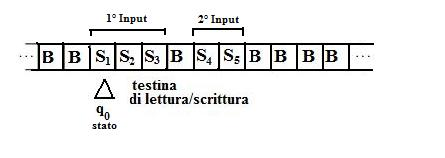
\includegraphics[scale=0.8]{img/Nastro.jpg}
\end{figure}

La macchina legge, scrive oppure cancella i simboli nelle celle del nastro
seguendo l'insieme di regole o quintuple,  che ne definiscono il comportamento.
Tali regole sono di questo tipo:

\vspace{0.3cm}
(\textsl{stato-interno-corrente}, \textsl{simbolo-letto},
\textsl{simbolo-scritto}, \textsl{prossimo-stato-interno}, \textsl{direzione}).
\vspace{0.3cm}

Quindi ad ogni passo, la macchina legge un simbolo sul nastro e in accordo al
suo \textsl{stato interno corrente}:

\begin{enumerate}
\item scrive un simbolo sul nastro
\item decide il suo prossimo stato interno, e decide se spostare la testina a
sinistra (L) o a destra (R) di una posizione.
\end{enumerate}
\vspace{0.5cm}

Diamo di seguito un esempio per queste istruzioni:

\begin{itemize}
\item La quintupla $<q_{i}S_{j}S_{k}Rq_{l}>$ indica che se la macchina
  si trova nello stato interno $q_{i}$ e legge sul nastro il simbolo
  $S_{j}$, allora lo sostituisce con $S_{k}$ e sposta la testina di
  lettura di una cella verso destra passando allo stato $q_{l}$
\item La quintupla $<q_{i}S_{j}S_{k}Lq_{l}>$ indica che se la macchina
  si trova nello stato $q_{i}$ e legge sul nastro il simbolo $S_{j}$,
  allora lo sostituisce con $S_{k}$ e sposta la testina di lettura di
  una cella verso sinistra lungo il nastro passando nello stato
  $q_{l}$.\\ Notiamo che i simboli $S_{j}$ e $S_{k}$ possono
  coincidere (cio\`e non sovrascrive nulla $<q_{i}S_{j}S_{j}Rq_{l}>$),
  cos\`i come $q_{i}$ pu\`o essere uguale a $q_{l}$ (ossia rimane
  nello stesso stato $<q_{i}S_{j}S_{j}Rq_{i}>$).
\item La scrittura del simbolo $B$ di Blank corrisponde a cancellare
  il contenuto di una cella. Ad esempio la quintupla
  $<q_{i}S_{j}BRq_{l}>$ indica che se la macchina si trova nello stato
  $q_{i}$ e legge $S_{j}$, allora cancella il simbolo mettendo il
  blank e sposta la testina di lettura di una cella verso destra
  passando allo stato $q_{l}$.
\end{itemize}

Noi tratteremo, in accordo col fatto che il nostro ``uomo anonim\`o''
non pu\`o scegliere cosa fare ma solo eseguire regole date. Diamo
quindi la seguente definizione:

\begin{defi}
Una Macchina di Turing si dice \underline{deterministica} se dato uno
stato $q_{i}$ e un simbolo $S_{j}$ c'\`e \textsl{al pi\`u} una
quintupla che inizi per $<q_{i},S_{j}...>$ cio\`e la testina
trovandosi in $q_{i}$ e leggendo $S_{j}$ non pu\`o scegliere cosa fare
ma solo eseguire l'unica istruzione corrispondente, \textsl{se c'\`e},
altrimenti significa che la macchina si arresta.
\end{defi}

Inoltre \`e possibile descrivere il nastro in ogni fase della
computazione che fa la macchina. Introduciamo quindi la seguente
definizione:

\begin{defi}
Una \underline{descrizione istantanea} $\alpha$ di una macchina di
Turing $\tau$ \`e un'espressione contenente esattamente un $q_{i}$ (lo
stato), i simboli sul nastro, e la cella in cui si trova la testina al
momento.
\end{defi}

Quindi una descrizione istantanea (ID) $\alpha$ \`e una stringa della
forma $$S_1S_2S_3.....S_{i-1}qS_{i}S_{i+1}......S_{n}$$ dove

\begin{enumerate}
\item q \`e lo stato della macchina di Turing;
\item $S_1S_2S_3.........S_{n}$ \`e la porzione non-blank del nastro;
\item La testina \`e sopra il simbolo i-esimo.
\end{enumerate}
\vspace{0.5cm}

Vediamo ora come una Macchina di Turing effettua i suoi
calcoli. Inizialmente il nastro contiene una sequenza finita di
simboli, detta \textsl{sequenza di ingresso}. Assumiamo che all'inizio
la testina della macchina $\tau$ sia posizionata sulla prima cella di
input, cio\`e sulla prima cella in cui c'\`e un simbolo e diciamo che
$\tau$ si trova nello stato $q_0$. La testina vede un simbolo $S_i$ e
allora parte: cerca tra le quintuple che forniscono le varie
istruzioni quella che comincia per $q_0$ e ha come secondo elemento il
simbolo letto, del tipo $<q_0,S_i..>$. A questo punto vede quale
istruzione deve eseguire (se sovrascrivere un altro simbolo o se
cancellare), in quale direzione andare e in quale stato portarsi, e
cos\`i via. Se non c'\`e una tale quintupla, la macchina si arresta.

Osserviamo che Turing propose l'idea di tale macchina che fosse capace
di eseguire ogni tipo di calcolo su numeri e simboli. Noi per
semplicit\`a ci riconduciamo a calcoli su numeri naturali e vedremo
che ci possiamo ridurre a considerare un alfabeto costituito
unicamente dai simboli 1 e B: $$\Sigma=\left\{1,B\right\}$$ e quindi
con tale alfabeto riusciremo a rappresentare tutti i numeri
naturali. Notiamo infatti che \`e del tutto equivalente considerare un
alfabeto con un simbolo o con n simboli ed i calcolatori, essendo
rappresentazioni di Macchine di Turing ed usando l'alfabeto binario lo
confermano.

Introduciamo ora una notazione che ci permetter\`a di rappresentare i
numeri naturali e quindi gli input da dare alle macchine (compreso lo
0). Per come abbiamo definito la macchina di Turing, risulta che
abbiamo a disposizione l'unico simbolo di input $1$ per rappresentare
ogni naturale o n-upla di naturali che siano nel dominio di una
funzione.

\begin{itemize}
\item preso un numero $n\in {N}$, ad esso associamo un'espressione
$$\overline{n}=1^{n+1}=\underbrace{11...1}_{n+1\ volte}\quad\mbox{.}$$
  Ad esempio $\overline{3}=1111$.
\item in maniera del tutto analoga, a una k-tupla $(n_{1}...n_{k})$ di
  interi non negativi associamo l'espressione
  $\overline{(n_{1}...n_{k})}=\overline{n_{1}}B...B\overline{n_{k}}$. Per
  esempio $$\overline{(1,4,0)}=\overline{1}B\overline{4}B\overline{0}=
  11B11111B1\quad\mbox {.}$$ In questo caso si vede come si procede
  per separare gli input, cio\`e inserendo un $B$.
\end{itemize}

Se invece con questa notazione abbiamo rappresentato nel nastro un
determinato numero indichiamo con $<\overline{n}>$ il numero naturale
da esso rappresentato, ossia $<\overline{n}>=n$.\\ Quindi gli input
che compariranno nella sequenza d'ingresso sono della forma
$$...BB\overline{n_{1}}B\overline{n_{2}}B...B\overline{n_{k}}BB...$$
dove $\overline{n_1},...,\overline{n_k}$ sono i numeri naturali nella
notazione data sopra. Converremo che ogni blocco rappresentante un
argomento \`e separato dagli altri da un solo $B$; in questo modo la
macchina sa dove inizia e termina l'input (se si incontrano due blank
consecutivi, la testina non \`e pi\`u collocata su una delle celle di
input).  La macchina di Turing su un dato input produce un output. Noi
accetteremo output della forma $$...BB\overline{n_r}BB...$$ ove
$\overline{n_r}$ \`e il risultato della computazione. Dunque in output
avremo il nastro contenente un blocco unico contenente tanti $1$
quanti sono necessari per rappresentare il risultato, in modo tale che
anche in questo caso la macchina sa dove comincia e finisce l'output,
e quindi si noti che, una volta calcolata la soluzione, sar\`a
necessario anche cancellare gli input.

\section{Varianti della Macchina di Turing}
Ci sono molteplici varianti della macchina di Turing e seppur non
entrando qui nel dettaglio si pu\`o mostrare che queste hanno la
stessa portata computazionale della macchina di Turing che abbiamo
definito all'inizio.
\begin{itemize}
\item Macchina di Turing Multinastro: invece di esservi un singolo
  nastro, vi sono k nastri indipendenti e k testine di
  lettura-scrittura, una per ogni nastro.
\item Macchina di Turing con movimento arbitrario della testina di
  lettura: si pu\`o modificare la definizione di una macchina di
  Turing in modo che la testina di lettura si possa spostare ogni
  volta di un numero arbitrario di celle
\item Macchina di Turing con nastro bidimensionale: la macchina opera
  su un nastro bidimensionale, e sono permessi spostamenti verso
  sinistra, destra, l'alto, il basso.
\item Macchina di Turing non deterministica: si distingue da quella
  deterministica definita in precedenza per il fatto che, in presenza
  di un determinato stato e di un determinato carattere letto, essa
  permette la presenza di pi\`u quintuple che iniziano con quello
  stato e quel carattere letto.
\end{itemize}


\chapter{Macchine di Turing e Funzioni Calcolabili}

\section{Cosa pu\`o Essere Calcolato}

Le macchine di Turing sono strumenti molto potenti. Per una grande
quantit\`a di problemi di calcolabilit\`a, \`e possibile costruire una
macchina di Turing che sia in grado di eseguire il calcolo
desiderato. Per esempio, abbiamo visto che \`e possibile ideare una
macchina di Turing per eseguire le operazioni aritmetiche di base sui
numeri naturali.

\subsection{Numeri Calcolabili}

Il lavoro originale di Turing trattava i numeri calcolabili. Un numero
si dice Turing-calcolabile se esiste una macchina di Turing che inizia
la computazione su un nastro vuoto e calcola un numero arbitrario, con
una certa approssimazione. Le macchine di Turing possono calcolare
tutti i numeri algebrici (radici di equazioni con coefficienti
algebrici) e molte costanti matematiche, come ad esempio $\textit{e}$
(costante di Nepero) e $\pi$.

\subsection{Funzioni Calcolabili}

Come abbiamo visto in precedenza, le macchine di Turing possono fare
molto pi\`u che calcolare semplici numeri. Tra le altre cose possono
calcolare funzioni numeriche del tipo $f:N^{n}->N$, come ad esempio si
possono scrivere macchine per calcolare la somma, la moltiplicazione,
la sottrazione tra naturali, l'esponenziale, il fattoriale e molte
altre.

Usando una convenzione per rappresentare i simboli di verit\`a TRUE e
FALSE, rappresentando, per esempio, il valore TRUE come una sequenza
di due ``1'' e il valore FALSE come un singolo ``1'', si possono
trattare anche funzioni binarie, ovvero del tipo
$f:N^{n}->\{0,1\}$. Con tali funzioni \`e possibile calcolare la
funzione caratteristica di un predicato. E', inoltre, possibile
combinare i risultati di tali funzioni con gli usuali operatori
booleani: AND, NOT, OR e in aggiunta IF-THEN-ELSE.

Difatti, le funzioni Turing-calcolabili coincidono con le funzioni
ricorsive, di cui tratteremo pi\`u avanti.

\subsection{Macchina di Turing Universale}

Il pi\`u importante e suggestivo risultato del lavoro di Turing
riguarda il fatto che, per come sono state definite le macchine di
Turing, \`e possibile definire la \textit{Macchina di Turing
  Universale} (UTM).

In teoria della computazione si dice macchina di Turing Universale
$T_U$ una macchina di Turing capace di simulare le evoluzioni di ogni
macchina di Turing. Tale macchina ha permesso di dare una risposta
negativa al problema della decidibilit\`a posto da David Hilbert nel
1928. Brevemente, il problema posto da Hilbert riguarda la
possibilit\`a o meno di poter definire un metodo matematico o un
processo per decidere tutti i possibili problemi matematici.

Essenzialmente la UTM \`e in grado di simulare il comportamento di
qualunque macchina di Turing (compresa se stessa!). Un modo per
pensare alla UTM potrebbe essere quello di immaginarla come un
interprete di un linguaggio di programmazione. Quando all'interprete
(concretamente \`e esso stesso un programma) viene dato in input un
programma, questo comincia ad eseguire le istruzioni del programma
dato e, quindi, si comporta proprio come se fosse lo stesso programma,
dato in input, ad essere eseguito.

La macchina di Turing Universale richiede in input una coppia di
numeri naturali (n,m), dove il primo \`e un indice che identifica una
specifica macchina di Turing $T_n$ (in grado di computare una data
funzione f). Mentre, il secondo indice rappresenta l'input sul quale
eseguire la macchina $T_n$.

Per poter definire una macchina del tipo descritto, \`e prima
necessario ideare un modo per rappresentare una macchina di Turing sul
nastro della UTM. E' possibile associare in modo effettivo ad ogni
macchina di Turing un numero naturale che la identifichi
univocamente. L'idea \`e quella di avere una funzione, preferibilmente
biunivoca, che mappi l'insieme delle macchine di Turing, diciamo T,
nell'insieme dei numeri naturali $f:T->N$. A tale scopo, tenendo
presente che le macchine di Turnig sono definite da una quintupla, si
pu\`o prima definire una codifica per i singoli elementi di una
quintupla e in seguito per ogni possibile quintupla. Esistono molti
modi possibili per ottenere questa codifica effettiva. Il paragrafo
\ref{codeffettiva} che segue mostra a titolo di esempio una di queste
possibili codifiche.

L'esecuzione della macchina universale $T_U(n,m)$ corrisponde quindi
ad eseguire la macchina $T_n(m)$.

\begin{center}
$T_U(n,m) = T_n(m)$
\end{center}

\vspace{10pt}

La macchina $T_U$ opera con un nastro che inizialmente in una sua
prima sezione contiene la codifica delle istruzioni della macchina
$T_n$ seguita, dopo un demarcatore particolare bene individuabile,
dallo stesso input m.

E' interesante osservare che la macchina di Turing Universale \`e in
grado di simulare anche la propria evoluzione mentre procede a
simulare una qualsiasi macchina $T$.

I computer programmabili sono effettivamente delle macchine di Turing
universali, poich\`e sono in grado di simulare l'esecuzione di ogni
macchina di Turing (se vengono intese come algoritmi che calcolano
funzioni) tramite l'esecuzione di un programma, che pu\`o essere visto
come un processo di calcolo da eseguire.

\subsection{Codifica Effettiva delle Macchine di Turing}\label{codeffettiva}

Di seguito viene riportato un'esempio di codifica effettiva per le
macchine di Turing. Con tale codifica \`e possibile rappresentare una
qualunque macchina di Turing sul nastro della macchina di Turing
universale.\\

Ogni quintupla nella definizione di una macchina sar\`a codificata
come una sequenza di cinque blocchi di ``1'', separati da un singolo
``0''.
\begin{enumerate}
  \item Il primo blocco di ``1'' sar\`a la codifica del numero dello
    stato corrente, usando la convezione sopra definita per la
    rappresentazione dei numeri naturali sul nastro (n+1 ``1''
    rappresentano il numero n).
  \item Il secondo blocco di ``1'' sar\`a la codifica del simbolo
    corrente (simbolo che si trova sotto la testina). La codifica del
    simbolo corrente dipende dall'alfabeto e dalla notazione per i
    caratteri usata.``1''
  \item Il terzo blocco di ``1'' sar\`a la codifica dell'eventuale
    simbolo da scrivere in posizione sul nastro sottostante la
    testina.
  \item Il quarto elemento rappresenter\`a l'azione che deve essere
    eseguita dalla testina, e ci sono tre possibilit\`a: con un blocco
    di un solo ``1'' si rappresanta lo spostamento nullo, con un
    blocco di due ``1'' lo spostamento a sinistra (L) e con tre ``1''
    lo spostamento a destra (R).
  \item Infine, il quinto elemento della tuple rappresenter\`a il
    numero del nuovo stato in cui la macchina si trover\`a dopo
    l'esecuzione dell'azione richiesta, rappresentato anche esso
    mediante la notazione unaria.
\end{enumerate}

Per codicifare, in fine, l'intera macchina, basta semplicemente
scrivere sul nastro tutte le tuple che caratterizzano la macchina,
separate tra loro da un carattere di \textit{Blank}.

Se si utilizza il carattere ``0'' al posto del carattere
\textit{Blank}, si ottiene una sequenza di ``0'' e di ``1''. Tale
sequenza pu\`o essere interpretata come un numero naturale espresso in
rappresetntazione binaria. Se tale numero viene espresso con la
notazione $\overline{n}=1^{n+1}$, risulta effettivamente possibile
dare in input alla macchina di Turing universale una coppia di numeri
naturali espressi secondo questa notazione.


\section{Cosa non pu\`o Essere Calcolato}
Un altro sorprendente risultato presentato dall'articolo di Turing del
1936 riguarda l'esistenza di problemi ben definiti che non possono
essere risolti da nessuna procedura computazionale. Se questi problemi
sono formulati come formule, possiamo riferirci a queste funzioni come
funzioni non calcolabili; se questi problemi vengono espressi come
predicati, si dice problemi indecidibili. Usando il concetto della
macchina astratta di turing, possiamo dire che una funzione non \`e
calcolabile se non esistono macchine di Turing che sono in grado di
calcolare tale funzione.

Per mostrare l'esitenza di funzioni non calcolabili dalle macchine di
Turing bisogna ragionare sulla cardinalit\`a dell'insieme delle
macchine di Turing e confrontarla con la cardinalit\`a dell'insieme
delle funzioni del tipo $f:N->N$ (con uno sforzo minimo ci si pu\`o
portare al caso pi\`u generale di funzioni $f:N^n->N$).

\begin{center}
$F = \{ f | f \textrm{ \`e una funzione del tipo } f:N->N \}.$
\end{center}

\vspace{10pt}

\begin{center}
$T = \{ t | t \textrm{ \`e una macchina di Turing} \}.$
\end{center}

\vspace{10pt}

Poich\`e \`e possibile, come mostrato in precedenza, costruire una
codifica effettiva delle macchine di Turing, cio\`e costruire una
funzione che associ ad ogni TM un numero naturale unico, l'insieme
delle TM \`e enumerabile, ovvero la sua cardinalit\`a \`e pari a $|N|$
(cardinalit\`a dei numeri naturali). Tuttavia, l'insieme di tutte le
funzioni $f:N->N$ \`e dimostrato non essere enumerabile. Per questo
motivo, possiamo concludere che tutte le macchine di Turing sono in
grado di calcolare solo un sottoinsieme di tutte le funzioni
definibili.

Ci sono molti problemi legati ai programmi che si possono dimostrare
non decidibili. Poich\`e le macchine di Turing sono molto semplici se
comparate con i computer come uso pratico, risulta concettualmente
pi\`u facile provare l'impossobilit\`a di alcuni risultati per le
macchine di Turing. Dando un definizione formale di non banale per una
propriet\`a, H.G. Rice riusc\`i, addirittura, a dimostrare il seguente
teorema:

\begin{thm}
Ogni propriet\`a non banale dei programmi \`e indecidibile.
\end{thm}

E' da notare che dimostrando che un problema \`e non decidibile, non
significa che non pu\`o essere deciso solo in alcuni casi, bens\`i che
\`e impossibile costruire una soluzione \textit{per ogni} possibile
input.



%%%%%%%%%%%%%%%%%%%%%%%%%%%%%%%%%%%%%%%%%%%%%%%%%ESEMPI%%%%%%%%%%%%%%%%%%%%%%%%%%%%%%%%%

\chapter{Macchine di Turing: Esempi}


\section{Esempi di Macchine di Turing}
Diamo ora qualche esempio di semplici macchine di Turing.\\

\begin{itemize}
\item Sia $\Sigma=\left\{0,1\right\}$ l'alfabeto di simboli in
  input. \\\underline{Scopo della macchina:} data una stringa di 0 e 1
  scambia le occorrenze di 1 con 0 e viceversa, riposizionandosi sulla
  cella precedente a quella iniziale.\\ \underline{Passi:} leggere i
  simboli sul nastro e ogni volta che si trova 1 si scrive 0 e
  viceversa. Quando la sequenza di 0 e 1 è finita la testina torna
  sulla cella precedente alla prima significativa.\\

Nastro in input:$$...BB100101BB....$$\\

Sequenza di quintuple:
\begin{eqnarray*}
&<q_0,0,1,R,q_0>&\\
&<q_0,1,0,R,q_0>&\mbox{(scambia 0 e 1)}\\
&<q_0,B,B,L,q_1>&\\
&<q_1,0,0,L,q_1>&\\
&<q_1,1,1,L,q_1>&\mbox{(si riposiziona sulla cella precedente alla prima significativa)}\\
\end{eqnarray*}
Quindi la macchina di Turing per la sequenza di ingresso $...BB100101BB....$ esegue la seguente computazione:
\begin{eqnarray*}
&...BBq_0100101BB...\\
&...BB0q_000101BB...\\
&...BB01q_00101BB...\\
&...BB011q_0101BB...\\
&...BB0110q_001BB...\\
&...BB01101q_01BB...\\
&...BB011010q_0BB...\\
&...BB01101q_10BB...\\
&...\\
&...Bq_1B011010BB...\\
\end{eqnarray*}
Notiamo che l'ultima descrizione istantanea \`e tale da essere
terminale. Infatti arrivata a questo punto la macchina si arresta in
quanto nell'insieme di quintuple che regolano il suo comportamento non
c'\`e una quintupla del tipo $<q_1,B....>$.\\
\vspace{0.3 cm} Nastro in output:$$...BB011010BB....$$ Quindi dato
l'output vediamo che tale macchina sostituisce, nella sequenza data in
input, le occorrenze di 1 con 0 e viceversa.\\
\vspace{0.2cm}
Diagramma:
\begin{figure}[hbtp!]
\hspace{3 cm} \entrymodifiers={++[o][F-]} \xymatrix@=40pt{q_{0}
  \ar@(dr,dl)[]^{1|0 \ R} \ar@(ul,ur)[]^{1|0 \ R} \ar@<2pt>[r]^{B|B
    \ L} & q_{1}\ar@(dr,dl) []^{0|0 \ L} \ar@(ul,ur)[]^{1|1 \ L}\\}
\end{figure}

\item Sia $\Sigma=\left\{1,B\right\}$ l'alfabeto di simboli in
  input. \\\underline{Scopo della macchina:} calcolare il successore
  di un numero naturale dato in input ovvero data una sequenza di
  $n+1$ uni, che rappresenta il numero naturale n, aggiunge alla fine
  della sequenza un altro uno($f(x)=x+1$).\\\underline{Passi:} Essendo
  la testina posizionata nella cella con il primo 1 della sequenza si
  sposta fino al primo B a destra della sequenza. Scrive 1 e torna
  alla posizione di partenza.\\ Nastro in input: $x=2$ rappresentato
  da 3 uni $$BBB111BBB$$ Sequenza di quintuple:
\begin{eqnarray*}
&<q_0,1,1,R,q_0>&\mbox{(scorre tutti gli uni della sequenza)}\\
&<q_0,B,1,L,q_1>&\mbox{(sostituisce il primo B trovato a destra della sequenza con un 1)}\\
&<q_1,1,1,L,q_1>&\\
&<q_1,B,B,R,q_{2}>&\mbox{(si riposiziona sulla prima cella significativa del nastro)}\\
\end{eqnarray*}
Quindi la macchina di Turing per la sequenza di ingresso
$...BB111BB....$ esegue la seguente computazione:
\begin{eqnarray*}
&...BBq_0111BB...\\
&...BB1q_011BB...\\
&...BB11q_01BB...\\
&...BB111q_0BB...\\
&...BB11q_011BB...\\
&...\\
&...Bq_0B1111BB\\
\end{eqnarray*}
Nastro in output: $f(2)=3$ rappresentato da 4 uni $$...BB1111BB....$$
Diagramma:
\begin{figure}[hbtp!]
\hspace{3 cm} \entrymodifiers={++[o][F-]} \xymatrix@=40pt{q_{0}
  \ar@(dr,dl)[]^{1|1 \ R} \ar@<2pt>[r]^{B|1 \ L} & q_{1}\ar@(dr,dl)
      []^{1|1 \ L} \ar@<2pt>[r]^{B|B \ R} & q_{2}}\\
\end{figure}
\begin{oss}
Per calcolare il successore, invece di aggiungere un uno alla fine
della sequenza di uni data in input, si poteva aggiungerlo nella cella
precedente alla prima cella significativa del nastro. In tal caso le
quintuple si sarebbero ridotte a due e precisamente:
\begin{eqnarray*}
&<q_0,1,1,L,q_1>&\mbox{(scorre tutti gli uni della sequenza)}\\
&<q_1,B,1,R,q_2>&\mbox{(sostituisce il primo B trovato a destra della sequenza con un 1)}\\
\end{eqnarray*}
\end{oss}
\item Sia $\Sigma=\left\{1,B\right\}$ l'alfabeto di simboli in
  input.\\\underline{Scopo della macchina:} data in input una sequenza
  (anche di pi\`u input basta siano separati al pi\`u da un B) sposta
  tutta la parte significativa del nastro di una cella verso
  destra.\\ \underline{Passi:} cancellare il primo 1 che si trova, poi
  scorrere la parte significativa del nastro fino al primo B e
  sostituirlo con un 1. Se c'\`e un altro input procede
  analogamente.\\ Nastro in input:$$...BB11B1BB....$$ Sequenza di
  quintuple:
\begin{eqnarray*}
&<q_0,1,B,R,q_1>&\mbox{(cancella il primo 1)}\\
&<q_1,1,1,R,q_1>&\mbox{(scorre la sequenza di 1)}\\
&<q_1,B,1,R,q_2>&\mbox{(sostituisce il primo B con un 1, cos\`i sposta il primo blocco)}\\
&<q_2,1,B,R,q_1>&\mbox{(cancella il primo 1 del secondo input e procede come prima)}\\
&<q_2,B,B,L,q_3>&\\
&<q_3,1,1,L,q_3>&\\
&<q_3,B,B,L,q_4>&\\
&<q_4,1,1,L,q_3>&\\
&<q_4,B,B,R,q_5>&\\
&<q_5,B,B,R,q_6>&\mbox{(si riposiziona sulla prima cella significativa del nastro)}\\
\end{eqnarray*}
Quindi la macchina di Turing per la sequenza di ingresso $...BB11B1BB....$ esegue la seguente computazione:
\begin{eqnarray*}
&...BBq_011B1BB...\\
&...BBBq_11B1BB...\\
&...BBB1q_1B1BB...\\
&...BBB11q_21BB...\\
&...BBB11Bq_1BB...\\
&...BBB11B1q_2BB...\\
&...BBB11Bq_31BB...\\
&...BB011q_3B1BB...\\
&...BBB1q_41B1BB...\\
&...BBBq_311B1BB...\\
&...BBq_3B11B1BB...\\
&...Bq_4BB11B1BB...\\
&...BBq_5B11B1BB...\\
&...BBBq_611B1BB...\\
\end{eqnarray*}
Nastro in output: tutta la sequenza \`e stata spostata di una cella
verso destra $$...BBB11B1BB....$$ Diagramma:
\begin{figure}[hbtp!]
\hspace{3 cm} \entrymodifiers={++[o][F-]} \xymatrix@=40pt{q_{0}
  \ar[d]^{1|B \ R}\\ q_{1}\ar@(dr,dl) []^{1|1 \ R} \ar@<2pt>[r]^{B|1
    \ R} & q_{2}\ar@(d,dr)[l]^{1|B \ R} \ar@<2pt>[r]^{B|B \ L} &
  q_{3}\ar@(dr,dl) []^{1|1 \ L}\ar@<2pt>[r]^{B|B \ L } &
  q_{4}\ar@(d,dr)[l]^{1|1 \ L} \ar@<2pt>[r]^{B|B \ R} & q_{5}
  \ar@<2pt>[r]^{B|B \ R} & q_{6}}\\
\end{figure}

\end{itemize}

\section{Alcune operazioni aritmetiche}
Mostriamo ora alcune macchine di Turing pi\`u complesse, in grado di
calcolare alcune operzioni aritmetiche.\\

\begin{esempio}[Sottrazione]
Vogliamo calcolare la differenza di due numeri naturali non
negativi: $$g(x,\ y)=x-y.$$ L'idea \`e quella di cancellare di volta
in volta un 1 all'inizio e un 1 alla fine della sequenza in input
finch\`e uno dei due blocchi non si svuota e aggiunge un 1 per avere
l'output nella forma standard.\newline Notare che nei naturali $x-y$,
con $x<y$, non \`e definita e per questo la nostra macchina di Turing
per la sottrazione potrebbe andare in loop, ossia non fermarsi
mai. Questo \`e esattamente un esempio di funzione semicalcolabile.\\

Definizione della macchina:
\begin{eqnarray*}
&<q_{0},1,B,R,q_{1}>&\mbox{(cancella l'1 pi\`u a sinistra)}\\
&<q_{1},1,1,R,q_{1}>&\\
&<q_{1},B,B,R,q_{2}>&\mbox{(trova il blank che separa i blocchi)}\\
&<q_{2},1,1,R,q_{2}>&\\
&<q_{2},B,B,L,q_{3}>&\mbox{(trova l'estremit\`a destra)}\\
&<q_{3},1,B,L,q_{4}>&\mbox{(cancella l'1 pi\`u a destra)}\\
&<q_{4},1,1,L,q_{5}>&\\
&<q_{4},B,1,L,q_{9}>&\mbox{(se $y$ \`e stato consumato torno sulla prima cella altrimenti continua)}\\
&<q_{5},1,1,L,q_{5}>&\\
&<q_{5},B,B,L,q_{6}>&\mbox{(trova il blank che separa i blocchi)}\\
&<q_{6},1,1,L,q_{7}>&\\
&<q_{6},B,B,R,q_{8}>&\mbox{(se $x$ \`e stato consumato torna all'inizio senn\`o continua)}\\
&<q_{7},1,1,L,q_{7}>&\\
&<q_{7},B,B,R,q_{0}>&\mbox{(trova l'estremit\`a sinistra e torna in $q_{0}$)}\\
&<q_{8},1,1,L,q_{8}>&\\
&<q_{8},B,B,R,q_{8}>&\mbox{(computa un ciclo infinito se $x< y$)}\\
&<q_{9},1,1,L,q_{9}>&\\
&<q_{9},B,B,R,q_{10}>&\mbox{(torno sulla prima cella significativa del nastro)}\\
\end{eqnarray*}

Grafico:
\begin{figure}[hbtp]
\resizebox{\columnwidth}{!}{%
\hspace{0cm} \xymatrix@=40pt{\roundentry{q_{0}} \ar[r]^{1|BR} &
  \roundentry{q_{1}} \ar@(dr,dl)[]^{1|1R} \ar[r]^{B|BR} &
  \roundentry{q_{2}} \ar@(dr,dl)[]^{1|1R} \ar[r]^{B|BL} &
  \roundentry{q_{3}} \ar@(dr,dl)[]^{1|BL} \ar[r]^{1|BL} &
  \roundentry{q_{4}} \ar[r]^{B|1L} \ar[d]^{1|1L} & \roundentry{q_{9}}
  \ar@(dr,dl)[]^{1|1L} \ar[r]^{B|BR} & \roundentry{q_{10}} \\ &&&&
  \roundentry{q_{5}} \ar@(dr,dl)[]^{1|1L} \ar[r]^{B|BL} &
  \roundentry{q_{6}} \ar[r]^{B|BR} \ar[d]^{1|1L} & \roundentry{q_{8}}
  \ar@(dr,dl)[]^{1|1L} \ar@(ru,rd)[]^{B|BR} \\ &&&&&
  \roundentry{q_{7}} \ar@(dr,dl)[]^{1|1L} \ar `l[lllll] ^{B|BR}
             [llllluu] }}
\end{figure}

Diamo ora qualche esempio di computazione e calcoliamo
quindi $$\overline{m_{1}}-\overline{m_{2}}\mbox{,}\quad
\overline{m_{1}}\mbox{,} \overline{m_{2}}\in \mbox{\upshape N.}$$ La
configurazione iniziale con cui la macchina parte \`e:
$$...BBq_{0}1^{m_{1}+1}B1^{m_{2}+1}BB...$$

Ora la testina si trova in $q_{0}$ e legge un 1, quindi deve cancellarlo. Dunque abbiamo:
$m_{1}\geq m_{2}$. Chiamiamo $k=m_{1} - m_{2}$.\\
\begin{eqnarray*}
&...BBBq_{1}1^{m_{1}}B1^{m_{2}+1}BB...&\mbox{(ho cancellato il primo 1)}\\
&...BBB1q_{1}1^{m_{1}-1}B1^{m_{2}+1}BB...&\\
&.........&\\
&...BBB1^{m_{1}}q_{1}B1^{m_{2}+1}BB...&\\
&...BBB1^{m_{1}}Bq_{2}1^{m_{2}+1}BB...&\mbox{(ho trovato la B che separa i blocchi)}\\
&...BBB1^{m_{1}}B1q_{2}1^{m_{2}}BB...&\\
&.........&\\
&...BBB1^{m_{1}}B1^{m_{2}+1}q_{2}BB...&\\
\end{eqnarray*}
\begin{eqnarray*}
&...BBB1^{m_{1}}B1^{m_{2}}q_{3}1BB...&\mbox{(ho trovato l'ultimo 1)}\\
&...BBB1^{m_{1}}B1^{m_{2}}q_{4}BBB...&\\
&...BBB1^{m_{1}}B1^{m_{2}-1}q_{4}1BBB...&\mbox{(ho cancellato l'ultimo 1)}\\
&...BBB1^{m_{1}}B1^{m_{2}-2}q_{5}11BBB...&\\
&...BBB1^{m_{1}}B1^{m_{2}-3}q_{5}111BBB...&\\
&.........&\\
&...BBB1^{m_{1}}q_{5}B1^{m_{2}}BBB...&\\
&...BBB1^{m_{1}-1}q_{6}1B1^{m_{2}}BBB...&\mbox{(ho trovato la B tra i due blocchi)}\\
&...BBB1^{m_{1}-2}q_{7}11B1^{m_{2}}BBB...&\\
&...BBB1^{m_{1}-3}q_{7}111B1^{m_{2}}BBB...&\\
&.........&\\
&...BBq_{7}B1^{m_{1}}B1^{m_{2}}BBB...&\\
&...BBBq_{0}1^{m_{1}}B1^{m_{2}}BBB...&\mbox{(sono tornato all'inizio e ricomincio)}\\
&.........\qquad\qquad\qquad&[*]\\
&...BBB^{m_{2}}q_{0}11^{k}B1B^{m_{2}}BB...&\\
&...BBB^{m_{2}}q_{0}B1^{k}B1B^{m_{2}}BB...&\\
&...BBB^{m_{2}+1}q_{1}1^{k}B1B^{m_{2}}BB...&\\
&...BBB^{m_{2}+1}1q_{1}1^{k-1}B1B^{m_{2}}BB...&\\
&.........&\\
&...BBB^{m_{2}+1}1^{k}q_{1}B1B^{m_{2}}BB...&\\
&...BBB^{m_{2}+1}1^{k}Bq_{2}1B^{m_{2}}BB...&\\
&...BBB^{m_{2}+1}1^{k}B1q_{2}B^{m_{2}}BB...&\\
&...BBB^{m_{2}+1}1^{k}Bq_{3}1B^{m_{2}}BB...&\\
&...BBB^{m_{2}+1}1^{k}Bq_{3}BB^{m_{2}}BB...&\mbox{($m_{2}$ \`e stato consumato)}\\
&...BBB^{m_{2}+1}1^{k}q_{4}BBB^{m_{2}}BB...&\\
&...BBB^{m_{2}+1}1^{k}q_{9}1BB^{m_{2}}BB...&\\
&...BBB^{m_{2}+1}1^{k-1}q_{9}11BB^{m_{2}}BB...&\\
&.........&\\
&...BBB^{m_{2}}q_{9}B1^{k+1}BB^{m_{2}}BB...&\\
&...BBB^{m_{2}+1}q_{10}1^{k+1}BB^{m_{2}}BB...&\mbox{(sono tornato all'inizio)}\\
\end{eqnarray*}

Il risultato della computazione \`e esattamente $k$.\\

($m_{1}<m_{2}$). Chiamiamo $k=m_{2}-m_{1}$. Partendo dalla stessa
configurazione iniziale del caso precedente, ottengo una serie di
descrizioni istantanee come sopra, fino a [*]. Riprendiamo la nostra
computazione proprio da questo punto. Arriveremo a:\\
\begin{eqnarray*}
&...BBB^{m_{1}}q_{0}1B1^{k}1B^{m_{1}}BB...&\\
&...BBB^{m_{1}+1}q_{1}B1^{k}1B^{m_{1}}BB...&\\
&...BBB^{m_{1}+2}q_{2}1^{k}1B^{m_{1}}BB...&\\
&...BBB^{m_{1}+2}1q_{2}1^{k-1}1B^{m_{1}}BB...&\\
&.........&\\
&...BBB^{m_{1}+2}1^{k}1q_{2}B^{m_{1}}BB...&\\
&...BBB^{m_{1}+2}1^{k}q_{3}1B^{m_{1}}BB...&\\
&...BBB^{m_{1}+2}1^{k-1}q_{4}1B^{m_{1}+1}BB...&\\
&...BBB^{m_{1}+2}1^{k-2}q_{5}11B^{m_{1}+1}BB...&\\
&...BBB^{m_{1}+2}1^{k-3}q_{5}111B^{m_{1}+1}BB...&\\
&.........&\\
&...BBB^{m_{1}+1}q_{5}B1^{k}B^{m_{1}+1}BB...&\mbox{($m_{1}$ \`e stato svuotato!)}\\
&...BBB^{m_{1}}q_{6}BB1^{k}B^{m_{1}+1}BB...&\\
&...BBB^{m_{1}+1}q_{8}B1^{k}B^{m_{1}+1}BB...& \qquad[\dag]\\
&...BBB^{m_{1}+2}q_{8}1^{k}B^{m_{1}+1}BB...&\\
&...BBB^{m_{1}+1}q_{8}B1^{k}B^{m_{1}+1}BB...& \qquad[\dag]\\
\end{eqnarray*}

Notare che le due descrizione istantanee contrassegnate con $[\dag]$
sono le stesse, questo significa che siamo entrati in un ciclo
infinito. Questo dipende dal fatto che nei naturali, la sottrazione
tra due numeri $x$ e $y$, con $x<y$, non \`e definita.\\
\end{esempio}


\begin{esempio}[Sottrazione Adeguata]
Possiamo evitare il problema del ciclo infinito nell'esempio
precedente definendo una \textsl{sottrazione adeguata}:\\
\begin{center}
$g(x,y)=x\dot{-} y=
\left\{ \begin{array}{ll}
x-y &  x \geq y\\
0 & \textrm{altrimenti}
\end{array} \right.$
\end{center}
Una macchina di Turing che computi tale funzione \`e molto simile a
quella dell'esempio precedente: la definizione della macchina a
partire da tutti gli stati diversi da $q_{8}$ \`e la stessa e abbiamo
in aggiunta le seguenti mosse e stati:
\begin{eqnarray*}
&<q_{8},1,1,L,q_{8}>&\\
&<q_{8},B,B,R,q_{11}>&\\
&<q_{11},1,B,R,q_{8}>&\\
&<q_{11},B,1,R,q_{12}>&\\
\end{eqnarray*}
Il grafico \`e come quello per lo stato $q_{8}$:
\begin{figure}[hbtp]
\hspace{0cm} \entrymodifiers={++[o][F-]} \xymatrix@=40pt{ q_{6}
  \ar[r]^{B|BR} & q_{8} \ar@(dr,dl)[]^{1|1L} \ar@<2pt>[r]^{B|BR} &
  q_{11} \ar@(d,dr)[l]^{B|BR} \ar[r]^{B|1-} & q_{12}}\end{figure}\par
In questa maniera, se $x\geq y$ la macchina funziona come nell'esempio
precedente, altrimenti cancella tutto tranne un $1$ (ricordare che
$<1>=<\overline{0}>=0$).\\

E' da notare che non \`e possibile, in generale, modificare ogni
funzione parziale in modo tale da permetterle di esecuire gli stessi
calcoli e allo stesso tempo renderla totale, cos\`i da evitare
potenziali esecuzioni infinite. In questo caso, infatti, abbiamo
potuto modificare la funzione in modo tale da farle ritornare un
valore particolare nel caso in cui la funzione originale non sia
definita sull'input dato. In questo modo la macchina di Turing che la
calcola termina sempre su qualunque input, ma questo tipo di modifica
in generale non \`e sempre possibile.\\
\end{esempio}

\begin{esempio}[Prodotto]
Calcoliamo ora il prodotto di due numeri\\ \underline{naturali non
  negativi}: $g(m,n) = m * n$\\

L'idea in questo caso \`e quella di sommare $m$ a s\`e stesso $n$
volte; per fare questo necessario usare una cella del nastro come
segnaposto per capire a che punto della moltiplicazione si \`e
arrivati. Ovviamente ci sono dei casi particolari in cui uno dei due
numeri o eventualmente entrambi sono nulli ed essi vanno analizzati
singolarmente.\\

In questo esempio una volta arrivati alla conclusione della
computazione, invece di tornare all'inizio del nastro, si fa andare la
macchina allo stato $q_{42}$, per cui si suppone che non ci siano
istruzioni.\\

Definizione della macchina:\\
\begin{eqnarray*}
&<q_{0},1,B,R,q_{1}>&\mbox{(cancello il primo ``1'')}\\
&<q_{1},B,B,R,q_{2}>&\mbox{(caso in cui ho uno zero nel primo input)}\\
&<q_{2},1,B,R,q_{2}>&\\
&<q_{2},B,1,L,q_{42}>&\mbox{(il secondo input viene cancellato e quando si arriva alla fine }\\
&&\mbox{si trasporma il primo ``B'' che si trova in ``1'' per indicare lo ``0'')}\\
&<q_{1},1,B,R,q_{3}>&\mbox{(cancello il secondo ``1'' del primo input)}\\
&<q_{3},1,1,R,q_{3}>&\\
&<q_{3},B,B,R,q_{4}>&\mbox{(scorro tutto il primo input)}\\
&<q_{4},1,1,R,q_{5}>&\mbox{(sono arrivato all'inizio del secondo input quindi}\\
&&\mbox{ trovo sicuramente un ``1'')}\\
&<q_{5},B,B,L,q_{6}>&\mbox{(caso in cui il secondo input \`e zero)}\\
&<q_{6},1,B,L,q_{6}>&\\
&<q_{6},B,B,L,q_{7}>&\\
&<q_{7},1,B,L,q_{7}>&\\
&<q_{7},B,1,L,q_{42}>&\mbox{(anche qui l'``1'' che si aggiunge alla fine \`e per indicare lo zero)}\\
&<q_{5},1,B,R,q_{8}>&\mbox{(caso in cui entrambi gli input sono diversi da zero; l'``1'' che}\\
&&\mbox{ si cancella in questo momento \`e usato come segnaposto)}\\
&<q_{8},1,1,R,q_{8}>&\\
\end{eqnarray*}
\begin{eqnarray*}
&<q_{8},B,B,R,q_{9}>&\mbox{(scorro il secondo input)}\\
&<q_{9},1,1,R,q_{9}>&\mbox{(scorro il risultato)}\\
&<q_{9},B,1,L,q_{10}>&\\
&<q_{10},1,1,L,q_{10}>&\\
&<q_{10},B,B,L,q_{11}>&\mbox{(aggiungo un ``1'' alla fine e poi torno indietro fino a quando arrivo }\\
&&\mbox{al ``B'' che separa il secondo input dal risultato)}\\
&<q_{11},B,1,L,q_{12}>&\mbox{(caso in cui sono gi\`a arrivato alla fine del secondo input)}\\
&<q_{12},1,1,L,q_{12}>&\\
&<q_{12},B,B,L,q_{13}>&\\
&<q_{13},1,1,L,q_{14}>&\mbox{(se sono arrivato alla fine del secondo input tolgo il segnaposto e}\\
&&\mbox{ torno all'inizio del primo input)}\\
&<q_{13},B,B,R,q_{1}>&\mbox{(caso in cui sono ho gi\`a finito)}\\
&<q_{14},1,1,L,q_{14}>&\\
&<q_{14},B,B,R,q_{1}>&\\
&<q_{11},1,1,L,q_{15}>&\\
&<q_{15},1,1,L,q_{15}>&\\
&<q_{15},B,1,R,q_{16}>&\mbox{(ho trovato il segnaposto)}\\
&<q_{16},1,B,R,q_{8}>&\mbox{(aggiorno il segnaposto)}\\
&<q_{16},B,B,R,q_{9}>&\mbox{(quando arrivo alla fine del secondo input) }\\
\end{eqnarray*}
\end{esempio}


\chapter{Macchine a Registri}


\section{Premessa}
Lo studio delle macchine di Turing ci ha fatto capire che il metodo di
dare istruzioni per definirle risulta piuttosto complesso da
implementare e lontano dal nostro modo di ragionare (si veda per
esempio la macchina di Turing che calcola il prodotto).

Per questo introduciamo le macchine a registri, ossia delle
meta-macchine che lavorano con un linguaggio di secondo livello, che
\`e pi\`u complesso ma che permette di strutturare le istruzioni da
dare alla macchina di Turing in modo pi\`u facile e lineare. \`E
simile alla situazione di un linguaggio di programmazione di vario
livello: il linguaggio di programmazione che una macchina pu\`o
eseguire si chiama Assembler ed \`e poco pi\`u che una stringa di 0 e
1. Inizialmente era questo il linguaggio usato per la
programmazione. Successivamente sono stati inventati dei linguaggi di
pi\`u alto livello: si tratta di linguaggi pi\`u comprensibili che non
vengono eseguiti direttamente, ma vengono trasformati da un
metaprogramma in istruzioni del linguaggio Assembler.  Allo stesso
modo qui abbandoniamo il linguaggio macchina, che \`e quello delle
macchine di Turing (elementare, ma niente affatto banale, perch\'e
questo resta quello che sapremo fare), e adesso diamo delle istruzioni
di pi\`u alto livello che si possono leggere come abbreviazioni di
istruzioni di linguaggio. Possiamo quindi dire che:
\begin{thm}
Ogni funzione calcolabile a registri \`e Turing-cal\-co\-la\-bi\-le.
\end{thm}
\textsc{Dimostrazione}: \`e ovvio perch\'e, per le motivazioni scritte
sopra, ciascuna operazione eseguibile con una macchina a registri non
\`e altro che un insieme strutturato di istruzioni che definiscono una
macchina di Turing che calcola la medesima operazione.\\

Per proseguire con la definizione di macchina a registri, dobbiamo
introdurre dei registri di memoria dove inserire dei valori numerici
che si possano estrarre quando servono durante il calcolo. Inoltre
vogliamo che tali registri di memoria siano accessibili in modo
diretto.

Il fatto che una macchina di Turing lavori come un nastro permette di
registrare dei dati, ma non di accedervi in modo diretto: per esempio
se abbiamo \( k \) ingressi possiamo usare i blocchi dal \( k + 1
\)-esimo in poi come registri di memoria, ma in questo modo per andare
a vedere cosa c'\`e nel \( k + 1 \)-esimo posto dobbiamo spostarci sul
nastro, memorizzando dove eravamo e tornare indietro con inserita,
dentro lo stato interno, l'informazione; tutto ci\`o risulta molto
complicato.  Ora invece vediamo che \`e possibile definire un
linguaggio che faccia queste cose in modo automatico.

I registri contengono sempre un numero intero positivo. Un aspetto
importante \`e che non ci sono limitazioni n\'e alla grandezza dei
registri, cio\'e possiamo mettere in un registro numeri grandi a
piacere, n\'e al numero di registri che vogliamo usare. Potremo quindi
avere \( k \) registri che contengono gli input, un registro per l'
output e tutti i registri ausiliari che ci occorrono durante l'
operazione per inserire i risultati intermedi. Le operazioni permesse
sono:
\begin{itemize}
\item sommare 1 al contenuto del registro \( R_i \);
\item sottrarre 1 al contenuto del registro \( R_i \); vogliamo poter
  applicare tale operazione in ogni caso, quindi se c'\`e qualcosa nel
  registro si toglie 1 altrimenti il registro resta vuoto;
\item avere accesso diretto al registro \( R_i \).
\end{itemize}

Indicando con un \( n \) cerchiato il registro \( R_n \), scriviamo:
\begin{itemize}
\item \( n+ \) cerchiato per indicare l'operazione ``aggiungi 1 al registro \( R_n \)''
\item  \( n- \) cerchiato, per indicare l'operazione ``se il registro \( R_n \) non \`e vuoto
sottrai 1''.
\end{itemize}

Utiliz\-zia\-mo poi delle frecce che ci dicono come proseguire dopo
aver eseguito un' operazione:
\begin{itemize}
\item dal nodo \( n+ \) abbiamo una sola freccia che si legge
  ``aggiungi 1 al registro \( R_n \) e prosegui''
\item dal nodo \( n- \) partono due frecce e si legge ``se il registro
  \( R_n \) \`e vuoto prosegui a destra, se non \`e vuoto sottrai 1 e
  prosegui sotto''. Si noti che questo corrisponde all'aver introdotto
  l'operatore condizionale ``\emph{if-then-else}''.
\end{itemize}

\section{Esempi di Macchine a Registri}
Presentiamo ora una serie di esempi che aiuteranno a familiarizzare
con le macchine a registri.

\begin{esempio}[Proiezione \( p_n^i(x_1, \ldots, x_n)=x_i \).]

    Abbiamo supposto che, dati \( n \) registri, abbiamo accesso
    diretto \mbox{all' \( i \)-esimo} registro. Vogliamo l' output nel
    registro specifico da noi scelto (\textbf{ad esempio}) \( R_{3}
    \). Basta quindi accedere all' \( i \)-esimo registro e svuotarlo
    in \( R_{3} \).

    \begin{figure}[hbtp]
    \hspace{0cm}
    \xymatrix{
    \roundentry{i-} \ar@(ul,ul)[] \ar[d] \ar[r] & stop \\
    \roundentry{3+} \ar@(d,dl)[u]}
    \caption{Macchina a registri che calcola la proiezione sull' \( i \)-esimo registro}
    \end{figure}

\end{esempio}

\begin{esempio}[Successore]

    Partiamo con l' input in \( R_1 \) e vogliamo l' output in \(
    R_{3} \). Iniziamo aggiungendo 1 in \( R_{3} \) e poi svuotiamo \(
    R_1 \) in \( R_{3} \). (Si noti che non \`e detto che la macchina
    debba partire da \( R_1 \).)

    \begin{figure}[hbtp]
    \hspace{0cm}
    \xymatrix{
    \roundentry{3+} \ar@(ul,ul)[] \ar[d] \\
    \roundentry{1-} \ar@(d,dl)[u] \ar[r] & stop}
    \caption{Macchina a registri che calcola il successore di un numero dato in input}
    \end{figure}

\end{esempio}

\begin{esempio}[Differenza] \ \\
    \begin{center}
    $n \dot{-} m=
    \left\{ \begin{array}{ll}
    n-m & \textrm{se } m \leq n\\
    0 & \textrm{altrimenti}
    \end{array} \right.$
    \end{center}


    \ \\ I registri \( R_1 \) e \( R_2 \) contengono rispettivamente
    \( n \) e \( m \) e vogliamo l' output in \( R_{3} \) (che
    supponiamo inizialmente vuoto). Iniziamo togliendo 1 da \( R_2 \),
    poi sottraiamo 1 da \( R_1 \); continuiamo cos\`i fino a che \(
    R_2 \) \`e vuoto. A questo punto il contenuto di \( R_1 \) \`e $n
    - m$ e lo svuotiamo in \( R_{3} \). Se invece \( R_1 \) resta
    vuoto prima che si sia svuotato \( R_2 \) (cio\`e $n < m$) ci
    fermiamo (\( R_{3} \) \`e rimasto vuoto).

    \begin{figure}[hbtp]
    \hspace{0cm}
    \xymatrix{
      \roundentry{1-} \ar[r] \ar@(dr,d)[d] & stop \\
     \roundentry{2-} \ar@(ul,ul)[] \ar[u] \ar[r] & \roundentry{1-} \ar[d] \ar[r] & stop \\
     & \roundentry{3+} \ar@(d,dl)[u]
    }

   %  \includegraphics[scale=0.5]{diffeLabel.png}
    \caption{Macchina a registri che calcola la differenza $n \dot{-} m$}
    \end{figure}

\end{esempio}

\begin{esempio}[Somma \( m \) con \( n \), senza dimenticare \( m \).]
    Prendiamo tre registri:
    \begin{itemize}
    \item un registro \( R_1 \) dentro cui ci sar\`a \( m \);
    \item un registro \( R_2 \) dentro cui ci sar\`a \( n \);
    \item un registro ausiliario \( R_3 \), che inizialmente sar\`a vuoto;
    \end{itemize}
    Vogliamo ottenere l' output in \( R_2 \) e che \( m \) rimanga in
    \( R_1 \). L' operazione da eseguire \`e la seguente:

    Partiamo dal registro \( R_1 \): togliamo 1 dal contenuto di \(
    R_1 \), aggiungiamo 1 a quello di \( R_2 \) e poi aggiungiamo 1 in
    \( R_3 \). Ripetiamo queste operazioni fino a che \( R_1 \) rimane
    vuoto; ci\`o significa che abbiamo ``svuotato'' \( R_1 \) in \(
    R_2 \) e quindi in \( R_2 \) alla fine c' \`e \( m+n \), mentre in
    \( R_3 \) c' \`e \( m \), perch\'e ogni volta che passiamo in \(
    R_2 \) (\( m \) volte), aggiungiamo 1. Poi svuotiamo \( R_3 \) in
    \( R_1 \), cio\`e togliamo 1 da \( R_3 \) e aggiungiamo 1 in \(
    R_1 \) fino a quando \( R_3 \) rimane vuoto. A questo punto
    abbiamo finito.

    \begin{figure}[hbtp]
    \hspace{0cm}
    \xymatrix{
    \roundentry{1-} \ar@(ul,ul)[] \ar[r] \ar[d] & \roundentry{3-} \ar[d] \ar[r] & stop \\
    \roundentry{2+} \ar[d] & \roundentry{1+} \ar@(d,dl)[u] \\
    \roundentry{3+} \ar@(d,dl)[uu]
    }
    \caption{Macchina a registri che somma \( m \) con \( n \), senza dimenticare \( m \)}
    \end{figure}

\end{esempio}

\`E evidente come questo sistema sia molto pi\`u comprensibile rispetto a quello usato nelle macchine di Turing.

\begin{esempio}[Moltiplica \( m \) per \( n \)]
    Partiamo mettendo \( m \) in \( R_1 \) ed \( n \) in \( R_2 \);
    vogliamo il risultato in \( R_3 \). Usiamo \( R_4 \) come registro
    ausiliario.

    L'idea \`e sommare \( n \) con s\`e stesso \( m \) volte, quindi
    ogni volta che togliamo 1 da \( R_1 \) dobbiamo aggiungere al
    risultato \( n \). Per fare ci\`o cominciamo col sottrarre 1 dal
    registro \( R_1 \), svuotiamo il registro \( R_2 \), che
    all'inizio contiene \( n \), nel registro \( R_3 \) e allo stesso
    tempo mettiamo la stessa quantit\`a \( n \) nel registro \( R_4
    \); quando il registro \( R_2 \) \`e svuotato, rimettiamo il
    contenuto del registro \( R_4 \) nel registro \( R_2 \). A questo
    punto nel registro \( R_2 \) c'\`e \( n \), in \( R_4 \) c'\`e 0
    ed in \( R_3 \) c'\`e \( n \). Quindi ritorniamo al registro \(
    R_1 \) e sottraiamo un altro 1; ripetiamo l'operazione, e cio\'e
    la quantit\`a \( n \) del registro \( R_2 \) va svuotata nel
    registro \( R_3 \), quindi \( R_3 \) avr\`a \( n \) + \( n \) e \(
    R_4 \) avr\`a \( n \). Quando \( R_2 \) \`e vuoto risvuotiamo \(
    R_4 \) in \( R_2 \) e ripetiamo questo ciclo finch\'e \( R_1 \)
    non \`e vuoto. Quando quest'ultimo \`e vuoto ci fermiamo e
    leggiamo il risultato in \( R_3 \).

    \begin{figure}[hbtp]
    \hspace{0cm}
    \xymatrix{
    \roundentry{1-} \ar@(ul,ul)[] \ar[d] \ar[r] & stop \\
    \roundentry{2-} \ar[r] \ar[d] & \roundentry{4-} \ar[d] \ar@(r,r)[ul] \\
    \roundentry{3+} \ar[d] & \roundentry{2+} \ar@(d,dl)[u] \\
    \roundentry{4+} \ar@(d,dl)[uu]}
    \caption{Macchina a registri che moltiplica \( m \) per \( n \)}
    \end{figure}

\end{esempio}

\begin{esempio}[Composizione]

    Supponiamo che $ f $ e $ g $ siano due funzioni calcolabili a
    registri e vogliamo dimostrare che $ g\circ f $ \`e calcolabile a
    registri. Esistono quindi due macchine a registri \( M_f \) e \(
    M_g \) che calcolano rispettivamente \( f \) e \( g \) partendo
    dal registro \( R_1 \) e restituendo l' output in \( R_42
    \). Af\mbox{}f\mbox{}inch\'e non ci siano ambiguit\`a bisogna
    cambiare i nomi ai registri di \( M_g \), e quindi costruire una
    macchina a registri \( M_{g'} \) i cui re\-gi\-stri siano \(
    R_{n+1} \), \ldots, \( R_{n+42} \), con \( n \) maggiore del
    numero di registri di \( M_f \). A questo punto facciamo partire
    \( M_f \), questa restituisce l' output in \( R_{42} \), che
    svuotiamo in \( R_{n+1} \). Basta poi far partire \( M_{g'} \) e
    scaricare l' output di \( M_{g'} \) in \( R_{42} \).


    \begin{figure}[hbpt]
    \hspace{0cm} \xymatrix{ \framebox[1cm]{\( M_f \)} \ar@(ul,ul)[]
      \ar@(d,l)[r] & \roundentry{42-} \ar[d] \ar[r] &
      \framebox[1cm]{\( M_{g'} \)} \ar@(d,l)[r] &
      \roundentry{\ (n+42)\ -} \ar[d] \ar[r] & stop \\ &
      \roundentry{\ (n+1)\ +} \ar@(d,dl)[u] & & \roundentry{42+}
      \ar@(d,dl)[u] }
     \caption{Macchina a registri che calcola la composizione di due funzioni}
    \end{figure}
\end{esempio}

Ora che abbiamo visto come funzionano le macchine a registri, diamo
una definizione formale di "funzione calcolabile a re\-gi\-stri".

\begin{thm}
Una funzione \( f \) (di \( n \) variabili) \`e calcolabile a registri
se esiste una macchina a registri che, mettendo gli input \( x_1,
\ldots,\\ x_n \) nei registri pref\mbox{}issati \( R_1, \ldots, R_n
\), d\`a output \( f(x_1, \ldots, x_n) \) per ogni \( x_1, \ldots, x_n
\).
\end{thm}

\chapter{Funzioni Ricorsive}
\label{lemma diagonalizzazione}

Lo scopo di questo capitolo \`e quello di dimostrare l'equivalenza tra
i concetti di calcolabilit\`a con registri e calcolabilit\`a con
programmi.  Iniziamo dunque a definire i programmi.

\section{I programmi}
Nella sezione precedente abbiamo visto come il contenuto dei registri,
nelle macchine a registri, possa essere modificato attraverso
determinate \emph{istruzioni} che la macchina \`e in grado di
riconoscere. Una sequenza di queste semplici istruzioni costituisce un
\emph{programma}.

Supponendo $x_i$, $x_j$ e $x_k$ essere nomi di variabili, tali
istruzioni possono essere di quattro tipi:

\begin{enumerate}
\item $x_j \leftarrow 0$ svuota $x_j$ del suo contenuto
\item $x_j \leftarrow x_i $ assegna il contenuto di $x_i$ a $x_j$
\item $x_j \leftarrow x_j+1$ aumenta il contenuto di $x_j$ di uno e
  riassegna il risultato come valore a $x_j$
\item $\textrm{if }x_i \neq0$ then goto $\alpha$ else goto $\beta$ con
  $\alpha$ e $\beta$ istruzioni del programma
\end{enumerate}
	
\begin{nota}
Nella (\emph{4}) \`e possibile sostituire alla condizione $x_i \neq0$
una qualunque formula atomica di un linguaggio che usi le relazioni
$=,\geq,<$ e le operazioni $+,-,successore,\ldots $ e le loro
composizioni.
\end{nota}

\begin{extra}
Si scriva un programma in cui sia presente un'istruzione del tipo
(\emph{4}) avente per condizione $x_i\neq x_j$. (\emph{Suggerimento}:
si pensi ad una funzione in $(x_i,\ldots ,x_j)$ il cui valore sia
diverso da $0$ quando $x_i\neq x_j$)
\end{extra}	

\begin{extra}
Mostrare, con qualche esempio, che \`e possibile sostituire alla
condizione della (\emph{4}) una qualsiasi espressione di
calcolo \newline booleano classico.
\end{extra}	

Per eseguire una \emph{computazione} la macchina deve essere
fornita di un \emph{programma} $P$ e una \emph{configurazione
  iniziale}, che pu\`o essere, ad esempio, una sequenza $a_1, a_2,
...$ di numeri naturali memorizzati nelle variabili $x_i, x_j,
...$. Supponiamo che $P$ sia composto da $s$ istruzioni $I_1, I_2,...,
I_s$.

Allora la macchina inizia la computazione osservando $I_1$, poi $I_2$,
e cos\`i via, a meno che non si incontri un'istruzione di \emph{goto}
che fa saltare la computazione in una delle $s$ istruzioni. La
computazione si ferma quando, e solo quando non c'\`e una prossima
istruzione. Possiamo illustrare questo attraverso un esempio.
	
\begin{esempio} Consideriamo il seguente programma con $s=6$ istruzioni:
\begin{mylisting}
$I_1$: $\textrm{if }x_1 > x_2$ then goto $I_2$ else goto $I_5$
  \\ $I_2$: $x_2 \leftarrow x_2+1$\\ $I_3$: $x_3 \leftarrow
  x_3+1$\\ $I_4$: $\textrm{if }x_1 \neq x_2$ then goto $I_2$ else goto
  $I_5$\\ $I_5$: $x_0 \leftarrow x_3$\\
\end{mylisting}
E con la seguente configurazione iniziale:
\begin{mylisting}
$x_0 = 0, x_1 = 9, x_2 = 7, x_3 = 0, ...$
\end{mylisting}
Durante il calcolo le variabili vengono modificate come segue:
\begin{mylisting}	
$x_0 = 0, x_1 = 9, x_2 = 7, x_3 = 0, ...$ ($I_1: x_1 > x_2$)\\ $x_0 =
  0, x_1 = 9, x_2 = 8, x_3 = 0, ...$ ($I_2$)\\ $x_0 = 0, x_1 = 9, x_2
  = 8, x_3 = 1, ...$ ($I_3$)\\ $x_0 = 0, x_1 = 9, x_2 = 8, x_3 = 1,
  ...$ ($I_4: x_1 \neq x_2$)\\ $x_0 = 0, x_1 = 9, x_2 = 9, x_3 = 1,
  ...$ ($I_2$)\\ $x_0 = 0, x_1 = 9, x_2 = 9, x_3 = 2, ...$
  ($I_3$)\\ $x_0 = 0, x_1 = 9, x_2 = 9, x_3 = 2, ...$ ($I_4: x_1 =
  x_2$)\\ $x_0 = 2, x_1 = 9, x_2 = 9, x_3 = 2, ...$ ($I_5$)\\
\end{mylisting}	
\end{esempio}

\begin{nota}		
Al momento non poniamo la nostra concentrazione su quale funzione
calcola questo programma, ma ci limitiamo ad illustrare in quale modo
opera un programma in senso puramente meccanico.
\end{nota}

\begin{extra}
Dare un programma che memorizza in $x_0$ 1 se $x_1 > x_2$ e 0
altrimenti.
\end{extra}	

Per comprendere il significato del programma e l'andamento della
computazione \`e spesso conveniente desciverlo in modo informale
attraveso un \emph{Flow Chart}, per esempio il flow chart
rappresentante il programma dell'Esempio 1.1 \`e dato in Figura
1. Notare che i test contenuti nei rombi rappresentano le istruzioni
\emph{if then else} (4) che hanno quindi due prosecuzioni in base al
risultato del test; mentre i rettangoli sono le istruzioni di
successore o assegnazione che continuano sempre con la prossima
istruzione.
		
\begin{figure}[h] 
\begin{tikzpicture}[node distance = 1.6 cm, auto]
 % Place nodes
   \node[noblock] (start) {START};
    \node [decision, below of=start] (I1) {$x_1 > x_2$};
    \node [block, below of=I1] (I2) {$x_2 \leftarrow x_2 + 1$};
    \node [block, below of=I2] (I3) {$x_3 \leftarrow x_3 + 1$};
    \node [decision, below of=I3] (I4) {$x_1 \neq x_2$};
    \node [block, below of=I4] (I5) {$x_0 \leftarrow x_3$};
   \node[noblock,below of=I5] (stop) {STOP};

    
    % Draw edges 
   \path [line] (start) -- (I1); \path [line] (I1) --
   node{yes}(I2); \path [line] (I1.east) -- ++(1.0,0) -- ++(0,-1) |-
   node [near start] {no}(I5.east); \path [line] (I2) -- (I3); \path
   [line] (I3) -- (I4); \path [line] (I4.west) -- ++(-.8,0) --
   ++(-.8,0) |- node [near start] {yes}(I2.west); \path [line] (I4)
   --node{no} (I5); \path [line] (I5) -- (stop);
\end{tikzpicture}
\caption{Flow Chart}   
	
\end{figure}
	
Dall'esempio 1 notiamo inoltre come il comando \emph{goto} nella
definizione dell'\emph{if} renda possibile l'esecuzione di cicli,
infatti l'istruzione $I_4$ riporta l'esecuzione all'istruzione $I_2$
tante volte fino a quando la condizione $x_1 \neq x_2$ non viene
soddisfatta.
	
Pi\`u in generale possiamo dire che il comando \emph{goto} pu\`o
essere utilizzato per l'esecuzione di un ciclo \emph{for}.  Infatti
con $n$ fissato il ciclo:\\
$$ \left[
\begin{array}{l}
for \; $i = 1$ \; to \; $n$\\ \ \ \ \ \left[p\;
programma\right. \\ next \; $i$\\
\end{array} \right.
\
$$ 
viene implementato dal programma nell'Esempio 1.2.

\newpage
\begin{esempio}
\end{esempio}
\begin{minipage}[c]{.50\textwidth}
\begin{mylisting}
 $I_1: x_i \leftarrow 0 $\\ $I_2: x_i \leftarrow x_i + 1 $ \\ $I_3:
  \left[p\; programma] \right. $\\ $I_4:$ if $n-x_i\neq 0 $ then \\
\hspace{\stretch{1}} goto $I_2$ else goto stop\\
\end{mylisting}
\end{minipage}
\hspace{5mm}%
\begin{minipage}[c]{.50\textwidth}
\begin{tikzpicture}[node distance = 1.6 cm, auto]
    % Place nodes 
\node[noblock] (start) {START}; \node [block, below
  of=start] (I1) {$x_i \leftarrow 0$}; \node [block, below of=I1] (I2)
{$x_i \leftarrow x_i+ 1$}; \node [block, below of=I2] (I3)
{programma}; \node [decision, below of=I3] (I4) {$n - x_i \neq 0$};
\node[noblock,below of=I4] (stop) {STOP};

    % Draw edges
\path [line] (start) -- (I1);
\path [line] (I1) -- (I2);
\path [line] (I2) -- (I3);
\path [line] (I3) -- (I4);
\path [line] (I4.west) -- ++(-.8,0) -- ++(-.8,0) |- node [near start] {yes}(I2.west);
\path [line] (I4) --node{no} (stop);

\end{tikzpicture}
\end{minipage}
\vspace{5mm}% 
	
Naturalmente, ci possono essere programmi che non terminano mai; per
esempio il semplice programma
	
\begin{mylisting}
$I_1$: if $x_i = x_i $ then goto $I_1$ else goto stop
\end{mylisting}	
non termina mai, e questo deriva dal fatto che la condizione $x_i =
x_i $ \`e sempre vera, quindi la computazione viene rimandata a $I_1$
all'infinito.
	
Ci sono molti modi pi\`u complessi per i quali una computazione
potrebbe eseguire per sempre, ma essenzialmente la causa \`e sempre
una ripetizione o un ciclo come nell'esempio citato sopra.
	
Il problema di decidere se una particolare computazione termina o meno
verr\`a trattato successivamente.\\

\subsection{Funzioni computabili da programmi}
Supponiamo che $f$ sia una funzione da $\mathbb{N}^n$ a $ \mathbb{N}$
con $(n > 1)$; cosa significa dire che $f$ \`e \emph{computabile}
da un programma? \`E naturale pensare in termini di calcolo del valore
$f(a_1, a_2, ... , a_n)$ per mezzo di un programma $P$ con
configurazione iniziale $a_1, a_2, ... , a_n$, Cio\`e, consideriamo
computazione della forma $P(a_1, a_2, ... , a_n)$.

Se tale calcolo termina, c'é un singolo numero che consideriamo come
output o risultato della computazione. Per convenzione poniamo che il
risultato alla fine della computazione sia contenuto nella variabile
$x_0$, mentre il contenuto delle altre variabili pu\`o essere
ingnorato una volta ottenuto il risultato. Diamo dunque la seguente
definizione.

\begin{programmi}
Una funzione $f$ si dice \emph{computabile} da un programma se,
assegnati i valori $a_1,...,a_n$ alle variabili $x_1,...,x_n$, il
programma restituisce il valore $x_0=f(a_1,...,a_n)$.
\end{programmi}

E' facile verificare che con una macchina a registri si possono
eseguire le stesse operazioni viste all'inizio della sezione (e
viceversa), e in effetti vale il seguente teorema.
\begin{progabaco}
Ogni funzione \'e computabile con un programma se e solo se \'e
computabile con una macchina a registri.
\end{progabaco}
\textsc{Dimostrazione} $(\Rightarrow)$ Vediamo come le macchine a
registri sono in grado di calcolare le quattro istruzioni che
costituiscono un programma:\\

\begin{enumerate}
\item 
 $x_j \leftarrow 0$ \hspace{10mm} \xymatrix{ \roundentry{j-}
  \ar@(ul,ul)[] \ar@(ul,dl)[] \ar[r] & stop }
 \vspace{10mm}

\item $x_j \leftarrow x_i $ \hspace{10mm} \xymatrix{ \roundentry{i-}
  \ar@(ul,ul)[] \ar[d] \ar[r] & \roundentry{42-} \ar@(dr,d)[d] \ar[r]
  &stop \\ \roundentry{j+} \ar[d] \ar[u] & \roundentry{i+}
  \ar[u]\\ \roundentry{42+} \ar@(dl,dl)[uu] \\ }
\vspace{10mm}

\item $x_j \leftarrow x_j+1$ \hspace{10mm} \xymatrix{ \roundentry{j+}
  \ar@(ul,ul)[] \ar[d] \\ ...  }
\vspace{10mm}

\item $\textrm{if }x_i \neq0$ then goto $\alpha$ else goto
  $\beta$ \hspace{10mm} \xymatrix{ \roundentry{i-} \ar@(ul,ul)[]
  \ar[d] \ar[r] & \beta\\ \roundentry{i+} \ar[d] \\ \alpha }

\end{enumerate}
	
$(\Leftarrow)$ Si tratta di simulare con (1)$\rightarrow$(4) le
operazioni di una macchina a registri:
\begin{enumerate}
\item esegue l'incremento di uno, la prima operazione elementare di
  una macchina a registri;\\ \\
\hspace{10mm} \xymatrix{\roundentry{j+} \ar@(ul,ul)[] \ar[d] \\ ...}
\hspace{10mm} $x_j \leftarrow x_j+1$

\item la seconda operazione elementare sulle macchine a registri si
  ottiene usando (4) e ponendo in $\alpha$ un'istruzione che sottragga
  1 al registro se non \'e vuoto, altrimenti il programma esegue
  l'istruzione $else$ $\beta$, che corrisponde all'operazione di
  procedere a destra.\\ \\ \xymatrix{ \roundentry{i-} \ar@(ul,ul)[]
    \ar[d] \ar[r] & \beta\\ \alpha }
 \hspace{10mm} $\textrm{if }x_i \neq 0$ then goto $\alpha$ else goto
 $\beta$ \\ con $\alpha = x \stackrel{\centerdot}{-} 1$ e $\beta=$
 'procedi a destra'.
\end{enumerate}

\hspace{\stretch{1}} $\Box$\\
\begin{esempio}[Differenza]
\ Come esempio riportiamo il calcolo della funzione differenza
definita come segue:\\
\begin{center}
$n \stackrel{\centerdot}{-} m= \left\{ \begin{array}{ll} n-m &
    \textrm{se } m \leq n\\ 0 & \textrm{altrimenti}
\end{array} \right.$
\end{center} 

\begin{figure}[h]
\hspace{0cm} \xymatrix{ \roundentry{1-} \ar[r] \ar@(dr,d)[d] & stop
  \\ \roundentry{2-} \ar@(ul,ul)[] \ar[u] \ar[r] & \roundentry{1-}
  \ar[d] \ar[r] & stop \\ & \roundentry{42+} \ar@(d,dl)[u] }
\caption{Macchina a registri che calcola la differenza definita sui
  naturali $n \stackrel{\centerdot}{-} m$}
\end{figure}
	
\ \\ Tale funzione viene calcolata dalla macchina a registri in Figura
2 e dal programma o che abbiamo esaminato nell'Esempio 1.1.
\end{esempio}
	
	
Il teorema appena enunciato stabilisce la completa equivalenza tra i
concetti di calcolabilità con registri e calcolabilità con
programmi. Si noti come attraverso queste equivalenze si giunga ad un
livello di astrazione sempre maggiore, e come proprio questa
progressione ci fornisca strumenti via via pi\'u versatili attraverso
i passaggi per la dimostrazione dei teoremi di incompletezza.
				

\section{Funzioni primitive ricorsive}
Vogliamo definire ora una classe che comprenda tutte e sole le
funzioni calcolabili. Seguiremo a tale scopo Post, il quale si serve
di una definizione ricorsiva. Una definizione \`e detta
\emph{ricorsiva} quando ci\`o che \`e da definirsi viene definito
facendo ricorso a istanze pi\`u elementari dello stesso problema.
Tale metodo consiste nel:
\begin{itemize}
 \item fissare un insieme di funzioni iniziali immediatamente
   calcolabili quale base della procedura di definizione
 \item indicare alcune regole per derivare altre funzioni ricorsive da
   quelle date in partenza (regole che ovviamente preservino la
   calcolabilità delle funzioni derivate)
 \item escludere dalla classe delle funzioni ricorsive quelle funzioni
   che non siano le iniziali o da queste derivabili.
\end{itemize}
Diamo dunque la seguente definizione:

\begin{programmi}
Si dice \emph{funzione primitiva ricorsiva} un elemento della
classe definita induttivamente a partire dalle seguenti funzioni:
\begin{itemize}
\item [a.] la funzione nulla $z$ tale che $z(x)=0$;
\item [b.] la funzione proiezione $p^n_i$ tale che $p_i^n(x_1,\ldots
  ,x_n)=x_i$ $\forall i\leq n$
\item [c.]la funzione successore $s$ tale che $s(x) = x+1$;
\end{itemize}
\end{programmi}
	
Le regole per produrre nuove funzioni sono:
\begin{enumerate}
\item le operazioni di \emph{\emph{composizione}}, che date le
  funzioni primitive ricorsive $f: \mathbb{N}^k \rightarrow
  \mathbb{N}$ e $g_i : \mathbb{N}^n \rightarrow \mathbb{N}$ per $i= 1,
  ... , k$ permette di ottenere una funzione $h : \mathbb{N}^n
  \rightarrow \mathbb{N}$ per cui:\\ $
  h(x_1,.....,x_n)=f(g1(x_1,.....,x_n),....., g_k (x_1,.....,x_n))$
  \\ anch'essa primitiva ricorsiva.
\item lo schema di \emph{\emph{ricorsione primitiva}}, che date
  le funzioni primitive ricorsive $f: \mathbb{N}^k \rightarrow
  \mathbb{N}$ e $g : \mathbb{N}^{k+2} \rightarrow \mathbb{N}$, allora
  \`e primitiva ricorsiva anche la funzione $h : \mathbb{N}^{k+1}
  \rightarrow \mathbb{N}$ che soddisfi il sistema di equazioni:
\begin{center}
$\left\{ \begin{array}{ll} h(x_1,.....,x_n,0)= f(x_1,.....,x_n)
    \\ h(x_1,.....,x_n,s(y))=g(x_1,.....,x_n, y, h(x_1,.....,x_n,y))
				\end{array} \right.$
\end{center}
\end{enumerate}
\vspace{5mm}%
	
La classe delle funzioni primitive ricorsive \`e dunque \emph{chiusa
  rispetto alle operazioni di composizione e ricorsione
  primitiva}. Ora vedremo che questa classe di funzioni, che abbiamo
appena definito in termini matematici, \`e calcolabile dai programmi.

% Ane Santos Herranz

\begin{thm}
\emph{Ogni funzione primitiva ricorsiva è eseguibile da un programma
(e quindi calcolabile).}\end{thm}
\begin{proof}
Dobbiamo fare un programma per le tre funzioni di base, per la
composizione generalizzata e la ricorsione. Come sappiamo il output è
sempre in $x_{0}$
\begin{itemize}
\item[a.] Facciamo un programma per la funzione zero:
\begin{mylisting}
$I_1$: $x_{0}\leftarrow0$
\end{mylisting}

\item[b.] Il programma per il successore:\begin{mylisting}$I_1$:
  $x_{0}\leftarrow x_{1}+1$\end{mylisting}

\item[c.] La proiezione:\begin{mylisting}$I_1$: $x_{0}\longleftarrow
  x_{i}$\end{mylisting}
\end{itemize}

\begin{enumerate}
\item La composizione: siano $P, P_1, P_2, \dots, P_n$ programmi per
  le funzioni $f,g_{1},...g_{n}$ rispettivamente. L'output di ogni
  funzione viene salvato in $x_{0}$; quindi, poich\'e vogliamo salvare
  tutti i risultati intermedi del calcolo di $g_{1},\dots,g_{n}$
  dobbiamo copiare di volta in volta $x_0$ in una variabile che siamo
  sicuri che non sia usata da uno dei programmi. Inoltre dobbiamo
  riservarci dello spazio per le variabili di input poich\'e qualche
  programma potrebbe modificarle durante la sua esecuzione.  Per
  sapere dove possiamo salvare tutti questi valori dobbiamo sapere
  quali variabili vengono utilizzate dai programmi.
  Sia quindi
  $$\rho(Q)=max\left\{ i|x_{i}\leftarrow...\in Q\right\}$$
  il massimo indice di una variabile assegnata in $Q$ e
  $$\varepsilon=max\left\{
  \rho(P_{1}),....,\rho(P_{n}),\rho(P),k\right\}$$
  il massimo indice utilizzato nei programmi $P, P_1, \dots, P_n$.

Costruiamo il programma che calcola la composizione come segue:
salviamo l'input, che si trova in $x_{1},\dots,x_{k}$ in
$x_{\varepsilon+1},\dots,x_{\varepsilon+k}$, applichiamo il programma
$P_1$ e copiamo l'output in $x_{\varepsilon+k+1}$:

\begin{mylisting}
$x_{\varepsilon+1}\leftarrow x_{1}$\\
$\vdots$\\
$x_{\varepsilon+k}\leftarrow x_{k}$\\
$P_{1}$\\
$x_{\varepsilon+k+1}\leftarrow x_{0}$
\end{mylisting}

Copiamo l'input:
\begin{mylisting}
$x_{1}\leftarrow x_{\varepsilon+1}$\\
$\vdots$\\
$x_{k}\leftarrow x_{\varepsilon+k}$
\end{mylisting}

Applichiamo $P_{2}$ e copiamo l'output in $x_{\varepsilon+k+2}$;
ripetiamo questa operazione per tutti gli altri programmi fino ad
applicare il programma $P_{n}$ e copiare il suo output in
$x_{\varepsilon+k+n}$.

A questo punto tutti gli input per P si trovano in
$x_{\varepsilon+k+1},\dots,x_{\varepsilon+k+n}$.  Copiamo questi
valori in $x_{1},\dots,x_{k}$ e applichiamo il programma P:

\begin{mylisting}
$x_{1}\leftarrow x_{\varepsilon+k+1}$\\
$\vdots$\\
$x_{k}\leftarrow x_{\varepsilon+k+n}$\\
$P$
\end{mylisting}

Dopo questa sequenza di operazioni il risultato della composizione si
trova in $x_{0}$.

\item La ricorsione: sia $F$ un programma che calcola $f$ e $G$ un
  programma per $g$. Per realizzare un programma che calcola $h$
  dobbiamo innanzitutto salvare le variabili di input e i risultati
  parziali di $f$ e $g$ in variabili non utilizzate dai due programmi
  $F$ e $G$.

  Sia $\rho(Q)=max\left\{ i|x_{i}\leftarrow\dots \in Q\right\}$ il
  massimo indice utilizzato nel programma Q; definiamo
  $\varepsilon=max\left\{ \rho(F),\rho(G),k+2\right\}$ il massimo
  indice utilizzato per entrambi i programmi.

Allora, prima copiamo l'input e mettiamo 0 in $x_{\varepsilon+k+2}$
per cominziare la ricorsione (per calcolare $h(x,0)$). Adesso possiamo
applicare il programma $F$.

Poi dobbiamo guardare se l'$y$ che ci è stato dato all'inizio è uguale
a zero; se è cosi, il programma deve terminare. Se non è cosi, il
programma deve calcolare $h(x,s(y))$ (la prima volta $s(y)$ sarà
1). Il programma G utilizza come input $x_{1},\dots,x_{k}$ per
$x_{1},\dots,x_{k}$, $x_{k+1}$ per $y$ e $x_{k+2}$ per il risultato
parziale $h(x,y)$. Quindi dobbiamo mettere l'input iniziale in
$x_{1},\dots,x_{k}$, il risultato al passo precedente che si trova in
$x_{\varepsilon+k+2}$ dobbiamo copiarlo in $x_{k+1}$ e, dopo aver
eseguito $G$, dobbiamo copiare il suo output da $x_{0}$ in $x_{k+2}$.
Infine calcoliamo il successore di $y$ e controlliamo se equivale
all'$y$ iniziale: in caso affermativo dobbiamo terminare, altrimenti
torniamo ad eseguire il ciclo. Allora, il programa sarà:

\begin{mylisting}
$x_{\varepsilon+1}\leftarrow x_{1}$\\
$\vdots$\\
$x_{\varepsilon+k}\leftarrow x_{k}$\\
$x_{\varepsilon+k+1}\leftarrow x_{k+3}$\\
$F$\\
$x_{\varepsilon+k+2}\leftarrow x_{0}$\\
$x_{\varepsilon+k+1}\leftarrow 0$\\
$loop:\; $if$\; x_{\varepsilon+k+1}=x_{\varepsilon+k+3}\; $then goto$\;stop$\\
$x_{\varepsilon+k+1}\leftarrow x_{\varepsilon+k+1}+1$\\
$x_{1}\leftarrow x_{\varepsilon+1}$\\
$\vdots$\\
$x_{k}\leftarrow x_{\varepsilon+k}$\\
$x_{k+1}\leftarrow x_{\varepsilon+k+1}$\\
$x_{k+2} \leftarrow x_{\varepsilon+k+2}$\\
$G$\\
$x_{\varepsilon+k+2} \leftarrow x_0$\\
goto$\; loop$\\
$stop:$
\end{mylisting}
\end{enumerate}
\end{proof}

% Controllare
\subsection{Esempi di funzioni primitive ricorsive}

\begin{esempio}[somma]
$h:\mathbb{N}^2 \to \mathbb{N}$, $h(x,y)=x+y$.
Possiamo usare lo schema semplificato
$\left\{ \begin{array}{ll}
	x+0=x\\
	x+s(y)=s(x+y)
\end{array}\right.$.\\
Nel nostro schema di ricorsione la stessa funzione si ottiene con $h$
tale:\newline
$$\begin{array}{ll}
	h(x,0)=f(x)=p_1^1(x)=x\\
	h(x,s(y))=g(x,y,h(x,y))=s(p_3^3(x,y,h(x,y)))=s(h(x,y)).
\end{array}$$\newline
\end{esempio}
%
\begin{esempio}[prodotto]

 $h:\mathbb{N}^2 \to \mathbb{N}$, $h(x,y)=x \cdot y$ che possiamo scrivere
come
$\left\{ \begin{array}{ll}
	x \cdot 0=0\\
	x \cdot s(y)= x \cdot y + x
\end{array}\right.$ e quindi: \newline
$$\begin{array}{ll}
	h(x,0)=f(x)=z(x)\\
	h(x,s(y))=g(x,y,h(x,y))=p_3^1(x,y,h(x,y))+p_3^3(x,y,h(x,y)).
\end{array}$$\newline
\end{esempio}
%
\begin{esempio}[fattoriale] Per adattare la definizione della funzione
fattoriale
$h:\mathbb{N} \to \mathbb{N}$, $h(x)=x!$ allo schema generale si considera
$\left\{ \begin{array}{ll}
	0!=1\\
	s(y)! = y! \cdot s(y)
\end{array}\right.$ e quindi si pu\`o prendere $h$ come segue: \newline
$$\begin{array}{ll}
	h(x,0)=f(x)=s(z(x))=1\\
	h(x,s(y))=g(x,y,h(x,y))= s(p_3^2(x,y,h(x,y)))) \cdot p_3^3(x,y,h(x,y))=
\\
	\hspace{1.8cm} = s(y)\cdot h(x,y).
	\end{array}$$\newline
\end{esempio}
%
%
\begin{esempio}[elevamento a potenza] $h:\mathbb{N}^2 \to \mathbb{N}$,
$h(x,y)=x^y$:
$\left\{ \begin{array}{ll}
	x^0=1\\
	x^{s(y)} = x^y \cdot x
\end{array}\right.$ e quindi: \newline
$$\begin{array}{ll}
	h(x,0)=f(x)=s(z(x))=1\\
	h(x,s(y))=g(x,y,h(x,y))= p_3^1(x,y,h(x,y)) \cdot p_3^3(x,y,h(x,y)) =
x\cdot h(x,y).
	\end{array}$$\newline
\end{esempio}
%
%
\begin{esempio}[predecessore] $p:\mathbb{N} \to \mathbb{N}$ tale che
$\left\{ \begin{array}{ll}
	p(0)=0\\
	p(s(y)) = y
\end{array}\right.$ e quindi: \newline
$$\begin{array}{ll}
	p(0)=f=0\\
	p(s(y))=g(y,p(y))= p_2^1(y,p(y)).
	\end{array}$$\newline
\end{esempio}
%
%
\begin{esempio}[sottrazione] $h:\mathbb{N}^2 \to \mathbb{N}$,
$ h(x,y) = \left\{ \begin{array}{ll}
	x \stackrel{\centerdot}{-} y \ se \ y \leq x\\
	0 \ altrimenti
\end{array}\right.$ dunque: \newline
$$\begin{array}{ll}
	h(x,0)=f(x)=x\\
	h(x,s(y))=p(h(x,y)).
	\end{array}$$\newline
\end{esempio}
%
%
\begin{esempio}[segno] $sgn:\mathbb{N} \to \left\{0,1\right\}$,
$ sgn(y) = \left\{ \begin{array}{ll}
	0 \ se \ y = 0\\
	1 \ se \ y > 0
\end{array}\right.$ che si pu\`o scrivere come:
 \[ sgn(y) = y \stackrel{\centerdot}{-} p(y) \]
che \`e primitiva ricorsiva per quanto visto negli esempi precedenti.
\end{esempio}
%
%
\begin{esempio}[controsegno] $\overline{sgn}:\mathbb{N} \to
\left\{0,1\right\}$,
$ \overline{sgn}(y) = \left\{ \begin{array}{ll}
	1 \ se \ y = 0\\
	0 \ se \ y > 0
\end{array}\right.$ che si pu\`o pensare come:
 \[ \overline{sgn}(y) = 1 \stackrel{\centerdot}{-} sgn(y) \]
dunque \`e primitiva ricorsiva.
\end{esempio}
%
%
\begin{esempio}[] $f(\overrightarrow{x},y)= \sum_{i=0}^{y} g(\overrightarrow{x},
i)$ con $g$ primitiva ricorsiva, allora:\\
 $ f(\overrightarrow{x}, 0) = g(\overrightarrow{x}, 0)  $ \\
 $ f(\overrightarrow{x}, s(y)) = f(\overrightarrow{x}, y) +
g(\overrightarrow{x}, s(y)). $
\end{esempio}
%
%
\begin{esempio}[] $f(\overrightarrow{x},y)= \prod_{i=0}^{y}
g(\overrightarrow{x}, i)$ con $g$ primitiva ricorsiva, allora:\\
$	f(\overrightarrow{x}, 0) = g(\overrightarrow{x}, 0) $ \\
$ 	f(\overrightarrow{x}, s(y)) = f(\overrightarrow{x}, y) \cdot
g(\overrightarrow{x}, s(y)). $
\end{esempio}
%
%
\begin{esempio}[] $ \chi_{\geq}(x,y) = \left\{ \begin{array}{ll}
	1 \ se \ x \geq y\\
	0 \ altrimenti
\end{array}\right.$
\[ \chi_{\geq}(x,y) = sgn (s(x) \stackrel{\centerdot}{-} y) . \]
\end{esempio}
%
%
\begin{esempio}[valore assoluto] Basta scriverlo come
\[ \left|x - y \right| = (x \stackrel{\centerdot}{-} y) + ( y
\stackrel{\centerdot}{-} x) \]
oppure
\[ \left|x - y \right| = (x \stackrel{\centerdot}{-} y) \chi_{\geq}(x,y)  +
( y \stackrel{\centerdot}{-} x) (1 - \chi_{\geq}(x,y)) .\]
\end{esempio}
%
%
\begin{esempio}[] $f(\overrightarrow{x}) = \left\{ \begin{array}{ll}
	g_1(\overrightarrow{x})\ se\ vale\  R(\overrightarrow{x})\\
	g_2(\overrightarrow{x})\ altrimenti
\end{array}\right.$ con \\$\chi_R(\overrightarrow{x}) = \left\{
\begin{array}{ll}
	1\ se\ R(\overrightarrow{x})\ vale\\
	0\ altrimenti
\end{array}\right.$ con $g_1(\overrightarrow{x})$, $g_2(\overrightarrow{x})$
e $\chi_R(\overrightarrow{x})$ primitive ricorsive.\\
Allora
\[ f(\overrightarrow{x}) = g_1(\overrightarrow{x}) \chi_R(\overrightarrow{x}) +
 g_2(\overrightarrow{x}) (1 - \chi_R(\overrightarrow{x})). \]
\end{esempio}
%

% Alessandro Onnivello
\section{Dalle funzioni primitive ricorsive alle funzioni ricorsive}

Nel paragrafo precedente abbiamo definito l'insieme delle funzioni
primitive ricorsive; possiamo dire che queste siano sufficienti per
rappresentare tutte le funzioni calcolabili da una macchina di Turing?
La risposta è negativa, come andremo ora a dimostrare.

\begin{prop}\label{PRsonoTotali}
Le funzioni primitive ricorsive sono totali.
\end{prop}
\begin{proof}
Si dimostra per induzione sulla struttura delle funzioni primitive
ricorsive.  Poichè le funzioni di base sono funzioni totali dobbiamo
verificare che la composizione e la ricorsione primitiva preservano la
totalità delle funzioni composte.

Per la composizione dobbiamo verificare che la funzione composta
$f(g_1, \dots, g_k)$ è totale. Per ipotesi induttiva
(strutturale) $f,g_1,\dots,g_k$ sono totali. Per la totalità di
$g_1,\dots,g_k$ tutti gli argomenti di $f$ sono definiti e, poichè $f$
è totale, anche la composizione è definita.

Per la ricorsione primitiva dobbiamo dimostrare che
$h:\mathbb{N}^{k+1} \to \mathbb{N}$ è definita $\forall y \in
\mathbb{N}$ e $\forall \vec{x} \in \mathbb{N}^k$.

$$h(\vec{x},y)=\left\{
\begin{array}{ll} h(\vec{x}, 0) = f(\vec{x})\\
                  h(\vec{x}, s(y)) = g(\vec{x},y,h(\vec{x},y))
\end{array} \right.$$

Si dimostra per induzione su $y$.

$y = 0$: $h(\vec{x}, 0) = f(\vec{x})$\\ $f$ è totale per ipotesi
induttiva quindi $\forall \vec{x} \in \mathbb{N}^k (\vec{x}, 0) \in
dom(h)$ come atteso

$y + 1$: $h(\vec{x}, y + 1) = g(\vec{x}, y, h(\vec{x}, y))$\\
$h(\vec{x}, y)$ è totale per ipotesi induttiva su $y$ quindi
$h(\vec{x}, y)$ è definita. Poichè $g$ totale per ipotesi induttiva e
$h(\vec{x}, y)$ è definita allora $\forall \vec{x} \in \mathbb{N}^k \;
(\vec{x}, y + 1) \in dom(h)$.
\end{proof}

Ora, per quanto detto nella precedente proposizione, l'insieme delle funzioni
primitive ricorsive permette di rappresentare solo funzioni calcolabili totali
ma, come abbiamo visto nel primo capitolo, le macchine di Turing possono
calcolare anche funzioni parziali. Quindi possiamo affermare che le
funzioni primitive ricorsive non rappresentano tutte le funzioni Turing
calcolabili.

Ma limitandoci al caso delle funzioni totali, possiamo dire che queste
siano tutte primitive ricorsive? Anche in questo caso la risposta è
negativa come vedremo nel prossimo paragrafo.

\section{Metodo diagonale di Cantor}
Per poter dimostrare che l'insieme delle funzioni primitive ricorsive
non contiene tutte le funzioni totali calcolabili andremo ora a
introdurre il metodo diagonale (o diagonalizzazione) di Cantor.  Il
metodo di diagonalizzazione è una tecnica dimostrativa, ideata da
Georg Cantor per provare la non numerabilità dei numeri reali, che
risulta molto utile anche nell'ambito della logica matematica e della
teoria della computabilità come vedremo in seguito.

Il metodo diagonale di Cantor consiste nel costruire una funzione $\chi$
che differisce da un'insieme infinito di funzioni $\chi_0,\chi_1,\dots$
effettivamente enumerabile. Si costruisce quindi la seguente tabella
dove ogni colonna contiene una funzione unaria e le righe contengono
la sequenza dei naturali, ovvero tutti i possibili argomenti.
\begin{table}[!h]
\begin{center}
\begin{tabular}{|c|c|c|c|c}

\hline
 & $\chi_0$ & $\chi_1$ & $\chi_2$ & $\ldots$\\
\hline
0 & $\chi_0(0)$ & $\chi_1(0)$  & $\chi_2(0)$  & $\ldots$\\
\hline
1 & $\chi_0(1)$ & $\chi_1(1)$  & $\chi_2(1)$  & $\ldots$\\
\hline
2 &  $\chi_0(2)$ & $\chi_1(2)$  & $\chi_2(2)$  & $\ldots$\\
\hline
$\vdots$ & $\vdots$ &       $\vdots$  & $\vdots$  & $\ddots$\\

\end{tabular}
\end{center}
\caption{Metodo diagonale di Cantor}
\end{table}

A questo punto possiamo costruire una funzione $\chi$ in modo tale che
differisca da ogni funzione enumerata nella tabella; vogliamo quindi
costruire una funzione tale che $\forall i \; \chi(i) \neq
\chi_{i}(i)$, ovvero che differisce da ogni altra funzione elencata
nella tabella almeno sulla diagonale. Questa nuova funzione, creata
tramite una procedura effettiva, non può appartenere all'insieme di
partenza, poichè altrimenti differirebbe da sè stessa sulla diagonale.

\begin{prop}\label{TotCalcNonNum}
Data una qualunque lista \emph{effettiva} di tutte le funzioni totali
calcolabili, unarie per semplicit\`a, $f_{0},\; f_{1},\; f_{2},
\cdots$ esiste sempre una funzione $g$ totale calcolabile che non
compare nella lista.
\end{prop}
\begin{proof}
Sia $f_{0},\; f_{1},\; f_{2}, \cdots$ una lista effettiva di funzioni
totali calcolabili, allora costruiamo la funzione $g$ nel seguente
modo:

\begin{center}
$g: \mathbb{N} \to \mathbb{N}$\\
$g(x) = f_{x}(x) + 1$
\end{center}
\begin{table}[!h]
\begin{center}
\begin{tabular}{|c|c|c|c|c}

\hline
 & $f_0$ & $f_1$ & $f_2$ & $\ldots$\\
\hline
0 & $f_0(0) \mathbf{+1}$ & $f_1(0)$  & $f_2(0)$  & $\ldots$\\
\hline
1 & $f_0(1)$ & $f_1(1) \mathbf{+1}$  & $f_2(1)$  & $\ldots$\\
\hline
2 &  $f_0(2)$ & $f_1(2)$  & $f_2(2) \mathbf{+1}$  & $\ldots$\\
\hline
$\vdots$ & $\vdots$ &       $\vdots$  & $\vdots$  & $\ddots$\\
\end{tabular}
\end{center}
\caption{Funzione di diagonalizzazione $\mathbf{g}$}
\label{diagG}
\end{table}

$g$ è sicuramente totale calcolabile poichè, essendo la lista di
funzioni effettiva è quindi possibile, dato un qualsiasi $n \in
\mathbb{N}$, calcolare l'ennesima funzione, valutarla in $n$ ed
aggiungerci 1. È chiaro che $g$ non può appartenere alla lista, poichè
presa una qualsiasi colonna $n$ della tabella~\ref{diagG} che
rappresenta l'immagine dell'ennesima funzione, alla riga ennesima
$g(n) \neq f_{n}(n)$ poichè per definizione $g(n)=f_{n}(n)+1$. Perciò
non esiste alcun $n$ tale che $f_{n}(x)=g(x)$ per ogni $x \in
\mathbb{N}$ e quindi $g$ non è contenuta nella nostra lista.
\end{proof}

Fatto questo ragionamento, ne consegue che non è possibile enumerare
in modo effettivo tutte le funzioni totali calcolabili.

Possiamo usare ora la proposizone~\ref{TotCalcNonNum} per dimostrare il seguente

\begin{thm}\label{diagRic} Esiste una funzione totale calcolabile che non
è primitiva ricorsiva.
\end{thm}

\begin{proof} Dobbiamo innanzitutto costruire una lista \emph{effettiva} di
tutte le funzioni primitive ricorsive (per semplicità, supponiamole ad
un argomento).  Un modo semplice per farlo è considerare l'insieme
delle funzioni primitive ricorsive $\mathcal{PR}$ ed un formalismo,
ovvero un insieme finito di simboli con il quale sia possibile
descrivere tutte le possibili derivazioni associate alle funzioni di
$\mathcal{PR}$. Un siffatto alfabeto può essere ad esempio:
$$\Sigma = \lbrace a, b, c, \cdots ,z , 0, 1, 2, \cdots , 9, (, ) \rbrace$$
Ogni derivazione associata ad una funzione in $\mathcal{PR}$ \`e quindi
descrivibile con una opportuna sequenza finita di simboli $\Sigma^{*}$. \`E
inoltre facile definire una procedura che verifichi se una data stringa $\sigma
\in \Sigma^{*}$ corrisponde a una derivazione legittima per una funzione in
$\mathcal{PR}$. \`E pertanto possibile enumerare tutte le derivazioni legittime
per funzioni primitive ricorsive esaminando le stringhe in $\Sigma^{*}$ ordine
de lunghezza e a parit\`a di lunghezza ordinandole in modo alfabetico.

Abbiamo cos\`i ottenuto una enumerazione effettiva per tutte le funzioni
dell'insieme $\mathcal{PR}$.

Ma per quanto detto nella proposizone~\ref{TotCalcNonNum} sappiamo che le
funzioni totali non sono enumerabili effettivamente quindi questo implica che
esiste una funzione totale calcolabile che non appartiene l'enumerazione che
abbiamo appena definito e che quindi non appartiene all'insieme $\mathcal{PR}$.
\end{proof}

A questo punto ci chiediamo: cosa ci manca per avere tutte le funzioni
calcolabili?
Ripensando a quanto visto fino ad ora, il problema pu\`o stare o nel pretendere
di avere una lista effettiva delle funzioni calcolabili (cosa che per\`o \`e
ragionevole a farsi: lo abbiamo visto poco fa), o nell'imporre la propriet\`a di
totalit\`a alle funzioni. Dunque vediamo se lasciando cadere questa assunzione
riusciamo a classificare tutte le funzioni calcolabili.


\section{Le funzioni ricorsive}
Avendo osservato che le funzioni primitive ricorsive non
esauriscono tutte le funzioni calcolabili, il passo successivo \`e  quello di
estenderle ulteriormente. In particolare ci sar\`a bisogno di trovare
anche funzioni parziali nella nostra definizione di ``ricorsivit\`a''. Perci\'o
introduciamo
la seguente funzione: \\

f. \textbf{minimizzazione}: sia $f: \mathbb{N}^{d+1} \to \mathbb{N}$ (anche
parziale)\\
definiamo la funzione di minimizzazione $h: \mathbb{N}^{d} \to \mathbb{N}$ come
$$ h(\vec{x}):= \mu_{y}(f(\vec{x},y)) $$
dove

\[\mu_{y}(f(\vec{x},y)) = 
\begin{cases}
il \; minimo \; y \; tale \; che: \\
\qquad (i) \; f(\vec{x},z)\downarrow \; \forall z \leq y \; e \\
\qquad (ii) \; f(\vec{x},y)=0 & \text{se y esiste,} \\
non \; definita \; & \text{se $\exists z < y \; f(\vec{x},z) \uparrow$}\\
 & \text{o se $f(\vec{x},y)\neq 0 \; \forall y \in \mathbb{N} $}
\end{cases} \]

con $\mu$ che prende il nome di operatore di minimizzazione.
\begin{thm} Le funzioni ricorsive sono b-programma-calcolabili.
\end{thm}
\begin{proof} Poich\`e abbiamo gi\`a dimostrato che le tre funzioni di base
(funzione zero, successore e proiezioni), la composizione generalizzata e la
ricorsione primitiva sono calcolabili da un b-programma ci resta solo da far
vedere che questo vale anche per la minimizzazione. Infatti se
$f:\mathbb{N}^{d+1} \to \mathbb{N}$ \`e computabile con un b-programma $\alpha$
allora possiamo eseguire la seguente assegnazione:
$$x_i \leftarrow f(\vec{x_{j}}, x_k)$$
(dove con $\vec{x_{j}}$ vogliamo rappresentare in modo compatto una lista di d
variabili di input)che significa "`dai come input $\vec{x_{j}}$ e $x_k$ al
b-programma $\alpha$ che calcola $f(\vec{x_{j}}, x_k)$ e dai output risultante
come valore a $x_i$"'. Dunque il b-programma che calcola la funzione di
minimizzazione su $\vec{x}$ \`e il seguente:\\
   \begin{mylisting}
       $x_0 \leftarrow 0$ \\
       $loop$: $\vec{x_{1}} \leftarrow \vec{x}$\\
       $x_{d+2} \leftarrow f(\vec{x_{1}}, x_0)$\\
       if $x_{d+2} = 0$ then goto $stop$\\
       $x_0 \leftarrow x_0 + 1$\\
       goto $loop$
  \end{mylisting}
\end{proof}

Una volta dimostrato che la minimizzazione è calcolabile dai
b-programmi possiamo dare la seguente
\begin{defi} Una funzione $f:\mathbb{N}^{d} \to \mathbb{N}$ (totale o
parziale) si dice \emph{ricorsiva} se si ottiene dalle funzioni
iniziali (a.--c.) applicando la composizione, la ricorsione e la
minimizzazione (d.--f.).
\end{defi}

Una cosa importante da notare \`e che l'utilizzo dell'operatore $\mu$ consente
di ottenere funzioni parziali anche a partire funzioni totali, come vedremo nei
seguenti esempi.
\begin{esempio} data $f:\mathbb{N} \to \mathbb{N}$ definita nel seguente modo:
$$f(x)= \left\{ \begin{array}{ll}
il \; min \; y \; t. \, c. \; x+y=0 & se \; \exists \; y\\
non \; definita & se \; x+y \neq 0 \; \forall y \in \mathbb{N}\\
\end{array} \right.$$
utilizzando la minimizzazione pu\`o essere scritta nel seguente modo:
$$f(x)= \mu_{y}(x+y)$$

Si noti che, essendo $x \in \mathbb{N}$, se $x \neq 0 \; f$ non \`e definita
anche se la funzione somma su cui viene applicato l'operatore di minimizzazione
\`e totale.
\end{esempio}

\begin{esempio} data $f:\mathbb{N}^{2} \to \mathbb{N}$ definita nel seguente
modo:
$$f(x,y)= \left\{ \begin{array}{ll}
x/y & se \; y \vert x\\
non \; definita & se \; y \nmid x\\
\end{array} \right.$$
pu\`o essere scritta nel seguente modo:
$$f(x,y) = \mu_{z}(\vert (z*y) - x \vert) $$
anche in questo caso la funzione $g(x,y,z)=\vert (z*y) - x \vert$ \`e totale, ma
combinata con l'operatore di minimizzazione consente di ottenere la funzione
parziale $f$.
\end{esempio}

\section{Relazioni ricorsive}
\begin{defi} $R \subseteq \mathbb{N}^{n}$ è una \emph{relazione
ricorsiva} se esiste una funzione ricorsiva $\chi_R$ che assume solo valori 0 e
1 e che soddisfa
$$\chi_R(x_1, \ldots, x_n):= \left \{ \begin{array}{ll}
                                      1 & (x_{1}, x_{2}, \cdots, x_{n}) \in R\\
                                      0 & (x_{1}, x_{2}, \cdots, x_{n}) \not \in
 R\\
                                      \end{array} \right. $$
\end{defi}
\begin{prop} Se $R, S \subseteq \mathbb{N}^{n}$ sono relazioni
ricorsive allora anche $R\land S$, $R \vee S$, $\neg R$ sono relazioni
ricorsive. Inoltre, se $w \in \mathbb{N}$, anche $\forall y \leq
w. R(x_1, \ldots, x_{n-1}, y)$ e $\exists y \leq w. R(x_1, \ldots,
x_{n-1}, y)$ sono relazioni ricorsive.
\end{prop}
\begin{proof} Si pone
\begin{itemize}
\item $\chi_{R\land S} = \chi_R \chi_S$;
\item $\chi_{R\vee S} = \chi_R + \chi_S - \chi_R  \chi_S$;
\item $\chi_{\neg R} = 1 - \chi_R$;
\item $\chi_{\forall y
\leq w. R(x_1, \ldots, x_{n-1}, y)} = \prod_{i=0}^{w} \chi_R(x_1, \ldots,
x_{n-1},i)$;
\item $\chi_{\exists y
\leq w. R(x_1, \ldots, x_{n-1}, y)} = sgn(\sum_{i=0}^{w} \chi_R(x_1, \ldots,
x_{n-1},i))$
\end{itemize}
\end{proof}

Grazie alla definizione data sopra, ci \`e possibile giustificare la
\emph{definizione per casi} delle funzioni ricorsive.

Supponiamo di avere una funzione $f: \mathbb{N}^{n} \to n$ t. c.
$$f(\vec{x}):= \left \{ \begin{array}{ll}
                    g_1(\vec{x}) & $se $ \vec{x} \in R_{1}\\
                    \vdots \\
                   g_k(\vec{x}) & $se $ \vec{x} \in R_{k}\\
                    \end{array} \right.$$
con $g_{1}, g_{2}, \cdots, g_{k}:\mathbb{N}^{n} \to \mathbb{N}$ funzioni
ricorsive e dove $R_{1}, R_{2}, \cdots, R_{k} \subseteq \mathbb{N}^{n}$ sono
relazioni ricorsive mutualmente esclusive ed esaustive, ossia abbiamo che:
\begin{itemize}
\item $\sum_{i=1}^{k} \chi_{R_{i}}(\vec{x})=1$ e che
\item se $R_{i}(\vec{x})$ vale allora $\forall j \neq i \; \chi_{R_{i}}(\vec{x})
\cdot \chi_{R_{j}}(\vec{x})=0$.
\end{itemize} 
Possiamo quindi prendere le funzioni caratteristiche $\chi_{R_{1}},
\chi_{R_{2}}, \cdots, \chi_{R_{k}}$ e definire la funzione $f$ come:
$$f(\vec{x})= \sum_{i=1}^{k} g_i(\vec{x})\chi_{R_{i}}(\vec{x})$$ e
quindi essendo $f$ ottenuta per composizione di funzioni ricorsive \`e
anch'essa ricorsiva.  Quindi se vogliamo descrivere una funzione che
assume valori diversi in casi diversi lo possiamo fare mantenendoci
all'interno delle funzioni primitive ricorsive. Questo può permetterci
di definire funzioni come quella del prossimo esempio.

\begin{esempio} Data la seguente funzione:
\[ f: \mathbb{N}^{2} \to \mathbb{N} \]
\[ f(x,y)= \begin{cases}
x-y	& \text{se $x \geq y$}\\
x+y & \text{se $x<y$}
\end{cases}\]
la sua definizione per casi \`e la seguente:\\
$f(x,y) = \sum_{i=1}^{2} g_{i} \cdot \chi_{R_{\geq}}(x,y) = (x-y)\cdot
\chi_{R_{\geq}}(x,y) + (x+y)\cdot \neg \chi_{R_{\geq}}(x,y) $
Si lascia come esercizio al lettore il trovare $\chi_{R_{\geq}}$.
\end{esempio}

% Alessandro Bruni

\section{Equivalenze}

Per riassumere il percorso seguito finora presentiamo il seguente schema.
Ad ogni passaggio abbiamo introdotto un linguaggio pi\`u
raffinato senza per\`o aggiungere nuove funzioni:
 ogni volta abbiamo aggiunto qualcosa che fosse definibile in
termini del precedente e quindi in particolare di macchine di Turing.
\begin{align*}
{\rm Macchine\ }&{\rm di\ Turing\ }\\
\bigcup &|\\
{\rm Macchine\ }&{\rm a\ registri\ }\\
\bigcup &|\\
{\rm Progra}&{\rm mmi}\\
\bigcup &|\\
{\rm Funzioni\ }&{\rm ricorsive\ }\\
\bigcup &| \; {\rm?}\\
{\rm Macchine\ }&{\rm di\ Turing\ }\\
\end{align*}

È valida valida l'ultima inclusione? in caso affermativo tutti i
concetti di funzioni calcolabili descritti fino ad ora sono tra loro
equivalenti. Il seguente teorema dimostra che quest'inclusione è
effettivamente valida.

\begin{thm}[Le funzioni Turing-calcolabili sono ricorsive]
Ovvero, per ogni MdT possiamo costruire una funzione ricorsiva che la calcola.
\end{thm}

\begin{proof}
Dobbiamo innanzitutto trovare un modo per rappresentare il nastro (ovvero la
memoria) della MdT. Per semplicità di esposizione poniamoci nel caso $\sigma =
\{ B, 1 \}$, poichè ogni altro alfabeto finito può avere una rappresentazione
simile nei naturali, scegliendo una rappresentazione in base $|\sigma|$
dell'input.

Una MdT computa una funzione $f: \mathbb{N}^k \rightarrow \mathbb{N}$,
possibilmente parziale, quindi lo stato del nastro all'inizio della
computazione è una sequenza di caratteri che contiene le variabili in
input:
$$\dots BB\overline{x_1+1}B\overline{x_2+1}B...B\overline{x_k+1}BB\dots $$
mentre alla fine del calcolo la macchina dovrebbe lasciare nel nastro
il risultato della funzione che calcola:
$$\dots BB\overline{f(x_1,\dots,x_k)+1}BB\dots $$

Diamo ora le seguenti definizioni, per meglio comprendere la nostra codifica
del nastro in $\mathbb{N}$.

\begin{defi}[Numerale sinistro]
Si definisce numerale sinistro la sequenza di caratteri, letti da sinistra a
destra a partire dal primo 1, che si trovano strettamente a sinistra della
testina della MdT, dove 1 rappresenta la cifra 1 e $B$ rappresenta la cifra 0.
\end{defi}
\begin{defi}[Numero sinistro]
Si dice numero sinistro l'interpretazione nei naturali del numerale sinistro,
ovvero quel numero $n \in \mathbb{N}$ la cui rappresentazione in base 2 è
esattamente il numerale sinistro.
\end{defi}
\begin{defi}[Numerale destro]
È la sequenza di caratteri a destra della testina (compreso quello sopra la
testina stessa) lette da destra verso sinistra, a partire dal primo 1 che
compare sul nastro.
\end{defi}
\begin{defi}[Numero destro]
È l'interpretazione nei naturali del numerale destro.
\end{defi}

È facile comprendere da queste definizioni che il nastro e la testina della
macchina di Turing possono essere rappresentati da una coppia di interi, ovvero
il numero sinistro e il numero destro. Inoltre il carattere esattamente sotto
la testina è 1 se il numero destro è dispari, 0 se pari.

\begin{esempio}
Per questa macchina di Turing
\begin{align*}
\dots BB11B&111B1111BB \dots\\
&\,\uparrow
\end{align*}
il numerale sinistro è 1101, il numero sinistro è 13; il numerale destro è
1111011, il numero destro è 123.
\end{esempio}

Ora dobbiamo poter simulare su questa coppia di numeri le operazioni che la
macchina di Turing svolge sul nastro. Queste sono:
\begin{enumerate}
 \item scrivere un 1 nella casella sulla quale sta la testina;
 \item scrivere uno 0 sulla casella;
 \item spostare la testina a destra (R);
 \item spostare la testina a sinistra (L);
\end{enumerate}

Per le prime due è facile trovare una funzione ricorsiva che modifica il
numero destro in modo da rappresentare la scrittura di un 1 o di uno 0: nel
primo caso basta sommare 1 se il numero è pari (ovvero nella posizione
sottostante alla testina della MdT simulata vi è uno 0), nel secondo caso è
sufficente sottrarre 1 se il numero è dispari.

Definiamo quindi le funzioni che svolgono queste due operazioni:
$$w_1(x) = \left\{
\begin{array}{ll}
x+1 & \text{se } 2 \mid x\\
x & \text{se } 2 \nmid x
\end{array}
\right.$$
che simula l'operazione di scrivere un 1, e
$$w_B(x) = \left\{
\begin{array}{ll}
x & \text{se } 2 \mid x\\
x-1 & \text{se } 2 \nmid x
\end{array}
\right.$$
che simula l'operazione di scrivere uno 0.

Per simulare lo spostamento della testina sul nastro bisogna osservare come
cambiano i numerali quando la testina si muove a destra o a sinistra. Siano $l$
e $r$ rispettivamente il numero sinistro e il numero destro prima dello
spostamento della testina, $l'$ ed $r'$ il numero sinistro ed il numero destro
dopo lo spostamento della testina.
\begin{enumerate}
 \item Se la testina si muove verso sinistra ed $l$ è pari allora vuol
   dire che a sinistra della testina c'è uno 0, che passa da cifra
   meno significativa del numerale sinistro ad essere la cifra meno
   significativa del numerale destro.  Quindi $l' = l/2$ ed $r' = r
   \cdot 2$.
 \item Se la testina si muove verso sinistra ed $l$ è pari allora vuol
   dire che a sinistra della testina c'è un 1, che passa dal numerale
   sinistro al numerale destro; quindi $l' = (l-1)/2$ ed $r' = r \cdot
   2 + 1$.
 \item Se la testina si muove verso destra e la cifra meno
   significativa del numerale destro è un 1, questa passa al numerale
   sinistro per cui: $l' = l \cdot 2 + 1$, $r' = (r-1)/2$.
 \item Se la testina si muove verso destra e la cifra meno
   significativa del numerale destro è uno 0, $l' = l \cdot 2$ e $r' =
   r/2$.
\end{enumerate}

Vediamo ora come codificare le quintuple $\langle q_i, S_i, S_j,
\{L,R\}, q_j \rangle$ che descrivono una macchina di Turing.

Queste definiscono una funzione di transizione $\tau : \mathbb{N}^2
\rightarrow \mathbb{N}^3$ e, poichè le nostre funzioni ricorsive sono
tutte della forma $f:\mathbb{N}^k \rightarrow \mathbb{N}$, dobbiamo
trovare una funzione di codifica delle ennuple $\nu: \mathbb{N}^n
\rightarrow \mathbb{N}$ ed una classe di funzioni di proiezione
$\nu_i: \mathbb{N} \rightarrow \mathbb{N}$ che estrapolano la
proiezione dell'i-esima componente dall'ennupla codificata nei
naturali.

Delle funzioni adatte a questo scopo sono le seguenti:
$$\nu(\vec{x}) = \prod_{i=1}^n p_i^{x_i}$$ per la codifica
e $$\nu_i(w) = \max_x.p_i^x \mid w$$ per la decodifica dell'i-esima
componente, dove $p_i$ indica l'i-esimo numero primo. Queste funzioni
sfruttano l'unicità della fattorizzazione in numeri primi dei
naturali.

La funzione di codifica è chiaramente primitiva ricorsiva, in quanto
composizione di funzioni primitive ricorsive, ovvero il prodotto e
l'elevamento a potenza.

Per verificare che anche la funzione di proiezione è primitiva
ricorsiva dobbiamo introdurre gli operatori di minimizzazione e
massimizzazione limitata, rispettivamente $\mu_{w<n}[f](\vec{x})$ e
$\max_{w<n}[f](\vec{x})$, che calcolano il minimo e il massimo $w \in
[0,n]$ tale per cui $f(\vec{x}, w) = 0$.

$$\mu_{w<n}[f](\vec{x}) = \sum_{i=0}^n sgn\left(\prod_{j=0}^i
f(\vec{x},w)\right)$$

Sia $h(\vec{x},y) = f(\vec{x},n-y)$, definiamo la funzione di
massimizzazione in questo modo:

$$\max_{w<n}[f](\vec{x}) = n-\mu_{w<n}[h](\vec{x})$$

Chiaramente sia la minimizzazione che la massimizzazione limitate sono
funzioni primitive ricorsive, in quanto definite in termini di altre
funzioni primitive ricorsive.

Ora definiamo la funzione caratteristica della divisione:

\begin{align*}
div(x,y) =& \left\{
\begin{array}{ll}
1 & \text{se } x \mid y\\
0 & \text{se } x \nmid y
\end{array}
\right. \\
=& \, sgn\left( \left| \mu_{w<y+1}.\left|x \cdot w - y \right| - (y+1)\right|
\right)
\end{align*}

Infine possiamo definire la funzione di proiezione nel seguente modo:
$$\nu_i(w) = \max_{x<w}.\left| div(p_i^x, w) - 1\right|$$ e quindi
abbiamo dimostrato che anche la massimizzazione è primitiva rcorsiva.

Con gli strumenti che ci siamo appena procurati possiamo ora costruire
la codifica della funzione di transizione. Intanto ci serve una mappa
dei simboli che usiamo per descrivere la macchina di Turing nei
naturali:
\begin{align*}
q_i &\rightsquigarrow i+1\\
B &\rightsquigarrow 0\\
1 &\rightsquigarrow 1\\
L &\rightsquigarrow 1\\
R &\rightsquigarrow 2\\
\end{align*}

La funzione di transizione, dato un insieme $S$ di regole per la
macchina di Turing, è la seguente:
$$\tau(x,y) = \left\{
\begin{array}{ll}
\nu(u,v,w) & \text{se $\langle q_i, S_i, S_j, D, q_j \rangle \in
  S$}\\ & \text{e $q_i \rightsquigarrow x$, $S_i \rightsquigarrow y$,
  $S_j \rightsquigarrow u$, $D \rightsquigarrow v$, $q_j
  \rightsquigarrow w$}\\ \nu(0,0,0) & \text{se non si applica nessuna
  regola}
\end{array}
\right.$$ è una funzione definita per casi su un insieme finito di
regole $S$, per cui, come dimostrato nei paragrafi precedenti, è
primitiva ricorsiva.

Codifichiamo ora la funzione che esegue sul nastro la tripla ottenuta
dalla funzione di transizione. Siano $left(l,r)$ e $right(l,r)$ le
funzioni che simulano lo spostamento della testina rispettivamente a
sinistra ed a destra secondo le regole date in precedenza. Un passo
della MdT è codificato dalla seguente funzione:

$$step(l,r,x) = \left\{
\begin{array}{ll}
left(l, w_0(r)) \cdot p_3^{\nu_3(x)} & \text{se }\nu_1(x) = 0, \nu_2(x) = 1\\
left(l, w_1(r)) \cdot p_3^{\nu_3(x)} & \text{se }\nu_1(x) = 1, \nu_2(x) = 1\\
right(l, w_0(r)) \cdot p_3^{\nu_3(x)} & \text{se }\nu_1(x) = 0, \nu_2(x) = 2\\
right(l, w_1(r)) \cdot p_3^{\nu_3(x)} & \text{se }\nu_1(x) = 1, \nu_2(x) = 2\\
\end{array}
\right.$$

Questa funzione, definita per ricorsione primitiva, ci da lo stato
della macchina dopo $t$ passi:
\begin{align*}
f(l,r,0) &= \nu(l,r,1)\\
f(l,r,t+1) &= step(\nu_1(n), \nu_2(n), \tau(\nu_3(n), \nu_2(n) \mod 2) )
\end{align*}
con $n = f(l,r,t)$.

Vediamo come codificare una k-tupla di una funzione ricorsiva nel valore $r$.
Intanto codifichiamo un singolo elemento:
\begin{align*}
g(r,0) &= 2\cdot r + 1\\ 
g(r,x+1) &= 2\cdot f(r, x) + 1\\
\end{align*}
usando questa funzione codifichiamo la tupla:
$$cod(x_1, \dots, x_n) = g(\dots 2\cdot g(0, x_n), x_1)$$
e decodifichiamo il risultato:
$$dec(r) = \mu_x.r+1\dot{-}2^x$$

Ora non ci resta che costruire la funzione che esegue la macchina di
Turing sull'input e che ritorna la codifica del nastro alla
terminazione: $$MdT(\vec{x}) = dec(\nu_2(f(0,cod(\vec{x}),\mu_t .
|\nu_3(f(0,cod(\vec{x}),t)) = 0|)))$$

In questo modo abbiamo definito una funzione ricorsiva che svolge
l'intera computazione di una macchina di Turing, se questa termina, ed
è indefinita altrimenti. In effetti si può dire qualcosa in più: fino
alla fine della nostra costruzione abbiamo usato solo funzioni
primitive ricorsive, quindi totali per la
Proposizione~\ref{PRsonoTotali}. Ovvero è sempre possibile sapere qual
è lo stato della computazione della macchina di Turing (rappresentato
dai numerali sinistro e destro) ad un dato tempo $t$, la vera
incognita sta nella terminazione della macchina, com'era giusto
aspettarsi.

È interessante inoltre notare che la costruzione di questa funzione è
quasi del tutto indipendente dalla macchina di Turing che andiamo a
simulare con la nostra funzione ricorsiva, se non per la funzione di
transizione $\tau$ che non è altro che la rappresentazione
dell'insieme di regole date in pasto alla macchina. Potremmo dunque
benissimo pensare sostituire $\tau$ con un'altra funzione, più
sofisticata, che prende in input le quintuple codificate, lo stato
iniziale e il carattere letto e ritorna la tripla che codifica il
carattere da scrivere, la direzione in cui spostare la testina e lo
stato finale; questa funzione è in grado di prendere una qualsiasi
macchina di Turing codificata ed eseguirla su un qualsiasi
input. Inserendo questa particolare funzione di transizione e
sostituendola nel nostra prova otteniamo la macchina di Turing
universale, in grado cioè di eseguire una qualunque macchina di
Turing.

Abbiamo quindi dimostrato che per ogni macchina di Turing esiste una
funzione ricorsiva che la computa ed abbiamo visto come costruirla.
\end{proof}

\subsection{Tesi di Church-Turing}
Poichè tutti questi (ed altri) tentativi di definire tutto ciò che è
effettivamente calcolabile portano alla stessa classe di funzioni, si
può pensare che la nostra nozione intuitiva di calcolabilità coincida
esattamente con ognuna di queste definizioni.

\chapter{Insiemi ricorsivi e ricorsivamente enumerabili}

% CHIARA

\section{Definizioni}

\begin{defi}
Un insieme $A$ di numeri naturali \`e \underline{ricorsivo} se e solo se esiste una
funzione ricorsiva totale $f$ tale che $\forall x,\ x\in A\rightarrow f(x)=1\mbox{\ e\ }x\in\bar{A}\rightarrow f(x)=0$.
\end{defi}

Intuitivamente, $A$ \`e ricorsivo se esiste una procedura effettiva
per decidere, qualunque sia l'$x$ dato, se $x\in A$ o $x\in\bar{A}$.
Dal capitolo precedente ricordiamo che avere "`una procedura effettiva"' equivale ad avere "`una funzione ricorsiva primitiva totale"'.

\begin{defi}Si dice \underline{funzione caratteristica} di un insieme ricorsivo $A$ una funzione $c_A$ tale che\\

$c_A(x)=\left\{ \begin{array}{cc}
1 & se\ x\in A\\
0 & se\ x\notin A\end{array}\right.$
\end{defi}

\`E immediato che un insieme possiede una funzione caratteristica se e solo se \`e ricorsivo.\\
Esempi:
\begin{enumerate}
\item Numeri pari;
\item $\mathbb{N}$ e $\emptyset$;
\item Qualsiasi insieme finito;
\item Qualunque complemento di un insieme finito.
\end{enumerate}
Infatti per ognuno di questi insiemi \`e facile scrivere una funzione caratteristica.

\begin{defi}
(Post[1922], Kleene[1936]) Un insieme di numeri naturali $A$ si dice
\underline{ricorsivamente enumerabile} (abbreviato \underline{r.e.}) se esiste
una funzione ricorsiva parziale il cui dominio \`e esattamente $A$
(o equivalentemente, esiste una funzione ricorsiva parziale che \`e definita
solo per gli input appartenti ad $A$, cio\`e se tale funzione converge, cio\`e termina, se e solo se gli input dati appartengono ad $A$)
\end{defi}

Possiamo introdurre la definizione di una funzione che caratterizza gli insiemi r.e. (similmente a quanto fatto gi\`a fatto con gli insiemi ricorsivi).

\begin{defi}
Si definisce \underline{funzione semicaratteristica} di un insieme r.e. $A$ una funzione ricorsiva
parziale $sc_A$ tale che\\

$sc_A$ converge se e solo se $x \in A$

e $sc_A(x)=1$ dove converge.\footnote{Questa definizione classicamente equivale a 
$sc_A(x)=\left\{ \begin{array}{cc}
1 & se\ x\in A\\
non\ definita & se\ x\notin A\end{array}\right.$
Ma intuizionisticamente questa seconda non \`e del tutto corretta perch\`e presuppone che si sia in grado di decidere se un elemento appartiene o non appartiene ad $A$. Con la definizione data, invece, basta saper decidere se un elemento appartiene ad $A$ e la funzione risulta automaticamente non definita per tutti i valori che non stanno in $A$}

\end{defi}

Un insieme \`e r.e. se e solo se possiede una funzione semicaratteristica. Infatti una funzione come quella della definizione di r.e. (cio\`e definita solo sugli input appartenenti ad A) pu\`o sempre essere ricondotta ad una funzione semicaratteristica (cio\`e definita solo sugli input appartenenti ad A e che per questi restituisca uno).

Un esempio di insieme r.e. potrebbe essere il seguente:

$A=\{y$ t.c. $y$ \`e uno degli output della funzione $f\}$ per una qualche funzione $f$ fissata.

Consideriamo la funzione $g(y)$ che, dato un $y$, mi restituisce il valore $x$ tale che $f(x)=y$. 

Se $y$ \`e un output della funzione, calcolandola in tutto il suo dominio, prima o poi trover\`o un qualche valore $x$ che dato come input alla funzione $f$ mi restituisce $y$. Dunque $g(y)$ termina e ha come output $x$.

Se $x$ non \`e un output della funzione, pur calcolandola in tutto il dominio, non trover\`o mai un valore che dato in input alla funzione mi restituisca $x$. Dunque il mio procedimento non termina mai e $g(y)$ non \`e definita.

Adesso possiamo vedere chiaramente che:

\begin{thm}
\label{thm:1}
Ogni insieme ricorsivo \`e anche r.e.

\end{thm}

\begin{proof}

$A$ \`e un insieme ricorsivo. Allora, per definizione di ricorsivo, esiste una funzione $f$ tale che

$f(x)=1$ se $x \in A$

$f(x)=0$ se $ x \notin A$

Definiamo la seguente funzione: $g(x)=s(z(\mu y.(f(x)-1)))$.

se $x \in A$ allora $f(x)=1$, dunque la minimizzazione interna a $g(x)$ termina e $g(x)$ restituisce il valore $1$.

se $x \notin A$ allora $f(x)=0$, dunque la minimizzazione interna a $g(x)$ non termina mai e $g(x)$ non risulta definita.

Si vede che $g(x)$ \`e una funzione ricorsiva parziale con dominio $A$, in particolare si tratta della sua funzione caratteristica. Dunque $A$ \`e un insieme r.e.

\end{proof}

\section{Caratterizzazione insiemi ricorsivi ed r.e.}

\begin{thm}
\label{thm:3}
Sia $A$ un insieme abitato e infinito. Allora sono equivalenti:

\begin{itemize}
\item [1)] $A$ \`e un insieme ricorsivo 

\item [2)] $A$ \`e immagine di una funzione $f$ non decrescente ricorsiva.
\end{itemize}

\end{thm}

\begin{proof}
$1) \Rightarrow 2)$ Poich\`e $A$ \`e abitato, siamo in grado di trovare il suo elemento minimo, che chiamiamo $a$. Definiamo la seguente funzione:

$$f(0)=a$$

$f(n+1)=\left\{ \begin{array}{cc}
n+1 & se\ n+1\in A\\
f(n) & se\ n+1\notin A\end{array}\right.$

Si vede facilmente che la funzione $f$ \`e non decrescente. Per vedere che $f$ \`e ricorsiva, possiamo scriverla in questo modo, usando la ricorsione e la funzione caratteristica di $A$.


$\left\{ \begin{array}{l}
h(\bar{x},0)=a\\
h(\bar{x},s(y))=s(y)c_A(s(y))+h(\bar{x},y)(1-c_A(s(y)))\end{array}\right.$

Inoltre si vede facilmente che $f$ stampa tutti e soli gli elementi di $A$. Dunque abbiamo trovato la funzione che cercavamo.
\bigskip

$2) \Rightarrow 1)$ $A$ \`e immagine di una funzione $f$ ricorsiva non decrescente. Dato un elemento $z$, voglio capire se questo appartiene o meno ad $A$. 

Poich\`e $A$ \`e infinito, esister\`a sicuramente un suo elemento che sia pi\`u grande di $z$. Poich\`e $A$ \`e immagine di $f$, tale elemento potr\`a essere scritto come immagine di un qualche $x$. Prendiamo allora il minimo $x$ tale che $f(x)>z$. Se $z$ appartiene ad $A$, deve esistere un qualche $y$ tale che $f(y)=z$. Questo $y$ non pu\`o chiaramente essere pi\`u grande di $x$, perch\`e $f(x)>z$ e $f$ \`e non decrescente, quindi qualunque elemento pi\`u grande di $x$ ha immagine pi\`u grande di $z$. Dunque per verificare se $z$ appartiene ad $A$, mi basta controllare se appartiene a $\{f(0),...,f(x)\}$, che \`e un insieme finito. 

$$z \in A \Longleftrightarrow z \in \{f(0),...,f(x)\}$$

Poich\`e la $x$ cercata esiste \`e possibile trovarla con un numero finito di passaggi, e poich\`e per capire se $z$ \`e immagine di $f$ mi basta controllare all'interno di un insieme finito allora ho una procedura che termina sicuramente e che sa dirmi se $z$ appartiene o meno ad $A$. Dunque A \`e un insieme ricorsivo.

\end{proof}

Dunque un insieme ricorsivo pu\`o essere sempre listato con una funzione ricorsiva non decrescente. 

\begin{thm}
Gli insiemi r.e. sono chiusi per intersezione finita e per unione finita.
\end{thm}
 
\begin{proof}
Dimostriamo la chiusura per l'unione. Siano $A_{1}$, $A_{2}$, $A_{3}$, ecc gli insiemi r.e. di cui $A_{U}$ \`e l'unione. Ognuno di questi insiemi ha una funzione semicaratteristica associata. La funzione semicaratteristica dell'insieme unione pu\`o essere calcolata informalmente in questo modo. Sia $a$ l'elemento che vogliamo stabilire se appartiene ad $A_{U}$. Calcoliamo contemporaneamente le funzioni semicaratteristiche dei vari insiemi originali. Eseguiamo cio\`e un passo della prima macchina di Turing, poi un passo della seconda e cos\`i via. Quando tutte le macchine hanno eseguito un passo calcoliamo il secondo passo di ogni funzione. Se una delle funzioni semicaratteristiche degli insiemi originari termina, fermiamo la computazione e restituiamo 1. Altrimenti continuamo con la computazione (la computazione diverge). La funzione semicaratteristica appena descritta \`e ricorsiva parziale e restituisce 1 se $a\in A_{U}$.
Dimostriamo la chiusura per l'intersezione. Definiamo una funzione semicaratteristica in maniera del tutto simile a quella utilizzata per l'unione. Questa volta, per di pi\`u, possiamo eseguire le varie funzioni semicaratteristiche in maniera seriale, cio\`e una dopo l'altra. Quando tutte hanno terminato, restituiamo 1. Altrimenti continuiamo la computazione (divergendo).
\end{proof}

\begin{thm}
Se $\psi$ \`e una funzione ricorsiva parziale e $A$ \`e ricorsivamente
enumerabile, allora $\psi^{-1}(A)$ \`e ricorsivamente enumerabile.
\end{thm}

\begin{proof}

$A$ \`e un insieme r.e., dunque, per definizione di r.e., esiste una funzione ricorsiva parziale $f$ di cui $A$ \`e dominio. Consideriamo ora la funzione $f \circ \psi$. Poich\`e $f$ \`e definita solo per input appartenenti ad $A$, la funzione $f \circ \psi$ \`e definita solo per quegli elementi che hanno immagine, rispetto alla funzione $\psi$, che appartiene ad $A$, e cio\`e per gli elementi di $\psi^{-1}(A)$. Dunque $\psi^{-1}(A)$ \`e dominio della funzione $f \circ \psi$, che \`e una funzione ricorsiva, in quanto composizione di due funzioni ricorsive. Dunque $\psi^{-1}(A)$ \`e un insieme r.e.  

\end{proof}

\section{Coda di rondine e codifica di coppia}

Vediamo ora di affrontare il problema di scorrere tutte le possibili coppie di numeri naturali. Se mi limito ad incrementare uno dei termini della coppia,(ad esempio prendendo in ordine le coppie (0,0),(0,1),(0,2),(0,3),...) non arriver\`o mai a considerare tutte le coppie possibili, perch\`e l'altro termine della coppia resta sempre fisso sullo stesso valore. Bisogna trovare un metodo alternativo. Una soluzione \`e data dalla Coda di Rondine.

Si tratta praticamente di procedere, come in figura, a zig zag lungo una tabella, che ha fissato in ogni riga il valore del primo elemento della coppia, e in ogni colonna il valore del secondo. Risulta evidente dall'immagine che in questo modo vengono considerate tutte le possibili coppie di numeri.

\begin{figure}
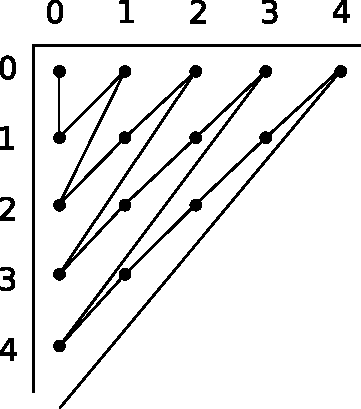
\includegraphics{img/dovetail.pdf}
\end{figure}

Un altro strumento che viene utilizzato \`e la codifica di coppia. Tale strumento viene utilizzato molto spesso in calcolabilit\`a, ed \`e alla base (una volta generalizzato per un numero arbitrario di argomenti) del meccanismo per cui possiamo sempre approssimare una funzione con $N$ argomenti con una funzione ad $n$ argomenti con $N>n$. Praticamente questa ci permette di associare ad ogni possibile coppia un numero naturale e viceversa, in questo modo:

\begin{equation}\left\langle x,y \right\rangle = 2^x(2y+1)-1.\end{equation}

La funzione di codifica \`e reversibile, cio\`e dato il numero che codifica la coppia possiamo calcolare i due numeri che la formano:

\begin{equation}\pi_{1}(z) = \mu x((z+1)/2^x\ sia \ dispari)\end{equation}
\begin{equation}\pi_{2}(z) = ((z+1)/2^{\pi_{1}(z)} -1)/2 \end{equation} 

Questo metodo sar\`a pi\`u utilizzato della coda di rondine, in quanto, oltre a darci un ordine con cui scorrere tutte le coppie, ci permette di associarle ad un numero e di passare in modo molto veloce da numero a coppia e da coppia a numero. Inoltre, la codifica di coppia pu\`o essere utilizzata per codificare triplette o n-uple di numeri. Per le triplette basta, ad esempio, codificare come coppia gli ultimi due elementi, ottenendo cos\`i una coppia, e poi codificare questa di nuovo.

% ALESSANDRO

\section{Predicati e insiemi}

%%%%%%%%%%%%%%%%%%%%%%%%%%%%%%%%%%%%%%%%%%%%%%%
%
% PREDICATI E INSIEMI
%
%%%%%%%%%%%%%%%%%%%%%%%%%%%%%%%%%%%%%%%%%%%%%%%

Data la necessit\`{a} di introdurre il concetto di \textit{predicato}, \`{e} importante notare che:
\begin{itemize}
 \item un predicato si dice \textit{decidibile} quando si \`{e} costruttivamente in grado di determinare se esso vale o non vale su di un argomento
 \item un predicato si dice \textit{semidecidibile} quando si \`{e} costruttivamente in grado di determinare solo se se esso vale su di un argomento, mentre non si \`{e} in grado di farlo per quando non vale
\end{itemize}
Se si considerano le procedure effettive che caratterizzano se un predicato vale (o non vale) su di un argomento, \`{e} facile notare una diretta corrispondeza tra:
\begin{itemize}
 \item la procedura che caratterizza un predicato decidibile e la funzione caratteristica di un insieme ricorsivo
 \item la procedura che caratterizza un predicato semidecidibile e la funzione semicaratteristica di un insieme semidecidibile
\end{itemize}
in quanto gli elementi su cui il predicato vale formano un insieme che \`{e} il dominio della procedura che caratterizza il predicato stesso e, se la procedura è ricorsiva, e ovvio notare come tale insieme \`{e}:
\begin{itemize}
 \item \textit{ricorsivo} se il predicato \`{e} decidibile
 \item \textit{r.e.} se il predicato \`{e} semidecidibile
\end{itemize}
Nei teoremi che seguono quindi (e comunque in generale), i teoremi dimostrati per i predicati semidecidibili verranno assunti come validi anche per gli insiemi r.e..

%%%%%%%%%%%%%%%%%%%%%%%%%%%%%%%%%%
%
% N GODEL
%
%%%%%%%%%%%%%%%%%%%%%%%%%%%%%%%%%%

\section{Numero di G\"odel}

\begin{thm} Teorema di Forma Normale (Kleene [1936]):
Esiste una funzione primitiva ricorsiva $ U(x)$ e per ogni n $\ge1$ un predicato decidibile $T_{n} \left( e,\overrightarrow{x},z \right)$ tali che per ogni funzione ricorsiva $\varphi$ ad $n$ variabili esiste un numero $e$ per cui vale:
\begin{enumerate}
\item $\varphi^{\left( n \right)} \left( \overrightarrow{x}\right)\downarrow$ se e solo se $\exists z T_{n} \left(  e  , \overrightarrow{x}  , z \right)$  ;
\item $\varphi^{\left( n \right)}_{e} =  U \left( \mu  z   T_{n}\left( e,\overrightarrow{x},z\right) \right)   $ ;
\end{enumerate}
\end{thm}

$T_{n} \left( e,\overrightarrow{x},z \right)$ \`e chiamato "`Predicato T di Kleene"' e informalmente si legge: la macchina di Turing (o procedura equivalente per la \textit{Tesi di Church}) con indice $e$, applicata all'input $\overrightarrow{x}$ si ferma in $z_{1}$ passi con output $z_{2}$. L'argomento $z$ \`e la codifica della coppia $\langle  z_{1} , z_{2} \rangle$. Questo predicato \`e decidibile (ovvero la funzione che lo calcola \`e totale) dato che viene posto un limite rigido al numero di passi che la macchina deve eseguire cio\`{e} $z_1$.\\
In altri termini il predicato consiste di una procedura effettiva che esegue $z_1$ passi della e-esima macchina di Turing per poi andare a vedere se la macchina ha terminato, e se lo ha fatto, se ha ritornato il valore $z_1$, quindi sar\`{a} sempre in grado di dare una risposta, su ogni input $\Rightarrow$ \`{e} un predicato decidibile.\\
La codifica di coppia fa s\`i che vengano testati tutti i possibili valori di $z_1$ e $z_2$.\\
$U(x)$ \`{e} la funzione primitiva ricorsiva che prende la seconda componente della codifica di coppia dello $z$ per cui il predicato \textit{T di Kleene} vale.

\paragraph{\textbf{Un esempio molto informale}}

Per usare una metafora molto pittoresca, supponiamo di avere un appuntamento con la nostra ragazza (o ragazzo) al parco e che la funzione ricorsiva da calcolare sia "`la mia ragazza \`e arrivata"'. Se la nostra ragazza arriva puntuale \`e facile rispondere di s\`i immediatamente. Anche se il ritardo \`e breve, ad esempio 5 minuti, decidere se lei \`e arrivata \`e un compito abbastanza facile. Cosa succede per\`o se il ritardo si f\`a pi\`u consistente? L'unico modo per essere assolutamente certi che lei non arriver\`a, \`e di continuare ad aspettarla. Se per esempio dopo 2 settimane decidessimo arbitrariamente che lei non arriver\`a e lasciassimo il parco, lei potrebbe sempre arrivare con un ritardo di 2 settimane e 5 minuti. Per poi sentirci rinfacciare di esserci dimenticati! Allo stesso modo per\`o, continuare ad aspettare ci pone davanti allo spiacevole rischio di invecchiare all'infinito sulla panchina del parco in sua attesa. L'unica soluzione ragionevole \`e di decidere dopo un margine abbastanza largo se la nostra ragazza \`e venuta al nostro appuntamento oppure no.

Il predicato \textit{T di Kleene} \`e equivalente, per le funzioni ricorsive, a ci\`o che farebbe una persona normale in occasione di un appuntamento. Fissa un tempo limite (un determinato numero di passi nel nostro caso) per stabilire se per una determinata funzione ricorsiva con un determinato input si \`e avuta una convergenza su un determinato output.\\


Possiamo quindi considerare il numero $e$ come l'indice della funzione parziale ricorsiva per cui valgono (1) e (2) ed introdurre la nostra specifica notazione:
\begin{defi}
$
\varphi^{n}_{e} \left( o \left\lbrace e  \right\rbrace^n  \right)
$
\`e l' e-esima funzione parziale di n va\-ria\-bi\-li:
\[
\varphi^{\left( n \right)}_{e} \left( \overrightarrow{x}\right)\downarrow\ =\ U \left( \mu  z T_{n}\left(e,x_1,....,x_n,z \right) \right)
\]
\end{defi}
Il seguente teorema \`e una forma simmetrica del \textit{Teorema di Forma Normale di Kleene}:

\begin{thm}
Teorema di Enumumerazione: La sequenza $ \left\lbrace   \varphi^{n}_{e} \right\rbrace_{e \in w} $ \`e un elemento della enumerazione di funzioni parziali, nel senso che:

\begin{enumerate}
\item Per ogni e, $\varphi^{n}_{e}$ \`e una funzione parziale ricorsiva di $n$ variabili
\item Se $\psi$ \`e una funzione parziale ricorsiva di $n$ variabili, allora esiste un e tale che $\psi = \varphi^{n}_{e}$
\end{enumerate}
\end{thm}

\begin{proof}
Tutto segue dal Teorema di Forma Normale e dalla definizione di $\varphi^{n}_{e}$ :
$$\varphi \left( e,\overrightarrow{x} \right) = U \left( \mu  z   T_{n}\left( e,\overrightarrow{x},z\right) \right)$$
\end{proof}

L'indice di una funzione, conosciuto come numero di G\"odel, \`e un concetto molto importante che permette di identificare ogni possibile funzione ricorsiva (e quindi ogni possibile programma o macchina di Turing o procedura equivalente per la \textit{Tesi di Church}) e allo stesso tempo di riassumere ogni programma con un singolo numero. Questo \`e un concetto chiave della teoria della ricorsione, che aggiunge nuovo significato (oltre a quello immediato) ai numeri. Da questo momento in poi infatti, un numero non sar\`a pi\`u soltanto un input, un output o un pezzo di programma, ma un programma stesso. In ogni momento un programma potr\`a quindi fare riferimento ad un altro programma semplicemente "`chiamandolo per nome"' (cio\`e per il suo indice). Si potr\`{a} fornire come input a un programma un altro programma o restituire come output un programma. Cosa pi\`u incredibile, usando il suo indice un programma potr\`a riferirsi a se stesso durante la sua stessa computazione.

%%%%%%%%%%%%%%%%%%%%%%%%%%%%%%%%%%%%%%%%%%%%%%%
%
% PREDICATI
%
%%%%%%%%%%%%%%%%%%%%%%%%%%%%%%%%%%%%%%%%%%%%%%%

\section{Proprietà dei predicati semidecidibili}

\begin{thm}[Teorema di struttura]
$P(x)\subseteq\mathbb{N}^{k}$ predicato decidibile sse esiste $Q(x,z)\subseteq\mathbb{N}^{k+1}$ decidibile t.c. $P(x)=\exists z\ Q(x,z)$.
\end{thm}

\begin{proof}
($\Leftarrow$) sia $P(x)$ semidecidibile.\\
Possiamo quindi scrivere la sua funzione semicaratteristica
$$SC_{P}(x)\ converge\ a\ 1\ sse\ P(x)$$
che per definizione di insieme r.e. \`{e} una funzione ricorsiva.\\
Dato che ogni funzione ricorsiva \`{e} enumerabile esiste un $e\in\mathbb{N}$ per cui
$$SC_{P}(x)=\varphi_{e}(x)$$
Usando ora il predicato \textit{T di Kleene} possiamo scrivere
$$SC_{P}(x)=\exists z\ T(e,x,z)$$
Il predicato \textit{T di Kleene} \`{e} decidibile e, fissato $e$, possiamo scriverlo come $Q(x,z)$
$$SC_{P}(x)=\exists z\ Q(x,z)$$
Intuitivamente il teorema dice che nel cercare uno $z$ tale che $Q$ valga, partendo dal minimo $z$, se non lo si trova, si va avanti all'infinito.\\

($\Rightarrow$) sia $P(x)=\exists\ z Q(z,x)$ con $Q$ predicato decidibile.\\
Per dimostrare che $P(x)$ \`{e} semidecidible scriviamo la sua funzione semicaratteristica
$$SC_{P}(x)=s(z(\mu z.\ 1-\chi_{Q}(x,z)))$$
$SC_{P}$ \`{e} ricorsiva perch\'{e} definita per composizione di funzioni ricorsive ($\chi_{Q}$ \`{e} ricorsiva perch\'{e} $Q$ \`{e} decidibile) e minimalizzazione illimitata.
Quindi $P$ per la definizione di funzione semicaratteristica \`{e} semidecidibile.
\end{proof}
Questo teorema evidenzia come gli insiemi ricorsivi non siano chiusi rispetto all'esistenziale in quanto nel caso di un valore che non appartenga al dominio dell'insieme ricorsivo l'esistenziale divergerebbe.

\begin{thm}[Teorema di proiezione]
Sia $P(x,y) \subseteq\mathbb{N}^{k+1}$ predicato semidecidibile. Allora $S(x) = \exists x\ P(x,y)$ \`{e} semidecidibile.
\end{thm}

\begin{proof}
sia $P(x,y)$ semidecidibile.\\
Allora per il \textit{Teorema di struttura} esiste $Q(t,x,y)$ decidibile tale che:
$$P(x,y) = \exists t\ Q(t,x,y)$$
quindi possiamo riscrivere la conclusione del teorema come
$$S(x) = \exists x\ \exists t\ Q(t,x,y)$$
Usiamo ora la codifica di coppia per scorrere tutte le coppie $\langle x,t \rangle$ con un $w\subseteq\mathbb{N}$:
$$S(x) = \exists w\ Q(\pi_{2}(w),\pi_{1}(w),y)$$
che notiamo essere l'esistenziale di un predicato decidibile.
Per il \textit{Teorema di struttura} possiamo dunque concludere che $S(x)$ \`{e} semidecidibile.
\end{proof}
Anche questo teorema ci fornisce una nozione importante sugli insiemi, cio\`{e} che gli insiemi r.e. sono chiusi rispetto all'esistenziale, a differenza degli insiemi ricorsivi.

%%%%%%%%%%%%%%%%%%%%%%%%%%%%%%%%%%%%%%%%%%%%%%%
%
% CARATTERIZZAZIONI
%
%%%%%%%%%%%%%%%%%%%%%%%%%%%%%%%%%%%%%%%%%%%%%%%

\section{Caratterizzazione insiemi ricorsivi ed r.e. (continua)}

\begin{thm}
 \label{thm:2}
(Post[1943], Kleene[1943], Mostowski [1947]) Un insieme $A$ \`e ricorsivo se e solo se $A$ \`e r.e. e $A$ possiede un complementare $\bar{A}$ r.e..
\end{thm}

\begin{proof}

($\Rightarrow$) Assumendo che $A$ sia ricorsivo, per dimostrare che entrambi $A$ ed $\bar{A}$ sono r.e., definiamo le rispettive funzioni semicaratteristiche e le scriviamo come funzioni ricorsive:\\

$SC_{A}(x)\ converge\ a\ 1\ sse\ C_{A}(x) = 1 \Rightarrow SC_{A}(x) = s(z(\mu w.\ 1 - C_{A}(x)))$\\

$SC_{\bar{A}}(x)\ converge\ a\ 1\ sse\ C_{A}(x) = 0 \Rightarrow SC_{\bar{A}}(x) = s(z(\mu w.\ C_{A}(x)))$\\

Notiamo come l'utilizzo della minimalizzazione illimitata con parametro $w$ applicata ad un argomento inidipendente da $w$ stesso sia l'espediente che abbiamo per far divergere tutta la funzione nel caso non si verifichi proprio il valore che ci aspettiamo di $C_{A}(x)$.\\
Avendo definito due funzioni parziali ricorsive che hanno come dominio rispettivamente $A$ e $\bar{A}$, per la definizione di insieme r.e. possiamo concludere che $A$ e  $\bar{A}$ sono r.e..\\

($\Leftarrow$) Per dimostrare questa implicazione \`{e} necessario tenere presente che $A$ e $\bar{A}$ sono complementari per ipotesi, cio\`{e} che $A\cup\bar{A} = \mathbb{N}$.\\
Dati $A$ e $\bar{A}$ r.e., per le loro funzioni semicaratteristiche abbiamo che:
\begin{center}
$x\in{A}\Leftrightarrow SC_{A}(x)\ converge\ a\ 1$\\\end{center}
\begin{center}
$x\in{\bar{A}}\Leftrightarrow SC_{\bar{A}}(x)\ converge\ a\ 1$\\\end{center}

Ora, per il teorema di struttura dei predicati semidecibili esistono due predicati decidibili $R$ e $Q$ tali che:
\begin{center}
$x\in{A}\Leftrightarrow \exists y R(x,y)$\\\end{center}
\begin{center}
$x\in{\bar{A}}\Leftrightarrow \exists y Q(x,y).$\\\end{center}
con $y$ numero di passi.\\
Dalla premessa che $A\cup\bar{A} = \mathbb{N}$ vale che:\\
\[
\forall x \exists y (R(x,y) \vee Q(x,y))
\]
Definiamo ora la funzione
\[
f(x)=\mu y(R(x,y) \vee Q(x,y))
\]
\`{E} importante notare come solo uno ed esattamente uno tra $R(x,y)$ e $Q(x,y)$ possa valere su di un argomento.\\
$f$ \`{e} ricorsiva totale e ritorna il minimo numero di passi per cui, su un dato argomento $x$, o $R$ o $Q$ vale. Possiamo utilizzare sempre $f(x)$ come numero di passi per i predicati decibili dato che, per quanto visto sopra, solo uno dei due, con $f(x)$ passi varr\`{a}, caratterizzando l'appartennza o meno dell'argomento $x$ all'insieme $A$.\\
Scriviamo quindi la funzione che caratterizza $A$:

$$
c_{A}(x)=\begin{cases}
1\ se\ R(x,f(x))\cr
0\ se\ Q(x,f(x))\end{cases}
$$\\
che essendo una funzione definita per casi, \`{e} ricorsiva.\\
Per la definizione di insieme ricorsivo, concludiamo che $A$ \`{e} ricorsivo.
\end{proof} 

% ANDREA

\section{Un insieme r.e. non ricorsivo}

\begin{thm}
  Esiste un insieme ricorsivamente enumerabile ma non ricorsivo, chiamiamo tale insieme K.
\end{thm}

\begin{proof}
  Vediamo che è possibile definire una funzione di questo tipo:\\

  $\psi(x)=\left\{ \begin{array}{ll}
  1 & se\ \varphi_{x}(x)\ termina\\
  diverge & se\ \varphi_{x}(x)\ diverge\end{array}\right.$\\

  Il nostro scopo è di definire $K$ come dominio di questa funzione $\psi$ e quindi, per dire che $K$ è ricorsivamente
  enumerabile dobbiamo dimostrare che questa funzione è ricorsiva parziale.\\

  Per vedere che $\psi$ è parziale è sufficiente notare che la funzione sempre indefinita è ricorsiva (si può infatti esprimere
  in questo modo: $\mu t . 1$), esiste quindi il suo corrispondente numero di G\"odel $i$ ed è facile vedere che $\psi(i)$ non è definita.
  Quindi $\psi$ è parziale.\\

  $\psi$ è calcolabile (cioè ricorsiva) perchè può essere definita tramite composizione di funzioni ricorsive in questo modo:\\

  $\psi(x) = s(z(\varphi_{x}(x))) = s(z(\mu w\ T_{n}(x,x,w)))$\\

  Infatti se $\varphi_x(x)\downarrow$ (termina), allora esiste una coppia [numero di passi, valore di output] codificata in $w$ che rende
  vero il predicato T di Kleene, ovvero $\exists w\ T_n(x,x,w)\ \grave e\ vero$ e perciò la minimalizzazione termina trovando questo minimo
  valore $w$ e, applicando la funzione zero e successivo, ritorna 1 come voluto.\\
  Se invece $\varphi_x(x)\uparrow$ (diverge), allora non esiste alcun numero di passi per cui $\varphi_x$ termini e in particolare non
  esiste una coppia [numero di passi, valore di output] codificata in $w$ che renda vero il predicato T di Kleene da cui segue che la 
  minimalizzazione non termina e quindi la funzione resta indefinita.\\

  $K$ è quindi un insieme ricorsivamente enumerabile perchè definito come dominio della funzione ricorsiva
  parziale $\psi$. $\psi$ è anche la sua funzione semi caratteristica.\\

  Dimostrato come $K$ sia ricorsivamente enumerabile, dobbiamo dimostrare che non è ricorsivo.\\

  Assumiamo che $K$ sia ricorsivo, allora per il Teorema \ref{thm:1} $\bar{K}$ è ricorsivamente enumerabile, cioè 
  $\exists\ m\ .\ \bar{K} = Dom(\varphi_{m})$.\\
  Da questo segue che $m \in \bar{K} \iff m \in Dom(\varphi_{m})$, ma dalla funzione semicaratteristica di $K$ ($\psi$) segue anche che
  $m \in K \iff m \in Dom(\varphi_{m})$; siamo dunque arrivati alla contraddizione per cui $m$ apparterrebbe sia a $K$ che a $\bar{K}$ e
  questo è dovuto al fatto che abbiamo supposto $K$ essere un insieme ricorsivo.\\

  Dunque $K$ è un insieme ricorsivamente enumerabile e non ricorsivo.
\end{proof}

Notiamo come $K$ corrisponda all'insieme degli indici delle funzioni calcolabili che terminano sul proprio indice.\\
Detto in altre parole, l'indice $i$ di una funzione calcolabile (che altro non è se un numero naturale)
appartiene a $K$ se e solo se la $i$-esima funzione calcolabile termina sull'argomento $i$ stesso.\\

Nel teorema appena dimostrato abbiamo anche incontrato  il primo esempio di insieme non ricorsivamente enumerabile; $\bar{K}$ è infatti
non r.e. perchè se lo fosse seguirebbe, per il Teorema \ref{thm:2}, che $K$ sarebbe ricorsivo.\\

E' importante sottolineare le seguenti cose:
\begin{itemize}
  \item Dato un qualsiasi elemento appartenente a $K$ possiamo effettivamente decidere che tale elemento vi appartiene tramite la sua funzione semicaratteristica.
  \item Dato un qualsiasi elemento non appartenente a $K$ non possiamo decidere che tale elemento non deve appartenervi perchè la sua funzione semicaratteristica
    non ci darebbe mai una risposta (diverge)
  \item Dato un qualsiasi elemento appartenente a $\bar{K}$ non possiamo decidere che tale elemento deve effettivamente appartenere a $K$ perchè non esiste alcuna
    funzione che terminerebbe dandoci risposta affermativa
\end{itemize}

\section{Una caratterizzazione classica non valida intuizionisticamente}

Enunciamo ora un teorema che fornisce un'ulteriore caratterizzazione degli insiemi r.e. che ci viene dalla logica classica.

\begin{thm}
  Un insieme $A$ \`e ricorsivamente enumerabile se e solo se $A$ è l'insieme vuoto oppure $A$ è immagine di una funzione totale ricorsiva
\end{thm}

Questo teorema ci fornisce un'altra definizione di insieme r.e. valida classicamente, che per\`o intuizionisticamente
non possiamo accettarla in quanto non possiamo fornire un metodo costruttivo per stabilire se un insieme $A$ qualunque sia abitato oppure no.\\
Cioè, se ci viene dato $A$ non possiamo sapere se $x \in A$ perch\'e vorrebbe dire
$\exists x \in A\left(x \right) \vee \neg\exists x \in A \left(x \right)$, cio\`e la regola del terzo escluso.
Un calcolatore non saprebbe calcolarlo.\\

Possiamo tuttavia "`correggere"' il teorema precedente limitandolo agli insiemi abitati e rendendolo quindi costruttivo:
\begin{thm}
  Un insieme $A$ abitato è ricorsivamente enumerabile se e solo se $A$ è immagine di una funzione totale ricorsiva
\end{thm}

\begin{proof}

  ($\Leftarrow$) Questo verso della dimostrazione è molto semplice, infatti per dimostrare che $A$ è r.e.
  ci basta definire la sua funzione semicaratteristica ed essendo $A = img(f)$, con $f$ una funzione totale
  ricorsiva, possiamo ottenerla in questo modo:
  
  \[
    SC_A(x) = s(z(\mu y\ f(y) = x))
  \]

  Praticamente cerchiamo il minimo argomento di $f$ che ha $x$ come immagine e abbiamo due casi:
  \begin{itemize}
    \item se $x \in A$ significa che $\exists y\ f(y) = x$, la minimalizzazione termina trovando
      il minimo valore di $y$ e applicando la funzione zero e successivo restituisce 1
    \item se $x \notin A$ significa che $\nexists y\ f(y) = x$, la minimalizzazione quindi non termina
      e $SC_A$ diverge
  \end{itemize}

  E' importante sottolineare che è possibile procedere in questo modo perchè $f$, essendo una funzione totale, è
  sempre definita e ci permette quindi di scorrere tutti i suoi possibili argomenti eseguendola.

  ($\Rightarrow$) 
  Dimostriamo ora il verso contrario; vogliamo cioè scrivere una funzione $f$ totale ricorsiva la cui immagine sia l'insieme $A$.\\
  Dall'ipotesi che $A$ \`e abitato viene $\exists a_0 \in A$. Siccome siamo in ambito
  intuizionistico siamo anche in grado di fornire tale $a_0$. Sappiamo inoltre, per definizione di r.e., che $A = dom\left(\psi \right)$
  con $\psi$ ricorsiva parziale (cioè calcolabile) e quindi esiste un indice $e$ per cui $\varphi_e = \psi$.\\
  Partendo dall'elemento $a_0 \in A$, da questa funzione $\psi$, e in particolare dal suo indice $e$, cerchiamo di costruire la funzione $f$ cercata.\\

  L'idea è quella di definire la funzione $f$ in modo che interpreti il suo argomento $x$ come una coppia codificata secondo la 
  ``codifica di coppia'' illustrata precedentemente e cioè come i due numeri $\pi_1(x)$ e $\pi_2(x)$.\\
  A questo punto $f$ ritonerà $\pi_1(x)$ se $\pi_1(x) \in Dom(\psi)$, cioè se l'esecuzione di $\psi(\pi_1(x))$ termina in un certo
  numero di passi e con un certo valore codificati come coppia dal secondo numero $\pi_2(x)$.\\
  Se così non fosse $f$ restituirà comunque il valore $a_0$ che sappiamo appartenere ad $A$.\\
  Considerando e limitandoci ad un certo numero di passi dell'esecuzione di $\psi$ ci assicuriamo che la funzione risultante sia totale
  come richiesto.\\

  Per definire la nostra funzione sfruttiamo il Predicato di Kleene $T\left(x,y,z \right)$ che è decidibile e che abbiamo introdotto
  nell'enunciazione del Teorema di Forma Normale.\\
  Ricordiamo inoltre che $z$ \`e la codifica della coppia $\left\langle z_1,z_2 \right\rangle$.\\
  Con queste considerazioni costruiamo la funzione $f$ la cui immagine sarà l'insieme $A$:

  $$
    f(x)=\left\{ \begin{array}{cc}
      a_0 & se\ T_n(e,\pi_{1}(x),\pi_{2}(x))\ \grave e\ FALSO \\
      \pi_{1}(x) & se\ T_n(e,\pi_{1}(x),\pi_{2}(x))\ \grave e\ VERO \end{array}\right.
  $$

  Notiamo che:
  \begin{itemize}
    \item la funzione $f$ è totale in quanto il predicato $T_n$ è decidibile e in entrambi i casi (sia che sia vero o falso) viene restituito un valore
    \item i valori che la funzione $f$ ritorna (quindi la sua immagine) sono elementi che appartengono all'insieme $A$, infatti:
    \begin{itemize}
      \item $a_0$ è l'elemento che sappiamo appartenere ad $A$ che è non vuoto
      \item $\pi_1(x) \in Dom(\psi) = A$ perchè se il predicato $T_n(e, \pi_1(x), \pi_2(x))$ è vero significa che $\varphi_e(\pi_1(x))$
        termina e restituisce un certo valore in un certo numero di passi, cioè che $\pi_1(x) \in Dom(\varphi_e)$, ma $e$ è proprio
        l'indice della funzione $\psi$ (cioè $\varphi_e = \psi$) e quindi $\pi_1(x) \in Dom(\psi) = A$
    \end{itemize}
  \end{itemize}

  $\\$Verifichiamo ora formalmente che $img(f) = A$:

  \begin{description}
    \item[$img(f) \subseteq A$]$\\$
      $m \in img(f)$ e abbiamo due casi:
      \begin{itemize}
        \item
          $m = a_0 \implies m \in A$
        \item
          $
            \exists\ w = \pi(m,z)\ .\ T(e, \pi_1(w), \pi_2(w))\ vero \implies \exists\ w = \pi(m,z)\ .\ T(e, m, z)\ vero \\ 
            \implies \varphi_e(m) \downarrow \implies m \in dom(\varphi_e) \implies m \in dom(\psi) \implies m \in A
          $
      \end{itemize}
    \item[$A \subseteq img(f)$]$\\$
      $
        m \in A \implies m \in dom(\psi) \implies m \in dom(\varphi_e) \implies
        \exists\ \langle z_1, z_2 \rangle\ .\ \varphi_e(m)\downarrow in\ z_1 \text{ passi con valore } z_2 \implies
        \exists\ z\ .\ T(e,m,z)\ vero \implies \exists\ w = \pi(m,z)\ .\ f(w) = \pi_1(w) \implies f(w) = m \implies m \in img(f)
      $
  \end{description}

  $\\$Quindi $img(f) = A$.
\end{proof}

\begin{thm}
  Ogni insieme r.e. infinito, contiene un sottoinsieme ricorsivo infinito
\end{thm}

\begin{proof}
  Sia $A$ un insieme r.e. infinito. Per il teorema precedente $A$ è immagine di una funzione totale ricorsiva $f$.\\
  Definiamo $g$ ricorsiva e crescente nel modo seguente:

  $$g(0) = f(0)$$
  $$g(n+1) = f(\mu y(f(y)>g(n))).$$\\
  Dove la seconda riga si legge anche "`$g(n+1)$ \`e uguale al primo elemento generato in $A$ e pi\`u grande di $g(n)$"'\\

  Allora $g$ è una funzione ricorsiva (perchè definita per ricorsione primitiva a partire da funzioni ricorsive), non decrescente,
  per il teorema \ref{thm:3} la sua immagine è un insieme ricorsivo che è anche un sottoinsieme infinito di $A$ per definizione.
\end{proof}

\section{Problema della fermata}

Esiste una procedura effettiva tale che, dati $x$ ed $y$ qualsiasi, è
in grado di determinare se $\varphi_{x}(y)$ termina?

Per la tesi di Church questa domanda pu\`o essere posta, pi\`u precisamente,
nella seguente forma: esiste una funzione ricorsiva $g$ totale tale
che $g(x,y)=1$ se $\varphi_{x}(y)$ è definita e $g(x,y)=0$
se $\varphi_{x}(y)$ diverge?\\

La risposta sta nel seguente teorema:

\begin{thm}
  Non esiste una funzione ricorsiva $g$ tale che, per ogni x, y:\\

  $g(x,y)=\left\{ \begin{array}{ll}
  1 & se\ \varphi_{x}(y)\ termina\\
  0 & se\ \varphi_{x}(y)\ non\ termina\end{array}\right.$
\end{thm}

\begin{proof}
  Assumiamo che esista una tale $g$ ricorsiva.\\
  Sfruttando $g$ possiamo definire la funzione caratteristica dell'insieme $K$:\\

  $
    C_K(x)=\left\{ \begin{array}{ll}
    1 & se\ \varphi_x(x)\ termina\\
    0 & se\ \varphi_x(x)\ non\ termina\end{array}\right.
    =
    \left\{ \begin{array}{ll}
    1 & se\ g(x,x)=1\\
    0 & se\ g(x,x)=0\end{array}\right.
  $\\

  $C_K$ è una funzione totale e se riusciamo a dimostrare che è anche calcolabile, cioè ricorsiva, significa
  che $K$ possiede una funzione caratteristica e che quindi $K$ è ricorsivo.\\

  $C_K$ si può definire banalmente in questo modo: $C_K(x) = g(x,x)$\\

  Quindi $C_K$ è una funzione totale e ricorsiva perchè composizione di una funzione ricorsiva e quindi l'insieme $K$,
  che sappiamo essere non ricorsivo, è ricorsivo.\\
  Questa è una evidente contraddizione nata dal fatto che abbiamo supposto esistere una tale $g$ ricorsiva; quindi una tale
  funzione $g$ non esiste.
\end{proof}

\begin{thm}
  Non c'è nessuna procedura effettiva per decidere, dato un qualsiasi
  $x$, se $\varphi_{x}$ \`e o meno una funzione totale. Ovvero, non
  esiste nessuna funzione ricorsiva tale che:\\

  $f(x)=\left\{ \begin{array}{ll}
  1 & se\ \varphi_{x}\ \grave e\ totale\\
  0 & se\ \varphi_{x}\ non\ \grave e\ totale\end{array}\right.$
\end{thm}

\begin{proof}
  
  Supponiamo che una tale funzione ricorsiva $f$ esista. Possiamo quindi definire la seguente funzione $g$:

  $
    g(x)=\left\{ \begin{array}{ll}
    \varphi_x(x)+1 & se\ \varphi_{x}\ \grave e\ totale\\
    1 & se\ \varphi_{x}\ non\ \grave e\ totale\end{array}\right.
    =
    \left\{ \begin{array}{ll}
    \varphi_x(x)+1 & se\ f(x) = 1\\
    1 & se\ f(x) = 0\end{array}\right.
  $\\

  E' evidente la totalità di $g$, dimostriamo che è anche calcolabile, cioè ricorsiva, definendola in questo
  modo:\\

  $g(x) = \pi_2(\mu z\ (T_n(x,x,z) \vee f(x)=0)) f(x) + 1$\\

  Verifichiamo che quella riportata è una corretta definizione di $g$:\\
  \begin{itemize}
    \item Se $\varphi_x$ è totale, la minimalizzazione cerca il minimo $z$ che rende vero il predicato
      $T_n(x,x,z) \vee f(x)=0$. Essendo $\varphi_x$ totale, $f(x)=1$ quindi la minimalizzazione si fermerà
      al minimo $z$ che rende vero il predicato di Kleene $T_n(x,x,z)$ cioè alla minima coppia 
      $\langle z_1,z_2 \rangle$ per cui $\varphi_x(x)$ termina con output $z_2$ in $z_1$ passi.
      Di questo $z$ codificato come coppia viene presa (tramite la funzione $\pi_2$) la seconda componente,
      cioè il valore di output della funzione, ovvero il valore corrispondente a $\varphi_x(x)$.\\
      Infine viene sommata l'unità ottenendo quindi il valore $\varphi_x(x) + 1$.
    \item Se $\varphi_x$ non è totale, la minimalizzazione cerca il minimo $z$ che rende vero il predicato
      $T_n(x,x,z) \vee f(x)=0$. Essendo $\varphi_x$ non totale, $f(x)=0$ quindi il predicato risulta vero immediatamente
      e la minimalizzazione ritorna quindi il primo valore testato, cioè zero.\\
      Infine a zero viene sommata l'unità ritornando quindi il valore 1.
  \end{itemize}

  In questo modo abbiamo visto che $g$ è ricorsiva perchè definibile per composizione di funzioni ricorsive, in particolare
  perchè abbiamo assunto che la funzione $f$ esista e sia ricorsiva.\\

  E' importante notare come la funzione $g$ appena definita sia totale perchè ora dimostreremo che, per argomento diagonale, 
  $g$ è diversa da tutte le funzioni totali arrivando quindi ad una contraddizione:\\

  Per ogni $x$ tale che $\varphi_x$ è una funzione totale, $g \neq \varphi_x$ quando applicata ad $x$, infatti:

  \[
  g(x) \neq \varphi_x(x)
  \]

  \[
  \varphi_x(x) + 1 \neq \varphi_x(x)
  \]\\
  Quindi $g$, che è una funzione totale, è diversa da ogni funzione totale di indice $x$ sull'argomento $x$. Questa è una contraddizione
  dovuta al fatto che abbiamo supposto esistere la funzione $f$ di partenza. Una tale funzione $f$ quindi non esiste. 
\end{proof}
\chapter{Sistema assiomatico HA}
\section{Introduzione}

Quotidianamente l'uomo al fine di argomentare, strutturare discorsi e giungere a conclusioni fa uso della logica e di un linguaggio formale ben preciso che gli permette di evitare ambiguit\`a e ridondanze durante un colloquio.\\
Di fondamentale importanza sono le \emph{deduzioni formali} in quanto forzano la verit\`a delle nostre argomentazioni perch\`e ci permettono di definire in modo chiaro le premesse da cui partiamo e le varie regole di inferenza che utilizziamo per arrivare alla conclusione.\\
Quello che a noi interessa quindi sono le \emph{prove} che portiamo per mostrare se determinate proposizioni sono vere e perch\`e lo sono.\\
Per questo abbiamo bisogno di una \emph{teoria assiomatica formale}, cio\`e di una teoria formale in cui \`e possibile esprimere enunciati e dedurre le loro conseguenze logiche in modo del tutto formale e meccanico.\\
\vspace{0.3 cm}

Una \emph{teoria assiomatica} $T$ nel linguaggio $\mathcal{L}$ \`e determinata da un calcolo logico $L$ e da un insieme $\Sigma$ (anche infinito) di formule di $\mathcal{L}$ chiamate assiomi di $T$. Si dice che $\varphi$ \`e conseguenza logica di $\Gamma$\footnote{Con $\Gamma$ indichiamo l'insieme di tutte le assunzioni (premesse) di $T$} in $T$ se esiste una deduzione in $L$ con conclusione $\varphi$ e assunzioni contenute in $\Gamma \cup \Sigma$. In particolare, si dice che $\varphi$ \`e un teorema di $T$ se esiste una deduzione di $\varphi$ con assunzioni tutte contenute in $\Sigma$


\vspace{0.4 cm}
Gli elementi fondamentali di una teoria assiomatica dunque sono:
\begin{enumerate}
	\item un \textsl{\textbf{linguaggio formalizzato}} $\mathcal{L}$
\item un insieme di enunciati nel linguaggio che trattiamo come \textsl{\textbf{assiomi}} della teoria
\item un \textsl{\textbf{sistema deduttivo}} per costruire prove, ossia per derivare teoremi da assiomi

\end{enumerate}
Il linguaggio formalizzato $\mathcal{L}$ consiste di:
\begin{itemize}
	\item un \underline{alfabeto} $\alpha$ di simboli che possono essere le variabili, i connettivi e i quantificatori e i simboli relazionali
\item \underline{regole di costruzione sintattica} che permettono di determinare quali stringhe finite di simboli di $\alpha$ costituiscono il vocabolario delle costanti individuali (nomi), delle variabili, dei predicati e delle funzioni
	\item \underline{regole per determinare} quali sequenze di parole in questo vocabolario  ci danno \underline{formule} di $\mathcal{L}$
\end{itemize}
\vspace{0.5 cm}
Mentre per quanto rigurda il sistema deduttivo \`e importante specificare che cosa \`e una prova.\\
Una \textbf{prova} \`e \textit{un vettore \textsl{finito} di formule conforme alle regole del sistema e le cui assunzioni appartengono solo al sistema di assiomi}.\\
Dal momento che le prove sono composte da un numero finito di passaggi logici, allora per ogni prova esister\`a solo un numero finito di assiomi coinvolti. \\
Specifichiamo infine che fornire una prova non significa decidere in anticipo se questa prova esiste o meno. Noi siamo interessati non ad argomentazioni semantiche ma a derivazioni nel sistema formale HA, che \`e l'equivalente \textsl{costruttivo} della teoria assiomatica di Peano, di cui parleremo tra breve.

\vspace{0.5 cm}

\underline{Perch\'e ci serve tutto questo?}\\
\vspace{0.2 cm}

Il primo teorema di incompletezza di G\"odel pone dei limiti alle teorie assiomatiche dell'aritmetica, o meglio alle teorie formali assiomatiche dell'aritmetica, il cui linguaggio di base consiste nella definizione della struttura dei numeri naturali, della somma e della moltiplicazione in $\mathbb{N}$ e in un apparato logico del primo ordine.\newline
Quindi, dati gli assiomi che regolano la struttura di una sequenza di naturali e che caratterizzano somma e prodotto esiste sicuramente almeno una proposizione $\phi$, formulata nel dato linguaggio dell'aritmetica di base, della quale non ᅵ possibile dimostrare, a partire dagli assiomi, nᅵ la sua affermazione, nᅵ la sua negazione.\footnote{Notiamo che comunque l'incompletabilit\`a non compromette l'aritmetica che c'\`e alla base.}\\
Questo fatto \`e proprio ci\`o che viene affermato nel primo teorema di G\"odel: ogni teoria aritmetica di base assiomatizzata rimane incompleta, qualsiasi sforzo si faccia per completarla con altri assiomi.\\
Quindi qualsiasi teoria matematica assiomatizzata con un'aritmetica di base costituita dalle operazioni di somma e moltiplicazione in $\mathbb{N}$ deve essere incompleta e incompletabile (consistente e con alcuni enunciati non dimostrabili).

\section{Assiomi di HA}
Definiamo ora il sistema assiomatico PA e di conseguenza il sistema HA. Infatti l'aritmetica di Heyting HA formalizza la teoria intuizionista dei numeri.\\ Essa ha gli stessi assiomi propri dell'aritmetica classica PA, a cui si aggiunge l'apparato deduttivo della logica intuizionista. \\I teoremi di HA sono quindi necessariamente un sottoinsieme proprio dei teoremi di PA. L'assioma di induzione appartiene sia a PA che ad HA e questo riflette le posizioni della matematica intuizionista sul carattere costruttivo della successione dei numeri naturali. Come sappiamo, per far ci\`o, dobbiamo specificare il \textsl{linguaggio}, gli \textsl{assiomi} e il \textsl{sistema di prova deduttivo}.\\
Definiamo dunque:
\begin{enumerate}
 \item \underline{\texttt{il linguaggio al primo ordine LA}}\footnote{LA sta per \textsl{linguaggio dell'aritmetica}}, il cui vocabolario comprende:
\begin{itemize}
	\item [-] la \textsl{costante} individuale $0$
	\item[-] il predicato di \textsl{uguaglianza} "`$=$"' 
	\item[-] la funzione a un solo argomento \textsl{successore} $s(x)$
	\item[-] le funzioni a due argomenti $x+y$ (\textsl{somma}) e $x*y$ (\textsl{moltiplicazione})	
	\item[-] quantit\`a numerabile di variabili $x, y, z, w\ldots$
	\item[-] connettivi logici e quantificatori
	\item[-] i segni $,$, $($, $)$
\end{itemize}
\vspace{.5cm}
\item L'\underline{\texttt{insieme dei termini $Trm$}} \`e definito in modo induttivo come segue:
\begin{itemize}
\item[-] La costante $0$ \`e un termine;
\item[-] Ogni variabile \`e un termine;
\vspace{0.3 cm}
\item[-] 
	$\prooftree
  t_1\in Trm ,t_2\in Trm,\dots,t_n\in Trm
   \justifies
f_n(t_1,t_2,\dots,t_n) \in Trm
\endprooftree$ 
\end{itemize}
\vspace{.5cm}
\item  L'\underline{\texttt{insieme delle formule $Frm$}} \`e definito in modo induttivo come segue:
\begin{itemize}
\item[-] Ogni \textit{formula atomica} \`e una formula\footnote{una formula atomica \`e del tipo $R_n(t_1,t_2,\dots,t_n)$ in cui $t_1,t_2,\dots, t_n$ sono termini e $R_n$ \`e una relazione in LA ad $n$ argomenti}
\item[-] Date $\alpha,\beta \in Frm$, $\alpha \circ \beta \in Frm$, con $\circ$ un qualsiasi connettivo di LA, cio\`e $Frm$  chiuso per i connettivi sopra elencati.
\item[-] 
	$\prooftree
  \alpha \in Frm \qquad x \in Variabili
   \justifies
\forall x.\alpha \in Frm
\endprooftree$ 
\vspace{0.3 cm}
\item[-] 
$\prooftree
  \alpha \in Frm \qquad x \in Variabili
   \justifies
\exists x.\alpha \in Frm
\endprooftree$ 

\end{itemize}
\vspace{.5cm}
\item \underline{\texttt{gli assiomi}} che si basano sui postulati di Peano e li vedremo in dettaglio tra poco
\vspace{.5cm}
\item \underline{\texttt{il sistema di prova deduttivo}} che \`e una qualche versione standard di logica al primo ordine costruttiva (dunque senza assunzione del principio del terzo escluso) con identit\`e (le differenze tra le varie versioni sono insignificanti)
\end{enumerate}\par\ \par\noindent

I \underline{postulati} di Peano, sui quali si basa la nostra teoria, sono:
\begin{enumerate}
	\item[(P1)] $0$ \`e un numero naturale
	\item[(P2)] Se $x$ \`e un numero naturale, allora esiste un altro numero na-turale, detto \textsl{successore} di $x$, denotato con $s(x)$
	\item[(P3)] $0\neq s(x)$ per qualsiasi numero naturale $x$
	\item[(P4)] Se $s(x)=s(y)$ allora $x=y$
	\item[(P5)] Sia $P$ una certa propriet\`a sui numeri naturali. Se $P$ vale per $0$ e se per ogni numero naturale $x$ che gode della propriet\`a si ha che $s(x)$ gode di $P$, allora $P$ vale per ogni naturale (non \`e altro che il \textsl{principio di induzione})
\end{enumerate}\par\ \par\noindent

Gli \underline{\textbf{assiomi}} di HA dunque sono:
\begin{enumerate}
	\item[(A1)] $\vdash 0\neq s(x)$ (corrisponde a (P3))
	\item[(A2)] $s(x)=s(y)\vdash x=y$ (corrisponde a (P4))
	\item[(A3)] $\vdash x+0=x$
	\item[(A4)] $\vdash x+s(y)=s(x+y)$
	\item[(A5)] $\vdash x*0=0$
	\item[(A6)] $\vdash x*s(y)=x*y+x$
	\item[(A7)] Regola di induzione (corrisponde a (P5)):\newline\newline
	$\prooftree
  \Gamma, \varphi(z) \vdash \varphi(s(z))
   \justifies
 \Gamma, \varphi(0) \vdash \varphi(t)
 \using
 {IR}
\endprooftree$.
\end{enumerate}\par\ \par\
Si noti che:
\begin{itemize}
\item (A1) afferma che $0$ non \`e l'immagine di $s$ e questo permette di escludere modelli in cui, iterando la funzione successore, si possa compiere un loop che ritorni al punto di partenza. Nel modello di Peano questo sta a indicare, ad esempio, che $0$ non \`e il "`successivo"' di nessun numero naturale
\item (A2) afferma che $s$ \`e una funzione iniettiva che permette di escludere i modelli in cui, partendo da $0$ e andando avanti ripetutamente da un elemento al successore, si possa tornare su un elemento gi\`a visitato e rimanere confinati in un ciclo. In altre parole si sta dicendo ad esempio che se $s$ sta ad indicare il "`successivo"' di un numero naturale, allora se $s(x)$ e $s(y)$ coincidono, anche i "`numeri"' di partenza necessariamente coincidono
\item (A3) e (A4) sono gli assiomi che definiscono la somma tra due numeri naturali
\item (A5) e (A6) definscono il prodotto tra due numeri naturali
\item (A7) permette di affermare che l'insieme dei naturali $\mathbb {N}$ \`e il pi\`u piccolo insieme che contenga lo $0$ e che contenga il successore di ogni suo elemento (cio\`e che sia chiuso per la funzione s) e quindi permette di escludere modelli in cui siano presenti degli elementi "`intrusi"' al di fuori della sequenza infinita dei successori dello zero
\end{itemize}

\par\ \par\noindent
\underline{\texttt{Osservazione}} Non sono stati dati, almeno esplicitamente, assiomi corrispondenti ai postulati (P1) e (P2). In realt\`a, essi seguono dal fatto che consideriamo $\mathbb{N}$ come dominio di interpretazione e dall'aver definito nel nostro linguaggio la costante $0$ ($0$ \`e automaticamente elemento di $\mathbb{N}$) e la funzione a un solo argomento successore (che vogliamo sia totale, dunque se $x$ \`e un elemento, anche $s(x)$ lo \`e).
\par\ \par\noindent

Questa serie di assiomi sembra per noi sovrabbondante. Infatti, avendo gi\`a l'idea di $\mathbb{N},$ si sarebbe portati a definire i naturali nel modo seguente:\\ 
\emph{definisco $0$ e poi definisco $1$ come il successore di $0$, $2$ come il successore del successore di $0$ e cos\`i via.}\\ 
E' chiaro quindi che i naturali si possono concepire, a partire da $0,$ come una "`linea retta"' di cui consideriamo solo i punti interi positivi.\\
Ma per un robot invece, tali assiomi sono fondamentali per la definizione dei numeri naturali, in quanto non ha modo di costruire la stessa struttura di $\mathbb{N}$ come noi abbiamo in mente.\\
%Questo per\`o un robot (ad esempio) non lo pu\`o fare, in quanto non ha la minima idea della struttura di $\mathbb{N}$ che noi abbiamo in mente.\\ 
Vediamo infatti che cosa succede se forniamo al robot soltanto i postulati P1 e P2: potrebbe costruire i naturali come una "`corona del rosario"' senza cadere in contraddizione con gli stessi. Infatti potrebbe partire dallo $0$, fare ad esempio dieci applicazioni del successore di $0$ e poi chiu-dere il cerchio sullo $0$ iniziale e questo, il robot, lo considererebbe un modello corretto per i naturali, in quanto \`e palese che soddisfa ai due assiomi proposti. \\ L'uomo potrebbe cercare di correggere il tutto inserendo il postulato P3 per far si che $0$ non sia il successore di nessun numero naturale, come vuole la nostra intuizione. Nuovamente, senza cadere in contraddizione, il robot potrebbe costruire un suo modello di $\mathbb{N}$ che neanche lontanamente assomiglia a quello reale, ma che d'altra parte non \`e in contraddizione con P1, P2 e P3 e potrebbe essere una "`corona del rosario"', come nel caso precedente, a cui viene aggiunto (e ovviamente collegato) un "`punto esterno"' (lo zero appunto).\\ Qui non si cade in contraddizione con P3 perch\`e $0$, che \`e esterno alla "`corona"', non ha effettivamente numeri naturali prima di s\`e, d'altra parte i numeri naturali che abbiamo in mente hanno una struttura assai differente. \\ Come si nota, i soli P1, P2 e P3 possono dar luogo a una "`circolarit\`a"', un loop, nella struttura e per eliminare questa possibilit\`a \`e necessario assumere almeno un altro postulato come P4. Si potrebbe pensare che basti quest'ultimo per concludere. Eppure un'ulteriore struttura ben pi\`u complessa renderebbe veri i primi postulati, ma non creerebbe affatto l'idea di $\mathbb{N}$ che vogliamo, n\`e tantomeno la possibilit\`a di indurre su ogni naturale. \\ Ecco perch\`e \`e necessario introdurre anche il postulato di induzione.\\
Bisogna dunque dare al robot l'istruzione: $$\varphi(0) \& \forall z (\varphi(z)\longrightarrow \varphi(s(z))) \vdash \forall z \varphi(z)$$ con $\varphi$ formula.\\
Ma proprio il fornire questa istruzione al robot diventa difficile al programmatore, in quanto bisogna saper scrivere $\varphi$ nel nostro sistema.\\
E' importante sapere che noi, di fatto, stiamo "`sperando"' che quanto fornito sia sufficiente al robot affinch\`e "`capisca"' la nostra intuizione di $\mathbb{N}.$\\ 

\vspace{0.5 cm}
Essendo PA una teoria con uguaglianza, si hanno anche gli assiomi:
\begin{enumerate}
	\item[(U1)] $x=y,x=z\vdash y=z$
	\item[(U2)] $x=y\vdash s(x)=s(y). $
\end{enumerate}
\par\ \par

Potrebbe sembrare che il linguaggio di HA sia povero di espressivit\`a e non ci permetta di parlare di una stringa finita di numeri ma, una volta che abbiamo l'esponenziazione, possiamo semplicemente \textsl{codificare} una sequenza finita di numeri.\\ G\"odel ha mostrato che l'esponenziazione \`e definibile tramite l'introduzione di qualche altra funzione nella nostra aritmetica (la $\beta$-function di cui si parler\`a in seguito). In realt\`a \`e stato provato che essa pu\`o essere introdotta in HA e questo ci permette dunque di codificare sequenze.\\ Quindi potrebbe sembrare che HA dotato di esponenziazione sia pi\`u forte di HA, ma a dire il vero, per quanto appena accennato, sono equivalenti e dunque possiamo eliminare l'esponenziazione dalle nostre assunzioni.\\ Oltre alla potenza di questo linguaggio, verr\`a mostrata pi\`u avanti la consistenza di HA (secondo teorema di G\"odel).  Noi dunque considereremo il sistema assiomatico HA senza estenderlo. \newline
Vedremo come sar\`a possibile definire i concetti di \textsl{numero primo} (che insieme all'esponenziazione \`e comodissimo per codificare, in particolare, sequenze finite di numeri naturali), \textsl{resto della divisione}, \textsl{sottrazione adeguata}, \textsl{divisibilit\`a}, \textsl{relazione d'ordine} e cos\`i via, giusto rimanendo nell'ambito di questa teoria formale. Quindi vedremo come in questo sistema assiomatico sia possibile \textsl{derivare} tutto ci\`o che ci serve per fare matematica. \newline
Si utilizzer\`a il sistema di regole che si basa sul calcolo dei sequenti.

\vspace{0.3 cm}
\subsection{Regole del calcolo dei sequenti}
Il nome "`sequente"' \`e la traduzione dal tedesco della parola {\itshape Sequenz}, introdotta da Gerhard Gentzen nel 1934, ed indica un formalismo che si presenta nella forma:
$$\Gamma_1,\Gamma_2,\dots,\Gamma_m\vdash\Delta_1,\Delta_2,\dots,\Delta_n$$
Il simbolo $\vdash$\ indica che le formule a sinistra (gli {\itshape antecedenti}) sono le ipotesi dalla cui asserzione segue la dichiarazione delle formule a destra (i {\itshape conseguenti}).\\
Occorrono anche altre abbreviazioni come ad esempio:
$$\frac{\Gamma\vdash\Delta}{\Gamma'\vdash\Delta'}$$
dove la barra orizzontale ᅵ dunque un modo veloce per scrivere `"'ci\`o che sta sopra comporta ci\`o che sta sotto"'.\\
Ovvero quello che sta sopra la barra orizzontale deve essere assunto come premessa, mentre quello che sta sotto corrisponde alle deduzioni fatte a partire da tali premesse.\\
Quindi elenchiamo le regole del calcolo dei sequenti (nella versione intuizionista) che utilizzeremo per costruire le prove:
\begin{enumerate}
\vspace{.3cm}
\item[] \textit{Assioma}:
$$\Gamma,A\vdash A \ ax$$

\item[] \textit{Ordine o Scambio}:
$$\prooftree
  A,B \vdash \Delta
   \justifies
 B,A\vdash \Delta
 \using
 {ord}
\endprooftree$$\\
\item[] \textit{Indebolimento}:
$$\prooftree
  \Gamma \vdash \Delta
   \justifies
 \Gamma, \Sigma \vdash \Delta
 \using
 {ind}
\endprooftree$$\\

\item[] \textit{Contrazione}:
$$\prooftree
  \Gamma, A, A \vdash \Delta
   \justifies
 \Gamma, A \vdash \Delta
 \using
 {cont}
\endprooftree$$\\

\item[] \textit{Taglio}:
$$\prooftree
  \Gamma \vdash A\qquad\Gamma', A\vdash \Delta
   \justifies
 \Gamma, \Gamma' \vdash \Delta
 \using
 {cut}
\endprooftree$$\\

	\item[] \textit{Regole per}\ \&:\par\ \par\noindent
$$\prooftree
  \Gamma, A,B \vdash \Delta
   \justifies
 \Gamma, A\ \mbox{\&}\ B \vdash \Delta
 \using
 {\mbox{\&}_{left}}
\endprooftree$$
\hspace{\stretch{1}}

$$\prooftree
  \Gamma \vdash A\qquad\Gamma \vdash B
   \justifies
 \Gamma \vdash A\mbox{\&}B
 \using
 {\mbox{\&}_{right}}
\endprooftree$$\\

\item[] \textit{Regole per $\vee$}:\\
$$\prooftree
  \Gamma, A \vdash \Delta\qquad\Gamma, B \vdash \Delta
   \justifies
 \Gamma, A\vee B \vdash \Delta
 \using
 {\vee_{left}}
\endprooftree$$\\
	$\prooftree
  \Gamma \vdash A
   \justifies
 \Gamma \vdash A\vee B
 \using
 {\vee_{right}}
\endprooftree$
\hspace{\stretch{1}}
$\prooftree
  \Gamma \vdash B
   \justifies
 \Gamma \vdash A\vee B
 \using
 {\vee_{right}}
\endprooftree$
\vspace{.8cm}

\item[] \textit{Regole per $\to$}:\\
$$\prooftree
  \Gamma_1 \vdash A\qquad\Gamma_2, B \vdash \Delta
   \justifies
 \Gamma_1, \Gamma_2, A\to B \vdash \Delta
 \using
 {\to_{left}}
\endprooftree$$\\
$$\prooftree
  \Gamma, A \vdash B
   \justifies
 \Gamma \vdash A\to B
 \using
 {\to_{right}}
\endprooftree$$\\

\item[] \textit{Regole per $\neg$}:\\
$$\prooftree
  \Gamma \vdash A
   \justifies
 \Gamma, \neg A \vdash \Delta
 \using
 {\neg_{left}}
\endprooftree$$\\
$$\prooftree
  \Gamma, A \vdash \bot
   \justifies
 \Gamma \vdash \neg A
 \using
 {\neg_{right}}
\endprooftree$$\\

\item[] \textit{Regole per $\forall$}:\\
$$\prooftree
  \Gamma, A(c) \vdash \Delta
   \justifies
 \Gamma, \forall\ x\ A(x) \vdash \Delta
 \using
 {\forall_{left}}
\endprooftree$$\\
$$\prooftree
  \Gamma \vdash A(z)
   \justifies
 \Gamma \vdash \forall\ x\ A(x)
 \using
 {\forall_{right}\ \mbox{*}}
\endprooftree$$\\

\item[] \textit{Regole per $\exists$}:\\
$$\prooftree
  \Gamma, A(z) \vdash \Delta
   \justifies
 \Gamma, \exists\ x\ A(x) \vdash \Delta
 \using
 {\exists_{left}\ \mbox{*}}
\endprooftree$$\\
$$\prooftree
  \Gamma \vdash A(c)
   \justifies
 \Gamma \vdash \exists\ x\ A(x)
 \using
 {\exists_{right}}
\endprooftree$$

\end{enumerate}
\par\ \par\noindent
\vspace{.3cm}

Contrassegnamo con * le regole in cui $z$ non \`e una variabile libera nel contesto $\Gamma, \Delta$.\\

\section{Espressivit\`a di HA}
Vediamo ora cosa \`e possibile derivare nel nostro sistema assiomatico.\\
Si cercher\`a di dimostrare ogni proposizione tramite una prova, ma si ricorda che le derivazioni non sono uniche e quindi potrebbero esistere altri modi per provare un determinato enunciato.\\
Inoltre prima di cominciare si noti che, per dire che qualcosa \`e derivabile nella nostra teoria, si user\`a il simbolo $\vdash$ anzich\`e $\vdash_{HA}$, ossia si lascia sottinteso il sistema in cui si lavora, salvo specifiche particolari.\\
Valendo: $$\prooftree
\vdash\Gamma\quad\[\vdash\varphi(0)\quad\[\varphi(z),\Gamma\vdash\varphi(s(z))\justifies \varphi(0),\Gamma\vdash \varphi(t)\using{IR}\]\justifies \Gamma\vdash\varphi(t)\using{cut}\]\justifies \vdash\varphi(t)\using{cut}
\endprooftree$$
dimostreremo per tutte le propriet\`a ricorsive solamente $\varphi(0)$ e $\varphi(z)\vdash\varphi(s(z))$. \newline
Infatti, per la validit\`a di:
$$\prooftree
   \vdash \varphi(t)
   \justifies
  \vdash \forall\ x\ \varphi(x)
 \using
 {\forall_{right}}
\endprooftree$$\\
una volta derivati il passo base e il passo induttivo, abbiamo tutti gli strumenti per provare che la propriet\`a $\varphi$ vale per qualunque numero naturale.
\newline
\begin{prop}
Dati $p$, $r$, $t$ termini, in HA valgono le seguenti propriet\`a:
\begin{enumerate}
	\item[(R1)] Simmetria destra:\\ $$\prooftree
  \Gamma \vdash t=r
   \justifies
 \Gamma \vdash r=t
 \using
 {sim_{dx}}
\endprooftree$$
  \item[(R2)] Simmetria sinistra:\\ $$\prooftree
  \Gamma,t=r \vdash\Gamma'
   \justifies
  \Gamma,r=t\vdash\Gamma'
 \using
 {sim_{sx}}
\endprooftree$$
	\item[(R3)] Transitivit\`a:\\ $$\prooftree
  \Gamma \vdash p=t \qquad \Gamma'\vdash t=r
   \justifies
 \Gamma, \Gamma' \vdash p=r
 \using
 {tran}
\endprooftree$$
\end{enumerate}
\end{prop}
\textsc{Dimostrazione} Assumiamo di aver dimostrato (1.2) e (1.3)
\begin{enumerate}
\item[(R1)]
{\scriptsize{
	$$\prooftree
  \Gamma \vdash t=r \qquad t=r\vdash_{1.2} r=t
   \justifies
 \Gamma \vdash r=t
 \using
 {cut}
\endprooftree$$}}
  \item[(R2)]
{\scriptsize{$$\prooftree
	t=r\vdash_{1.2} r=t\qquad \Gamma,r=t\vdash\Gamma'
  \justifies
 \Gamma,t=r \vdash\Gamma'
 \using
 {cut}
\endprooftree$$}}
\item[(R3)]
{\scriptsize{$$\prooftree
  \Gamma' \vdash t=r \qquad  \[\Gamma\vdash p=t\qquad p=t,t=r\vdash_{1.3} p=r\justifies \Gamma, t=r\vdash_{1.3} p=r\using {cut}\]
   \justifies
 \Gamma, \Gamma' \vdash p=r
 \using
 {cut}
\endprooftree$$}}
\end{enumerate}
\hspace{\stretch{1}} $\Box$\\
Usando la propriet\`a simmetria destra si dimostrano:
\begin{enumerate}
	\item[(S1)] $\vdash s(r+p)=r+s(p)$
	\vspace{.2cm}
	\item[(S2)] $\vdash r=r+0$
	\vspace{.2cm}
	\item[(S3)] $\vdash 0+t=t$
	\vspace{.2cm}
	\item[(S4)] $\vdash s(t)\neq 0$
\end{enumerate}
\vspace{.5cm}
\begin{prop}
Per ogni termine $p,\ r,\ t$ valgono:
\begin{enumerate}
	\item[(1.1)] $\vdash t=t$        (riflessivit\`a)
	\vspace{.2cm}
	\item[(1.2)] $t=r\vdash r=t$     (simmetria)
	\vspace{.2cm}
	\item[(1.3)] $p=t,t=r\vdash p=r$ (transitivit\`a)
	\vspace{.2cm}
	\item[(1.4)] $r=t,p=t\vdash r=p$
	\vspace{.2cm}
	\item[(1.5)] $t=r\vdash t+p=r+p$
	\vspace{.2cm}
	\item[(1.6)] $\vdash t=0+t$
	\vspace{.2cm}
	\item[(1.7)] $\vdash s(t)+p=s(t+p)$
	\vspace{.2cm}
	\item[(1.8)] $\vdash t+r=r+t$         (commutativa)
	\vspace{.2cm}
	\item[(1.9)] $t=r\vdash p+t=p+r$
	\vspace{.2cm}
	\item[(1.10)] $\vdash (t+r)+p=t+(r+p)$ (associativa)
	\vspace{.2cm}
	\item[(1.11)] $t=r\vdash t*p=r*p$
	\vspace{.2cm}
	\item[(1.12)] $\vdash 0*t=0$
	\vspace{.2cm}
	\item[(1.13)] $\vdash s(t)*r=t*r+r$
	\vspace{.2cm}
	\item[(1.14)] $\vdash t*r=r*t$         (commutativa)
	\vspace{.2cm}
	\item[(1.15)] $t=r\vdash p*t=p*r$
	\vspace{.2cm}
	\item[(1.16)] $\vdash (t*r)*p=t*(r*p)$ (associativa)
	\vspace{.2cm}
	\item[(1.17)] $p_1=t_1,p_2=t_2,p_1=p_2\vdash t_1=t_2$
	\vspace{.2cm}
	\item[(1.18)] $p_1=t_1,p_2=t_2\vdash p_1+p_2=t_1+t_2$
\end{enumerate}
\end{prop}
\vspace{1cm}
\textsc{Dimostrazione}
\vspace{.2cm}
\begin{enumerate}
\item[(1.1)] [\ $\vdash t=t$\ ]:
\par
{\scriptsize{
	$$\prooftree
	\vdash_{A3} t+0=t\qquad\[\vdash_{A3} t+0=t\qquad t+0=t,t+0=t\vdash_{U1} t=t\justifies t+0=t\vdash t=t\using{cut}\]\justifies \vdash t=t\using{cut}
	\endprooftree$$}}
\\
\item[(1.2)][\ $t=r\vdash r=t$\ ]:
\par
{\scriptsize{$$\prooftree
	\vdash_{1.1} t=t\qquad t=r,t=t\vdash_{U1} r=t \justifies t=r\vdash r=t\using{cut}
	\endprooftree$$}}
%\%justifies t=t,t=r\vdash r=t\using(ord)\
\\
\item[(1.3)][\ $p=t,t=r\vdash p=r$\ ]:
\par
{\scriptsize{	$$\prooftree
	p=t\vdash_{1.2} t=p\qquad t=p,t=r\vdash_{U1} p=r\justifies p=t,t=r\vdash p=r\using{cut}
	\endprooftree$$}}
\\
	\item[(1.4)][\ $r=t,p=t\vdash r=p$\ ]:
\par
{\scriptsize{	$$\prooftree
	p=t\vdash_{1.2} t=p\qquad r=t,t=p\vdash_{1.3} r=p\justifies r=t,p=t\vdash r=p\using{cut}
	\endprooftree$$}}
\\
\item[(1.5)][\ $t=r\vdash t+p=r+p$\ ]:
\vspace{0.5cm}
\\Per induzione su $p$.
\vspace{0.3cm}
\\In questo caso abbiamo: {\scriptsize{$$\varphi(p) :=\ t+p=r+p.$$}}
\\
Passo base:
\par
{\scriptsize{$$\prooftree
	\[\vdash_{A3} t+0=t\qquad t=r\vdash_{ax} t=r\justifies t=r\vdash t+0=r\using{tran}\]\qquad \vdash_{S2}r=r+0\justifies t=r\vdash t+0=r+0\using{tran}
	\endprooftree$$}}
\\
Passo induttivo:
\par
{\scriptsize{$$\prooftree
	\vdash_{A4} t+s(p)=s(t+p)\qquad\[t=r,t+p=r+p\vdash_{U2}s(t+p)=s(r+p)\qquad \vdash_{S1} s(r+p)=r+s(p)\justifies t=r,t+p=r+p\vdash s(t+p)= r+s(p)\using{tran}\]\justifies t=r,t+p=r+p\vdash t+s(p)=r+s(p)\using{tran}
	\endprooftree$$}}
\\
\item[(1.6)][\ $\vdash t=0+t$\ ]:
\vspace{0.5cm}
\\Per induzione su $t$:
\vspace{0.3cm}
\\Passo base: {\scriptsize{$$\vdash_{S2} 0=0+0$$}}
\\Passo induttivo:
\par
{\scriptsize{$$\prooftree
	t=0+t\vdash_{U2} s(t)=s(0+t)\qquad\vdash_{S1} s(0+t)=0+s(t)\justifies t=0+t \vdash s(t)=0+s(t)\using{tran}
	\endprooftree$$}}
\\
\item[(1.7)][\ $\vdash s(t)+p=s(t+p)$\ ]:
\vspace{0.5cm}
\\Per induzione su $p$:
\vspace{0.3cm}
\\Passo base:
\par
{\scriptsize{$$\prooftree
	\vdash_{A3} s(t)+0=s(t)\qquad\[\vdash_{S2}t=t+0\qquad t=t+0\vdash_{U2} s(t)=s(t+0)\justifies \vdash s(t)=s(t+0)\using{cut}\]\justifies \vdash s(t)+0=s(t+0)\using{tran}
	\endprooftree$$}}
	\vspace{0.5cm}
\\Passo induttivo:
\vspace{0.3cm}
\\Dimostriamo prima (1A):
\par
{\scriptsize{$$\prooftree
	\[\vdash_{A4} t+s(p)=s(t+p)\qquad t+s(p)=s(t+p)\vdash_{U2} s(t+s(p))=s(s(t+p))\justifies\vdash s(t+s(p))=s(s(t+p))\using{cut}\]\justifies \vdash s(s(t+p))=s(t+s(p))\using{sim_{dx}}
	\endprooftree$$}}
\vspace{2cm}
quindi si ha:
\par
{\tiny{$$\prooftree
	\vdash_{A4} s(t)+s(p)=s(s(t)+p)\qquad\[s(t)+p=s(t+p)\vdash_{U2}s(s(t)+p)=s(s(t+p))\qquad \vdash_{1A} s(s(t+p))=s(t+s(p))\justifies s(t)+p=s(t+p)\vdash s(s(t)+p)=s(t+s(p))\using{tran}\]\justifies s(t)+p=s(t+p)\vdash s(t)+s(p)=s(t+s(p))\using{tran}
	\endprooftree$$}}
\\
\item[(1.8)][\ $\vdash t+r=r+t$\ ]:
\vspace{0.5cm}
\\Per induzione su $r$.
\vspace{0.3cm}
\\Passo base:
\vspace{0.3cm}
{\scriptsize{$$\prooftree
	\vdash_{A3} t+0=t\qquad \vdash_{1.6} t=0+t\justifies \vdash t+0=0+t\using{tran}
	\endprooftree$$}}
\vspace{0.5cm}
\\Passo induttivo:
\vspace{0.3cm}
{\scriptsize{$$\prooftree \vdash_{A4}t+s(r)=s(t+r)\qquad\[\[\vdash_{1.7}s(r)+t=s(r+t)\qquad\[t+r=r+t\vdash_{U2}s(t+r)=s(r+t)\justifies t+r=r+t\vdash s(r+t)=s(t+r)\using{sim_{dx}}\]\justifies t+r=r+t\vdash s(r)+t=s(t+r)\using{tran}\]\justifies t+r=r+t\vdash s(t+r)=s(r)+t\using{sim_{dx}}\]\justifies t+r=r+t\vdash t+s(r)=s(r)+t\using{tran}
	\endprooftree$$}}
\\
\item[(1.9)][\ $t=r\vdash p+t=p+r$\ ]:
\vspace{0.5cm}
\\Per induzione su $p$.
\vspace{0.3cm}
\\Passo base:
\par
{\scriptsize{	$$\prooftree
	\vdash_{S3} 0+t=t\qquad\[\[\vdash_{S3} 0+r=r\qquad t=r\vdash_{1.2}r=t\justifies t=r\vdash 0+r=t\using{tran}\]\justifies t=r\vdash t=0+r\using{sim_{dx}}\]\justifies t=r\vdash 0+t=0+r\using{tran}
	\endprooftree$$}}
	\vspace{3cm}
\\Passo induttivo:
\vspace{0.3cm}
{\scriptsize{$$\prooftree
	\vdash_{1.7}s(p)+t=s(p+t)\qquad\[t=r,p+t=p+r\vdash_{U2}s(p+t)=s(p+r) \qquad\[\vdash_{1.7} s(p)+r=s(p+r)\justifies \vdash s(p+r)=s(p)+r\using{sim_{dx}}\]\justifies t=r,p+t=p+r\vdash s(p+t)=s(p)+r\using{tran}\]\justifies t=r,p+t=p+r\vdash s(p)+t=s(p)+r\using{tran}
	\endprooftree$$}}
\\
\item[(1.10)][\ $\vdash (t+r)+p=t+(r+p)$\ ]:
\vspace{0.5cm}
\\Per induzione su $p$.
\vspace{0.3cm}
\\Passo base:
\par
{\scriptsize{$$\prooftree
	\vdash_{A3} (t+r)+0=t+r\qquad \[\vdash_{S2} r=r+0\qquad r=r+0\vdash_{1.9}t+r=t+(r+0)\justifies \vdash t+r=t+(r+0)\using{cut}\]\justifies\vdash (t+r)+0=t+(r+0)\using{tran}
	\endprooftree$$}}
\vspace{0.5cm}
\\Passo induttivo:
\vspace{0.3cm}
\\Dimostriamo prima (1B)
\vspace{0.3cm}
  {\scriptsize{$$\prooftree
  \vdash_{A4} (t+r)+s(p)=s((t+r)+p)\qquad (t+r)+p=t+(r+p)\vdash_{U2} s((t+r)+p)=s(t+(r+p))\justifies (t+r)+p=t+(r+p)\vdash (t+r)+s(p)=s(t+(r+p))\using{tran}
	\endprooftree$$}}
	\vspace{0.5cm}
\\e (1C):
\vspace{0.2cm}
  {\tiny{$$\prooftree
  \vdash_{S1} s(t+(r+p))=t+s(r+p)\qquad\[\vdash_{S1} s(r+p)=r+s(p)\qquad s(r+p)=r+s(p)\vdash_{1.9} t+s(r+p)=t+(r+s(p))\justifies \vdash t+s(r+p)=t+(r+s(p))\using{cut}\]\justifies \vdash s(t+(r+p))=t+(r+s(p))\using{tran}
	\endprooftree$$}}
	\vspace{0.5cm}
\\quindi otteniamo:
\vspace{0.3cm}
{\scriptsize{	$$\prooftree
	(t+r)+p=t+(r+p)\vdash_{1B} (t+r)+s(p)=s(t+(r+p))\qquad\vdash_{1C} s(t+(r+p))=t+(r+s(p))\justifies (t+r)+p=t+(r+p)\vdash (t+r)+s(p)=t+(r+s(p))\using{tran}
	\endprooftree$$}}
\vspace{.3cm}
\item[(1.11)] [\ $t=r\vdash t*p=r*p$\ ]:
\vspace{.2cm}
\\Per induzione su $p$, analogamente a (1.5).
\item[(1.12)] [\ $\vdash 0*t=0$\ ]:
\vspace{.2cm}
\\Per induzione su $t$, analogamente a (1.6).
\vspace{0.5cm}
\item[(1.13)] [\ $\vdash s(t)*r=t*r+r$\ ]:
\vspace{.2cm}
\\Per induzione su $r$, analogamente a (1.7).
\vspace{0.5cm}
\item[(1.14)] [\ $\vdash t*r=r*t$ \ ]:
\vspace{.2cm}
\\Per induzione su $r$, analogamente a (1.8).
\vspace{0.5cm}
\item[(1.15)] [\ $t=r\vdash p*t=p*r$\ ]:
\vspace{.2cm}
\\Per induzione su $p$, analogamente a (1.9).
\vspace{0.5cm}
\item[(1.16)] [\ $\vdash (t*r)*p=t*(r*p)$\ ]:
\vspace{.2cm}
\\Per induzione su $p$, analogamente a (1.10).
\vspace{0.5cm}
\item[(1.17)] [\ $p_1=t_1,p_2=t_2,p_1=p_2\vdash t_1=t_2$\ ]:
\vspace{.2cm}
\\Si dimostra usando (1.3), (1.4) e (U1).
\vspace{0.5cm}
\item[(1.18)] [\ $p_1=t_1,p_2=t_2\vdash p_1+p_2=t_1+t_2$\ ]:
\vspace{.2cm}
\\Come il punto precedente\end{enumerate}
\hspace{\stretch{1}} $\Box$\\


\vspace{2cm}
\begin{prop}
Per ogni termine $p,\ r,\ t,$ valgono:
\begin{enumerate}
	\item[(2.1)] $\vdash t*(r+p)=(t*r)+(t*p)$ (distributiva)
	\vspace{.2cm}
	\item[(2.2)] $\vdash (r+p)*t=(r*t)+(p*t)$ (distributiva)
	\vspace{.2cm}
	\item[(2.3)] $t+p=r+p\vdash t=r$ (cancellativa)
\end{enumerate}
\end{prop}
\vspace{.5cm}
\textsc{Dimostrazione}
\vspace{.2cm}
\begin{enumerate}
\item[(2.1)] [\ $\vdash t*(r+p)=(t*r)+(t*p)$\ ]:
\vspace{.5cm}
\\Per induzione su $p$.
\vspace{1cm}
\\Passo base:
\vspace{.2cm}
\\Dimostriamo prima (2A)
\vspace{.2cm}
	{\scriptsize{$$\prooftree
	\[\[\vdash_{A5}t*0=0\qquad t*0=0\vdash_{1.9}t*r+t*0=t*r+0\justifies\vdash (t*r)+(t*0)=t*r+0\using{cut}\]\qquad\vdash_{A3}t*r+0=t*r\justifies\vdash (t*r)+(t*0)=t*r\using{tran}\]\justifies\vdash t*r=(t*r)+(t*0)\using{sim_{dx}}
	\endprooftree$$}}\\
da cui segue
\vspace{.2cm}
	{\scriptsize{$$\prooftree
	\[\vdash_{A3}r+0=r\qquad r+0=r\vdash_{1.15}t*(r+0)=t*r\justifies\vdash t*(r+0)=t*r\using{cut}\]\quad\vdash_{2A} t*r=(t*r)+(t*0)\justifies\vdash t*(r+0)=(t*r)+(t*0)\using{tran}
	\endprooftree.$$}}
	\vspace{.5cm}
\\Passo induttivo:
\vspace{.2cm}
\\Ci serviranno inoltre:
\vspace{.2cm}
\\(2B)
{\scriptsize{	$$\prooftree
	\[\vdash_{A6}(t*s(p))=(t*p)+t\qquad (t*s(p))=(t*p)+t\vdash_{1.9}(t*r)+(t*s(p))=(t*r)+(t*p)+t\justifies\vdash  (t*r)+(t*s(p))=(t*r)+(t*p)+t\using{cut}\]
	\justifies \vdash(t*r)+(t*p)+t=(t*r)+(t*s(p))\using{sim_{dx}}
	\endprooftree$$	}}
	\vspace{.2cm}
	\\(2C)
	{\tiny{$$\prooftree
	t*(r+p)=(t*r)+(t*p)\vdash_{1.5} t*(r+p)+t=(t*r)+(t*p)+t\qquad
	\vdash_{2B}(t*r)+(t*p)+t=(t*r)+(t*s(p))\using{tran}
	\justifies t*(r+p)=(t*r)+(t*p)\vdash t*(r+p)+t=(t*r)+(t*s(p))
	\endprooftree$$	}}
	\vspace{.2cm}
	\\(2D)
	{\scriptsize{$$\prooftree
	\vdash_{A6}t*s(r+p)=t*(r+p)+t\qquad
	t*(r+p)=(t*r)+(t*p)\vdash_{2C} t*(r+p)+t=(t*r)+(t*s(p))
	\justifies t*(r+p)=(t*r)+(t*p)\vdash t*s(r+p)=(t*r)+(t*s(p))\using{tran}
	\endprooftree$$}}
	\vspace{.2cm}
	\\e (2E)
{\scriptsize{	$$\prooftree
	\vdash_{A4}r+s(p)=s(r+p)\qquad r+s(p)=s(r+p)\vdash_{1.15}t*(r+s(p))=t*s(r+p)\justifies \vdash t*(r+s(p))=t*s(r+p)\using{cut}
	\endprooftree$$}}
	\vspace{.2cm}
	\\da cui segue
	{\scriptsize{$$\prooftree
	\vdash_{2E} t*(r+s(p))=t*s(r+p)\qquad
		t*(r+p)=(t*r)+(t*p)\vdash_{2D} t*s(r+p)=(t*r)+(t*s(p))
	\justifies t*(r+p)=(t*r)+(t*p)\vdash t*(r+s(p))=(t*r)+(t*s(p))\using{tran}
	\endprooftree$$}}
	\vspace{.5cm}
\item[(2.2)] [\ $\vdash (r+p)*t=(r*t)+(p*t)$\ ]:
\vspace{.2cm}
\\Similmente al punto precedente, per induzione su $p$; oppure si sfruttano il punto precedente (2.1), la commutativit\`a del prodotto (1.14), e la (1.18).
\vspace{.5cm}
\item[(2.3)] [\ $t+p=r+p\vdash t=r$\ ]:
\vspace{.2cm}
\\Per induzione su $p$.
\vspace{.2cm}
\\Passo base:

	{\scriptsize{$$\prooftree\vdash_{A3} t+0=t\qquad\[t+0=t,t+0=r+0\vdash_{U1}t=r+0\qquad\[\vdash_{A3}r+0=r\qquad t=r+0, r+0=r\vdash_{1.3} t=r\justifies t=r+0\vdash t=r\using{cut}\]\justifies t+0=t, t+0=r+0\vdash t=r\using{cut}\]\justifies t+0=r+0\vdash t=r\using{cut}
	\endprooftree$$}}
\vspace{.5cm}
\\Passo induttivo:
\vspace{.2cm}
\\Dimostriamo prima (2F)

$$
\tiny{
\prooftree
\[\vdash_{A4} t+s(p)=s(t+p) \qquad t+s(p)=s(t+p),t+s(p)=r+s(p)\vdash_{U1} s(t+p)=r+s(p) \justifies t+s(p)=r+s(p) \vdash s(t+p)=r+s(p)\using_{cut}\]\qquad \vdash_{A4} r+s(p)=s(r+p)\justifies t+s(p)=r+s(p) \vdash s(t+p)=s(r+p)\using_{tran}\
\endprooftree}
$$\\
\vspace{.2cm}
da cui (2G):
$${\prooftree
 t+s(p)=r+s(p)\vdash_{2F} s(t+p)=s(r+p) \qquad s(t+p)=s(r+p)\vdash_{A2}t+p=r+p\justifies t+s(p)=r+s(p)\vdash t+p=r+p\using{cut}
\endprooftree}
$$
\\quindi si ha:
\vspace{.2cm}
{\scriptsize{$$\prooftree t+s(p)=r+s(p)\vdash_{2G} t+p=r+p\qquad t+s(p)=r+s(p),t=r \vdash_{ax} t=r\justifies t+p=r+p\rightarrow t=r,t+s(p)=r+s(p)\vdash t=r\using{\rightarrow_{left}}
\endprooftree$$}}
\end{enumerate}
\hspace{\stretch{1}} $\Box$


\vspace{.6cm}

\begin{defi}
Chiameremo \underline{defi} ($\mathcal{N}$) i termini $0$,\ $s(0)$,\ $s(s(0))$,\ $s(s(s(0)))$ e cos\`i via e li denoteremo con $\overline{0},\ \overline{1},\ \overline{2},\ \overline{3}$ etc. Pi\`u precisamente $\overline{0}$ \`e $0$ e per ogni naturale $n$, $\overline{n+1}$ \`e $s(\overline{n})$, ossia il numerale $\overline{n}$, con $n$ naturale, sta per $0$ a cui si applica $n$ volte la funzione $s$. E\-qui\-va\-len\-te\-men\-te, i numerali si possono definire induttivamente tramite le regole:
\begin{enumerate}
\item[-]$0$ \`e un numerale
\item[-]se $u$ \`e un numerale, allora anche $s(u)$ lo \`e.
\end{enumerate}
\end{defi}

In pratica un numerale \`e la formalizzazione, nel nostro sistema, di un numero naturale; si noti per\`o non rientra nel linguaggio come termine, perch\'e rappresenta una abbreviazione della scrittura corretta pi\`u formale $sss\dots s(0)$.

I numerali vengono introdotti qui per poter enunciare alcune proprietᅵ in cui vengono coinvolti dei naturali specifici, e bisogna indicarli con i termini corrispondenti.

\begin{prop}
Per ogni termine $\ p,\ r,\ t$ valgono:
\begin{enumerate}
	\item[(3.1)] $\vdash t+\overline{1}=s(t)$
	\vspace{.2cm}
	\item[(3.2)] $\vdash t*\overline{1}=t$
	\vspace{.2cm}
	\item[(3.3)] $\vdash t*\overline{2}=t+t$
	\vspace{.2cm}
	\item[(3.4)] $t+p=0\vdash t=0\ \mbox{\emph{\&}}\ p=0$
	\vspace{.2cm}
	\item[(3.5)] $t\neq 0,p*t=0\vdash p=0$
	\vspace{.2cm}
	\item[(3.6)] $t+p=\overline{1}\vdash (t=0\ \mbox{\emph{\&}}\ p=\overline{1})\ \vee\ (t=\overline{1}\ \mbox{\emph{\&}}\ p=0)$
	\vspace{.2cm}
	\item[(3.7)] $t*p=\overline{1}\vdash t=\overline{1}\ \mbox{\emph{\&}}\ p=\overline{1}$
	\vspace{.2cm}
	\item[(3.8)] $t\neq 0\vdash \exists\ y (t=s(y))$
	\vspace{.2cm}
	\item[(3.9)] $p\neq 0,t*p=r*p\vdash t=r$
	\vspace{.2cm}
	\item[(3.10)] $t\neq 0,t\neq \overline{1}\vdash \exists\ y(t=s(s(y)))$
\end{enumerate}
\end{prop}
\vspace{.5cm}
\textsc{Dimostrazione}\\
 Per la definizione di nume\-rale, possiamo sostituire il termine $\overline{n}$ con ${\overbrace{sss\dots s(0)}^{n\ volte}}$.
\begin{enumerate}
\vspace{.2cm}
	\item[(3.1)] [ $\vdash t+\overline{1}=s(t)$ ]:
	\vspace{.2cm}
{\scriptsize{	$$\prooftree
	\vdash_{A4}t+s(0)=s(t+0)\qquad \[\vdash_{A3}t+0=t\qquad t+0=t\vdash_{U2}s(t+0)=s(t)\justifies \vdash s(t+0)=s(t)\using{cut}\]\justifies \vdash t+s(0)=s(t)\using{tran}
	\endprooftree$$}}
	\vspace{.2cm}
	\newpage
	\item[(3.2)] [ $\vdash t*\overline{1}=t$ ]:
	\vspace{.2cm}
{\scriptsize{	$$\prooftree
	\vdash_{A6} t*s(0)=t*0+t\qquad\[\[\vdash_{A5}t*0=0\qquad t*0=0\vdash_{1.5}t*0+t=0+t\justifies\vdash t*0+t=0+t\using{cut}\]\qquad\vdash_{S3} 0+t=t\justifies \vdash t*0+t=t\using{tran}\]\justifies\vdash t*s(0)=t\using{tran}
	\endprooftree$$}}
	\vspace{.2cm}
	\item[(3.3)] [ $\vdash t*\overline{2}=t+t$ ]:
	\vspace{.2cm}
	\\Basta usare il punto precedente e A6.
	\vspace{.2cm}
	\item[(3.4)] [ $t+p=0\vdash t=0\ \mbox{\&} \ p=0$ ]:
	\vspace{.2cm}
	\\Per induzione su $p$.
	\vspace{.2cm}
\\Passo base:
\vspace{.2cm}
{\scriptsize{$$\prooftree
	\[\vdash_{A3}t+0=t\qquad t+0=t,t+0=0\vdash_{U1}t=0\justifies t+0=0\vdash t=0\using{cut}\]\qquad\[\vdash_{1.1} 0=0\justifies t+0=0\vdash 0=0\using{ind}\]\justifies t+0=0\vdash t=0\mbox{\&}\ 0=0\using{\mbox{\&}_{right}}
	\endprooftree$$}}
	\vspace{.5cm}
	\\Per il passo induttivo, dimostriamo (3A)
	\vspace{.2cm}
	{\scriptsize{$$\prooftree
	\[\vdash_{S1}s(t+p)=t+s(p)\qquad s(t+p)=t+s(p),t+s(p)=0\vdash_{1.3}s(t+p)=0\justifies t+s(p)=0\vdash s(t+p)=0\using{cut}\]\qquad\[0=s(t+p)\vdash_{A1}\bot\justifies s(t+p)=0\vdash\bot\using{sim_{sx}}\]\justifies t+s(p)=0\vdash\bot\using{cut}
	\endprooftree$$}}
	\vspace{.2cm}
	\\da cui segue:
	\vspace{.2cm}
{\scriptsize{	$$\prooftree
	\[t+s(p)=0\vdash_{3A}\bot\qquad\bot\vdash t=0\justifies t+s(p)=0\vdash t=0\using{cut}\]\[t+s(p)=0\vdash_{3A}\bot\qquad\bot\vdash s(p)=0\justifies t+s(p)=0\vdash s(p)=0\using{cut}\]\justifies t+p=0\rightarrow t=0\mbox{\&} p=0, t+s(p)=0\vdash t=0\mbox{\&} s(p)=0\using{\mbox{\&}_{right}+ind}
	\endprooftree$$}}
	\vspace{.5cm}
	\item[(3.5)] [ $t\neq 0,p*t=0\vdash p=0$ ]:
	\vspace{.2cm}
	\\Per induzione su $p$.
	\vspace{.2cm}
\\Passo base:
\vspace{.2cm}
{\scriptsize{$$\prooftree
	\vdash_{1.1} 0=0\justifies t\neq 0,0*t=0\vdash 0=0\using{ind}
	\endprooftree$$}}
	\vspace{.5cm}\\
	\\Per dimostrare il passo induttivo, proviamo prima (3B)
\vspace{.2cm}
{\scriptsize{	$$\prooftree
	p*t+t=0\vdash_{3.4} p*t=0\mbox{\&} t=0 \qquad\[\[t=0 \vdash_{ax}t=0\justifies p*t=0\mbox{\&}t=0\vdash t=0\using{\mbox{\&}_{left}}\]\justifies  \justifies p*t=0\mbox{\&} t=0, t\neq 0\vdash\bot\using{\neg_{left}}\]\justifies p*t+t=0, t\neq 0\vdash\bot\using{cut}
	\endprooftree$$}}
		\vspace{.2cm}
	\\e (3C)
	\vspace{.2cm}
{\scriptsize{$$\prooftree
	s(p)*t=p*t+t,s(p)*t=0\vdash_{U1}p*t+t=0\qquad p*t+t=0, t\neq 0\vdash_{3B}\bot\justifies s(p)*t=p*t+t,s(p)*t=0, t\neq 0\vdash\bot\using{cut}
	\endprooftree$$}}
\vspace{.2cm}
\\da cui segue:
	{\scriptsize{$$\prooftree
	\[\[\vdash_{1.13}s(p)*t=p*t+t\qquad s(p)*t=p*t+t,s(p)*t=0, t\neq 0\vdash_{3C}\bot\justifies  t\neq 0,s(p)*t=0\vdash\bot\using{cut}\]\qquad\bot\vdash s(p)=0\justifies t\neq 0,s(p)*t=0\vdash s(p)=0\using{cut}\]\justifies t\neq 0,p*t=0\rightarrow p=0, t\neq 0,s(p)*t=0\vdash s(p)=0\using{ind}
	\endprooftree$$}}
	\vspace{.5cm}
	\item[(3.6)] [ $t+p=\overline{1}\vdash (t=0\ \mbox{\&} \ p=\overline{1})\ \vee\ (t=\overline{1}\ \mbox{\&} \ p=0)$ ]:
	\vspace{.2cm}
	\\Per induzione su $p$.
	\vspace{.2cm}
\\Passo base:
\vspace{.2cm}
	{\scriptsize{$$\prooftree
	\[\[\vdash_{A3} t+0=t\qquad t+0=t,t+0=s(0)\vdash_{U1}t=s(0)\justifies t+0=s(0)\vdash t=s(0)\using{cut}\]\[\vdash_{1.1}0=0\justifies t+0=s(0)\vdash 0=0\using{ind}\]\justifies t+0=s(0)\vdash t=s(0)\mbox{\&} 0=0\using{\mbox{\&}_{right}}\]\justifies t+0=s(0)\vdash (t=0\mbox{\&} 0=s(0))\vee (t=s(0)\mbox{\&} 0=0)\using{\vee_{right}}
	\endprooftree$$}}
	\vspace{.2cm}
	\\Per il passo induttivo dimostriamo prima:
	\vspace{.2cm}
  \\(3D)
  \vspace{.2cm}
	{\scriptsize{$$\prooftree
	\vdash_{A4}t+s(p)=s(t+p)\qquad\[t+s(p)=s(t+p),t+s(p)=s(0)\vdash_{U1} s(t+p)=s(0)\qquad s(t+p)=s(0)\vdash_{A2}t+p=0\justifies t+s(p)=s(t+p),t+s(p)=s(0)\vdash t+p=0\using{cut}\]\justifies t+s(p)=s(0)\vdash t+p=0\using{cut}
	\endprooftree$$	}}
	\vspace{.2cm}
	\\(3E)
	{\scriptsize{$$\prooftree
	t+s(p)=s(0)\vdash_{3D}t+p=0\qquad\[t+p=0\vdash_{3.4}t=0\mbox{\&} p=0\qquad\[t=0\vdash_{ax} t=0\justifies t=0\mbox{\&} p=0\vdash t=0\using{\mbox{\&}_{left}}\]\justifies t+p=0\vdash t=0\using{cut}\]\justifies t+s(p)=s(0)\vdash t=0\using{cut}
	\endprooftree$$}}
	\vspace{.2cm}
	\\(3F)
	\vspace{.2cm}
{\scriptsize{	$$\prooftree
	t+s(p)=s(0)\vdash_{3D}t+p=0\qquad\[t+p=0\vdash_{3.4}t=0\mbox{\&} p=0\qquad\[p=0\vdash_{U2} s(p)=s(0)\justifies t=0\mbox{\&} p=0\vdash s(p)=s(0)\using{\mbox{\&}_{left}}\]\justifies t+p=0\vdash s(p)=s(0)\using{cut}\]\justifies t+s(p)=s(0)\vdash s(p)=s(0)\using{cut}
	\endprooftree$$}}
\vspace{.2cm}
	\\e quindi segue:
	{\tiny{$$\prooftree
	\[t+s(p)=s(0)\vdash_{3E}t=0\qquad t+s(p)=s(0)\vdash_{3F}s(p)=s(0)\justifies t+s(p)=s(0)\vdash t=0\mbox{\&} s(p)=s(0)\using{\mbox{\&}_{right}}\]\justifies t+p=s(0)\rightarrow(t=0\mbox{\&} p=s(0))\vee(t=s(0)\mbox{\&} p=0),t+s(p)=s(0)\vdash(t=0\mbox{\&} s(p)=s(0))\vee(t=s(0)\mbox{\&} s(p)=0)\using{ind+\vee_{right}}
	\endprooftree$$}}

	\vspace{.5cm}
	\item[(3.7)] [ $t*p=\overline{1}\vdash t=\overline{1}\ \mbox{\&} \ p=\overline{1}$ ]:
	\vspace{.2cm}
	\\Per induzione su $p$, usando il punto precedente.
	\vspace{.5cm}
	\item[(3.8)] [ $t\neq 0\vdash \exists\ y (t=s(y))$ ]:
	\vspace{.2cm}
	\\Per induzione su $t$.
	\vspace{.2cm}
\\Passo base:
\vspace{.2cm}
	{\scriptsize{$$\prooftree
	\[\vdash_{1.1}0=0\justifies  0\neq 0\vdash\bot\using{\neg_{left}}\]\qquad\bot\vdash\exists y(0=s(y))\justifies 0\neq 0\vdash\exists y(0=s(y))\using{cut}
	\endprooftree$$}}
	\vspace{.2cm}
\\Passo induttivo:
\vspace{.2cm}
{\scriptsize{$$\prooftree
	\[\vdash_{1.1} s(t)=s(t)\justifies\vdash\exists y(s(t)=s(y))\using{\exists_{right}}\]\justifies t\neq 0\rightarrow\exists y(t=s(y)), s(t)\neq 0\vdash\exists y(s(t)=s(y))\using{ind}
	\endprooftree$$}}
	\vspace{.5cm}
	\item[(3.9)] [ $p\neq 0,t*p=r*p\vdash t=r$ ]:
	\vspace{.2cm}
	\\Per induzione su $t$, utilizzando anche la (3.5).
	\vspace{.5cm}
	\item[(3.10)] [ $t\neq 0,t\neq \overline{1}\vdash \exists\ y(t=s(s(y)))$ ]:
	\vspace{.2cm}
	\\Per induzione su $t$, usando anche la (3.8).
\end{enumerate}
\hspace{\stretch{1}} $\Box$\\
\vspace{1cm}
\begin{prop}
Siano $m$ e $n$ due numeri naturali qualsiasi. Allora si ha:
\begin{enumerate}
  \item[(a.)] Se $m=n$ allora $\vdash \overline{m} = \overline{n}$
  \vspace{.2cm}
	\item[(b.)] Se $m\neq n$ allora $\vdash \overline{m} \neq \overline{n}$
	\vspace{.2cm}
	\item[(c.)] $\vdash \overline{m+n} = \overline{m} + \overline{n}$ e $\vdash \overline{m*n} = \overline{m} * \overline{n}$
\end{enumerate}
\vspace{.5cm}
\end{prop}
\textsc{Dimostrazione}
\begin{enumerate}
\vspace{.2cm}
	\item[(a.)] Ovvio, dalla definizione di numerale.
	\item[(b.)] Sia $p=|m-n|\neq 0$ in quanto $n\neq m$ per ipotesi. Supponendo $m>n$,
	{\scriptsize{$$\prooftree
	\[\overline{m}=\overline{n}\vdash_{A2} \overline{m-1}=\overline{n-1}\qquad\[\[s(\overline{p})=s(0)\vdash_{A2}\overline{p}=0\qquad\overline{p}=0\vdash\bot\justifies ...\]\justifies \overline{m-1}=\overline{n-1}\vdash\bot\using{A2\ (n-2)-volte}\]\justifies \overline{m}=\overline{n}\vdash\bot\using{cut}\]\justifies \vdash \overline{m}\neq \overline{n}\using{\neg_{right}}
	\endprooftree$$}}
	\vspace{.2cm}
	\item[(c.)] Dimostriamo la prima parte per induzione su $n$ (per la seconda si procede analogamente).
	\vspace{.2cm}
\\Passo base:
\vspace{.2cm}
	{\scriptsize{$$\prooftree \vdash_{A3}\overline{m+0}=\overline{m}\qquad\vdash_{S2}\overline{m}=\overline{m}+\overline{0}\justifies\vdash\overline{m+0}=\overline{m}+\overline{0}\using{tran}
	\endprooftree$$}}
	\vspace{.2cm}
\newline
Passo induttivo:
\vspace{.2cm}
{\scriptsize{$$\prooftree	 \vdash_{A4+a}\overline{m+s(n)}=\overline{s(m+n)}\qquad\[\[\vdash_{A4}\overline{m}+\overline{s(n)}=s(\overline{m}+\overline{n})\quad\[\overline{m+n}=\overline{m}+\overline{n}\vdash_{U2}\overline{s(m+n)}=s(\overline{m}+\overline{n})\justifies \overline{m+n}=\overline{m}+\overline{n}\vdash s(\overline{m}+\overline{n})=\overline{s(m+n)}\using{sim_{dx}*}\]\justifies\overline{m+n}=\overline{m}+\overline{n}\vdash\overline{m}+\overline{s(n)}=\overline{s(m+n)}\using{tran}\]\justifies\overline{m+n}=\overline{m}+\overline{n}\vdash\overline{s(m+n)}=\overline{m}+\overline{s(n)}\using{sim_{dx}}\]\justifies \overline{m+n}=\overline{m}+\overline{n}\vdash\overline{m+s(n)}=\overline{m}+\overline{s(n)}\using{tran}
	\endprooftree$$}}
	\vspace{.5cm}
\\In quest'ultima dimostrazione nel punto * si nota facilmente che vale l'uguaglianza $\overline{s(m+n)}=s(\overline{m+n})$. Infatti, per esempio $s(\overline{2})=s(s(s(0)))$ ma anche $\overline{s(2)}=s(s(s(0)))$.

\end{enumerate}
\hspace{\stretch{1}} $\Box$
\vspace{.5cm}
\\

\texttt{Osservazione}\\
\vspace{.2cm}

Ci\`o che abbiamo affermato nella proposizione 3.4 \`e di fondamentale importanza: esprime il fatto che il sistema formale HA, di fronte alle operazioni di somma e prodotto applicate ai \underline{defi}, sa procedere esattamente come siamo in grado di fare noi sui \underline{naturali}, ovvero \`e stato istruito cos\`i bene che possiamo dimostrare che calcola esattamente ci\`o che noi ci aspettiamo . Quindi, nonostante la netta distinzione tra noi e il robot, aver dimostrato questa sorta di parallelismo ci garantisce l'efficienza (non in senso computazionale, ma come coerenza, buona costruzione) del sistema formale: questo, infatti, \`e stato istruito bene a tal punto da saper riconoscere, a partire da un insieme finito di assiomi e regole, qualsiasi altra espressione con i numerali, e conseguentemente, sa agire su essa proprio come noi vogliamo. La distinzione rimane comunque marcata in quanto noi abbiamo istruito il robot, e possiamo riconoscere un senso a ciᅵ che elabora, aggiungendo l'interpretazione, mentre quest'ultimo resta solo un esecutore.

\vspace{.5cm}

\begin{defi}
Definiamo le relazioni d'ordine:
\vspace{.2cm}
\begin{itemize}
\item $t<z :=\ \exists\ w(w\neq 0\ \mbox{\emph{\&}}\ w+t=z)$ o, equivalentemente, $t<z :=\ \exists\ w(s(w)+t=z)$
\vspace{.2cm}
\item $t\leq z\ :=\ t<z\ \vee\ t=z$, cio\`e $t\leq z\ :=\ \exists\ w(w+t=z)$
\vspace{.2cm}
\item $t>z\ :=\ z<t$
\vspace{.2cm}
\item $t\geq z\ :=\ z\leq t$
\vspace{.2cm}
\item $t\not< z\ :=\ \neg(t<z).$
\end{itemize}
\end{defi}

\vspace{.5cm}
\begin{prop}
Per ogni termine $p,\ r,\ t$ valgono:
\vspace{.2cm}
\begin{enumerate}
	\item[(5.1)] $ \vdash t\not< t$ (antiriflessiva)
	\vspace{.2cm}
	\item[(5.2)] $t<p, p<r\vdash t<r$ (transitiva)
	\vspace{.2cm}
	\item[(5.3)] $t<p\vdash p\not< t$ (antisimmetrica)
	\vspace{.2cm}
	\item[(5.4)] $\vdash t<p\ \leftrightarrow\ t+r<p+r$
	\vspace{.2cm}
	\item[(5.5)] $\vdash t\leq t$
	\vspace{.2cm}
	\item[(5.6)] $t\leq p,p\leq r\vdash t\leq r$
	\vspace{.2cm}
	\item[(5.7)] $\vdash t\leq p\ \leftrightarrow\ t+r\leq p+r$
	\vspace{.2cm}
	\item[(5.8)] $t\leq p,p<r\vdash t<r$
	\vspace{.2cm}
	\item[(5.9)] $\vdash 0\leq t$
	\vspace{.2cm}
	\item[(5.10)] $\vdash 0<s(t)$
	\vspace{.2cm}
	\item[(5.11)] $\vdash t<r\ \leftrightarrow\ s(t)\leq r$
	\vspace{.2cm}
	\item[(5.12)] $\vdash t\leq r\ \leftrightarrow\ t<s(r)$
	\vspace{.2cm}
	\item[(5.13)] $\vdash t<s(t)$
	\vspace{.2cm}
	\item[(5.14)] $\vdash 0<\overline{1},\ \overline{1}<\overline{2},...$
	\vspace{.2cm}
	\item[(5.15)] $t\neq r\vdash t<r\ \vee\ r<t$
	\vspace{.2cm}
	\item[(5.16)] $\vdash t=r\ \vee\ t<r\ \vee\ r<t$
	\vspace{.2cm}
	\item[(5.17)] $\vdash t\leq r\ \vee\ r\leq t$
	\vspace{.2cm}
	\item[(5.18)] $\vdash t+r\geq t$
	\vspace{.2cm}
	\item[(5.19)] $r\neq 0\vdash t+r>t$
	\vspace{.2cm}
	\item[(5.20)] $r\neq 0\vdash t*r\geq t$
	\vspace{.2cm}
	\item[(5.21)] $\vdash r\neq 0\ \leftrightarrow\ r>0$
	\vspace{.2cm}
	\item[(5.22)] $r>0,t>0\vdash r*t>0$
	\vspace{.2cm}
	\item[(5.23)] $r\neq 0,t>\overline{1}\vdash t*r>r$
	\vspace{.2cm}
	\item[(5.24)] $r\neq 0\vdash t<p\ \leftrightarrow\ t*r<p*r$
	\vspace{.2cm}
	\item[(5.25)] $r\neq 0\vdash t\leq p\ \leftrightarrow\ t*r\leq p*r$
	\vspace{.2cm}
	\item[(5.26)] $\vdash t\not< 0$
	\vspace{.2cm}
	\item[(5.27)] $t\leq r\ \mbox{\emph{\&}}\ r\leq t\vdash t=r$
\end{enumerate}
\end{prop}

\vspace{.5cm}
\textsc{Dimostrazione}
\begin{enumerate}
	\item[(5.1)] [ $ \vdash t\not< t$ (antiriflessiva) ]:
	\vspace{.2cm}
	\\Basta applicare la definizione di $\not<$ e quanto precedentemente mostrato in (1.6) e (2.3).
	\vspace{.5cm}
	\item[(5.2)] [ $t<p, p<r\vdash t<r$ (transitiva) ]:
	\vspace{.2cm}
	\\Applicare la definizione di $<$, utilizzare i punti (1.8) e (1.5) e scegliere $w=v+z$ nell'$\exists_{right}$, dove $v$ e $z$ vengono scelte rispettivamente nell'$\exists_{left}$ in $t<p$ e $p<r$.
	\vspace{.5cm}
	\item[(5.3)] [$t<p\vdash p\not< t$ (antisimmetrica) ]:
	\vspace{.2cm}
	\\Proviamo prima (5A)

	{\scriptsize{$$\prooftree
	\vdash_{1.6}t=0+t\qquad \[v+w+t=t,t=0+t\vdash_{1.3}v+w+t=0+t\qquad v+w+t=0+t\vdash_{2.4}v+w=0\justifies v+w+t=t,t=0+t\vdash v+w=0\using{cut}\]\justifies v+w+t=t\vdash v+w=0\using{cut}
	\endprooftree$$	}}
\vspace{.5cm}
	(5B)
{\scriptsize{$$\prooftree
	v+w+t=t\vdash_{5A} v+w=0\qquad\[v+w=0\vdash_{3.4}v=0\mbox{\&} w=0\qquad\[\[v=0\vdash_{ax} v=0\justifies v=0,v\neq 0\vdash\bot\using{\neg_{left}}\]\justifies v=0\mbox{\&} w=0,v\neq 0\vdash\bot\using{\mbox{\&}_{left}}\]\justifies v+w=0,v\neq 0\vdash\bot\using{cut}\]\justifies v+w+t=t,v\neq 0\vdash\bot\using{cut}
	\endprooftree$$}}	\vspace{.2cm}
	e (5C)
	{\tiny{$$\prooftree
	p=w+t\vdash_{1.9}v+p=v+w+t\qquad\[v+p=v+w+t,v+p=t\vdash_{U1}v+w+t=t\qquad v+w+t=t,v\neq 0\vdash_{5B}\bot\justifies v\neq 0,v+p=v+w+t,v+p=t\vdash\bot\using{cut}\]\justifies p=w+t,v\neq 0,v+p=t\vdash\bot\using{cut}
	\endprooftree$$	}}
	\vspace{.2cm}
{\scriptsize{$$\prooftree
	\[\[w+t=p\vdash_{1.2}p=w+t\quad w\neq 0,p=w+t,v\neq 0,v+p=t\vdash_{5C}\bot\justifies w\neq 0,w+t=p,v\neq 0\mbox{\&} v+p=t\vdash\bot\using{cut+\mbox{\&}_{left}}\]\justifies\exists w(w\neq 0\mbox{\&}\ w+t=p),\exists v(v\neq 0\mbox{\&} v+p=t)\vdash\bot\using{\exists_{left}+\mbox{\&}_{left}}\]\justifies \exists w(w\neq 0\mbox{\&} w+t=p)\vdash\neg\exists v(v\neq 0\mbox{\&} v+p=t)\using{\neg_{right}}
	\endprooftree$$}}
	\vspace{.5cm}
	\item[(5.4)] [ $\vdash t<p\ \leftrightarrow\ t+r<p+r$ ]:
	\vspace{.2cm}
	\\Bisogna mostrare le due implicazioni \textsl{separatamente}, applicando la definizione di $<$ e scegliendo in entrambi i casi $w$ dell'$\exists_{right}$ uguale alla variabile $v$ ottenuta applicando l'$\exists_{left}$.
	\vspace{.5cm}
	\item[(5.5)] [ $\vdash t\leq t$ ]:
	\vspace{.2cm}
	\\Basta applicare la definizione di $\leq$ e scegliere, nell'$\vee_{right}$, $t=t$, dimostrata in precedenza nel punto(1.1).
	\vspace{.5cm}
	\item[(5.6)] [ $t\leq p,p\leq r\vdash t\leq r$ ]:
	\vspace{.2cm}
	\\Basta applicare la definizione di $\leq$, usando i punti (5.2) e (1.3).
	\vspace{.5cm}
	\item[(5.7)] [ $\vdash t\leq p\ \leftrightarrow\ t+r\leq p+r$ ]:
	\vspace{.2cm}
\begin{itemize}
	\item[($\leftarrow$)]
{\scriptsize{	$$\prooftree
	\[t+r<p+r\vdash_{5.4}t<p\justifies t+r<p+r\vdash t<p\vee t=p\using{\vee_{right}}\]\[t+r=p+r\vdash_{2.3}t=p\justifies t+r=p+r\vdash t<p\vee t=p\using{\vee_{right}}\]\justifies t+r<p+r\vee t+r=p+r\vdash t<p\vee t=p\using{\vee_{left}}
	\endprooftree$$}}
	\vspace{.2cm}
	\item[($\rightarrow$)] Proviamo prima (5D)
	{\scriptsize{$$\prooftree
	\[\[\[\[w\neq 0\vdash_{ax} w\neq 0\justifies w\neq 0\mbox{\&} w+t=p\vdash w\neq 0\using{\mbox{\&}_{left}}\]\quad\[w+t=p\vdash_{1.5}w+t+r=p+r\justifies w\neq 0\mbox{\&} w+t=p\vdash w+t+r=p+r\using{\mbox{\&}_{left}}\]\justifies w\neq 0\mbox{\&} w+t=p\vdash w\neq 0\mbox{\&} w+t+r=p+r\using{\mbox{\&}_{right}}\]\justifies w\neq 0\mbox{\&} w+t=p\vdash\exists v(v\neq 0\mbox{\&} v+t+r=p+r)\using{\exists_{right}}\]\justifies \exists w(w\neq 0\mbox{\&} w+t=p)\vdash\exists v(v\neq 0\mbox{\&} v+t+r=p+r)\using{\exists_{left}}\]\justifies\exists w(w\neq 0\mbox{\&} w+t=p)\vdash (t+r<p+r)\vee (t+r=p+r)\using{def.\leq }
	\endprooftree$$}}
	\vspace{.4cm}
	\\da cui segue:
	\vspace{.2cm}
	{\scriptsize{$$\prooftree
  \exists w(w\neq 0\mbox{\&} w+t=p)\vdash_{5D} (t+r<p+r)\vee (t+r=p+r)\qquad\[
t=p\vdash_{1.5}t+r=p+r\justifies t=p\vdash (t+r<p+r)\vee(t+r=p+r)\using{\vee_{right}}\]\justifies t<p\vee t=p\vdash (t+r<p+r)\vee (t+r=p+r)\using{\vee_{left}}
	\endprooftree$$}}

\vspace{.5cm}
\end{itemize}
\newpage
	\item[(5.8)] [ $t\leq p,p<r\vdash t<r$ ]:
	\vspace{.2cm}
	\\Basta applicare le definizioni di $<$ e $\leq$ e ricordare il punto (5.2).
	\vspace{.5cm}
	\item[(5.9)] [ $\vdash 0\leq t$ ]:
	\vspace{.2cm}
	\\Applicando la definizione di $\leq$, e scegliere $w=t$ nell'$\exists_{right}$.
	\vspace{.5cm}
	\item[(5.10)] [ $\vdash 0<s(t)$ ]:
	\vspace{.2cm}
	\\Basta applicare la definizione di $<$, scegliendo $w=s(t)$ nell'$\exists_{right}$.
	\vspace{.5cm}
	\item[(5.11)] [ $\vdash t<r\ \leftrightarrow\ s(t)\leq r$ ]:
	\vspace{.2cm}
	\\Dimostrare i due versi \textsl{separatamente}, tenendo presente che in ($\rightarrow$) bisogna procedere per induzione su $r$.
	\vspace{.5cm}
	\item[(5.12)] [ $\vdash t\leq r\ \leftrightarrow\ t<s(r)$ ]:
	\vspace{.2cm}
	\\Basta applicare le definizioni di $<$ e $\leq$.
	\vspace{.5cm}
	\item[(5.13)] [ $\vdash t<s(t)$ ]:
	\vspace{.2cm}
	\\Basta applicare la definizione di $<$ e scegliere nell'$\exists_{right}$ $w=s(0)$.
	\vspace{.5cm}
	\item[(5.14)] [ $\vdash 0<\overline{1},\ \overline{1}<\overline{2},...$ ]:
	\vspace{.2cm}
	\\Considerare il punto precedente.
	\vspace{.5cm}
	\item[(5.15)] [ $t\neq r\vdash t<r\ \vee\ r<t$ ]:
	\vspace{.2cm}
	\\Per induzione su $r$.
	\vspace{.2cm}
\\Passo base:
\vspace{.2cm}
{\scriptsize{	$$\prooftree
	\[\[t\neq 0\vdash_{ax} t\neq 0\qquad\[\vdash_{A3}t+0=t\justifies t\neq 0\vdash t+0=t\using{ind}\]\justifies t\neq 0\vdash t\neq 0\mbox{\&} t+0=t\using{\mbox{\&}_{right}}\]\justifies t\neq 0\vdash\exists v(v\neq 0\mbox{\&} v+0=t)\using{\exists_{right}}\]\justifies t\neq 0\vdash t<0\vee 0<t\using{\vee_{right}}
	\endprooftree$$}}
	\vspace{.5cm}
	Per il passo induttivo mostriamo prima
	\vspace{.2cm}
	\\(5E)
 \vspace{.2cm}
	{\scriptsize{$$\prooftree
	\vdash_{A4}v+s(r)=s(v+r)\qquad s(v+r)=t\vdash_{ax} s(v+r)=t\justifies s(v+r)=t\vdash v+s(r)=t\using{tran}
	\endprooftree$$}}
	\vspace{.2cm}
	\\(5F)
	\vspace{.2cm}
	{\scriptsize{$$\prooftree
	\vdash_{1.7}s(v)+r=s(v+r)\qquad\[s(v)+r=s(v+r),s(v)+r=t\vdash_{U1}s(v+r)=t\qquad s(v+r)=t\vdash_{5E} v+s(r)=t\justifies
	s(v)+r=s(v+r),s(v)+r=t\vdash v+s(r)=t\using{cut}\]\justifies t\neq s(r),s(v)+r=t\vdash v+s(r)=t\using{cut+ind}
	\endprooftree$$}}
	\vspace{.2cm}
	\\(5G)
	\vspace{.2cm}
	{\tiny{$$\prooftree
	\[\[v=0\vdash_{1.5}v+r=0+r\qquad\vdash_{S3}0+r=r\justifies v=0\vdash v+r=r\using{tran}\]v+r=r\vdash_{U2} s(v+r)=s(r)\justifies v=0\vdash s(v+r)=s(r)\using{cut}\]\quad s(v+r)=t,s(v+r)=s(r)\vdash_{U1} t=s(r)\justifies v=0,s(v+r)=t\vdash t=s(r)\using{cut}
	\endprooftree$$}}
	\vspace{.2cm}
  (5H)
	\vspace{.2cm}
	{\scriptsize{$$\prooftree
	\[\[\vdash_{1.7}s(v)+r=s(v+r)\qquad\[s(v)+r=s(v+r),s(v)+r=t\vdash_{U1}s(v+r)=t\qquad v=0,s(v+r)=t\vdash_{5G} t=s(r)\justifies v=0,s(v)+r=s(v+r),s(v)+r=t\vdash t=s(r)\using{cut}\]\justifies v=0,s(v)+r=t\vdash t=s(r)\using{cut}\]\justifies s(v)+r=t,v=0,t\neq s(r)\vdash\bot\using{\neg_{left}}\]\justifies t\neq s(r),s(v)+r=t\vdash v\neq 0\using{\neg_{right}}
	\endprooftree$$}}
	\vspace{.2cm}
	\\(5I)
	\vspace{.2cm}
	{\tiny{$$\prooftree
	\[\[\[\[\vdash_{S4}s(w)\neq 0\justifies w\neq 0\mbox{\&} w+t=r\vdash s(w)\neq 0\using{ind}\]\qquad\[\vdash_{1.7} s(w)+t=s(w+t)\qquad\[v\neq 0,w+t=r\vdash_{U2}s(w+t)=s(r)\justifies w\neq 0\mbox{\&} w+t=r\vdash s(w+t)=s(r)\using{\mbox{\&}_{left}}\]\justifies w\neq 0\mbox{\&} w+t=r\vdash s(w)+t=s(r)\using{tran}\]\justifies w\neq 0\mbox{\&} w+t=r\vdash s(w)\neq 0\mbox{\&} s(w)+t=s(r)\using{\mbox{\&}_{right}}\]\justifies w\neq 0\mbox{\&} w+t=r\vdash\exists v(v\neq
 0\mbox{\&} v+t=s(r))\using{\exists_{right}}\]\justifies\exists w(w\neq 0\mbox{\&} w+t=r)\vdash\exists v(v\neq 0\mbox{\&} v+t=s(r))\using{\exists_{left}}\]\justifies t\neq r,t<r,t\neq s(r)\vdash t<s(r)\using{ind+def. < }
	\endprooftree$$}}
	\newpage
 (5L)
 \vspace{.2cm}
{\scriptsize{$$\prooftree
\[\[\[\[t\neq s(r),s(v)+r=t\vdash_{5F}v+s(r)=t\qquad t\neq s(r),s(v)+r=t\vdash_{5H}v\neq 0\justifies t\neq s(r),s(v)+r=t\vdash v\neq 0\mbox{\&} v+s(r)=t\using{\mbox{\&}_{right}}\]\justifies t\neq s(r),s(v)+r=t\vdash\exists w(w\neq 0\mbox{\&} w+s(r)=t)\using{\exists_{right}}\]\justifies t\neq s(r),\exists v(s(v)+r=t)\vdash\exists w(w\neq 0\mbox{\&} w+s(r)=t)\using{\exists_{left}}\]\justifies t\neq r,r<t,t\neq s(r)\vdash s(r)<t\using{ind}\]\justifies t\neq r,r<t,t\neq s(r)\vdash t<s(r)\vee s(r)<t\using{\vee_{right}}
\endprooftree$$}}
\vspace{.5cm}
{\scriptsize{$$\prooftree
\[t\neq r,t<r,t\neq s(r)\vdash_{5I} t<s(r)\justifies t\neq r,t<r,t\neq s(r)\vdash t<s(r)\vee s(r)<t\using{\vee_{right}}\]\quad t\neq r,r<t,t\neq s(r)\vdash_{5L} t<s(r) \vee s(r)<t \justifies t\neq r \to t<r\vee r<t,t\neq s(r)\vdash t<s(r)\vee s(r)<t\using{\vee_{left}}
	\endprooftree$$}}
\vspace{.5cm}
	\item[(5.16)] [ $\vdash t=r\ \vee\ t<r\ \vee\ r<t$ ]:
	\vspace{.2cm}
	\\Per induzione su $t$.
	\vspace{.2cm}
	\\Passo base
	\vspace{.2cm}
		$$
  \prooftree \[\vdash_{5.9} 0\leq r \justifies \vdash 0=r \vee 0<r \using{def.\leq}\] \justifies \vdash 0=r \vee 0<r \vee r<0   \using{\vee_{right}}
	\endprooftree $$
	\vspace{.5cm}
	\\Passo induttivo
	\vspace{.2cm}
	$${\scriptsize{
\prooftree \[r\leq t \vdash_{5.12} r<s(t) \justifies r \leq t \vdash s(t)=r \vee s(t)<r \vee r<s(t)\using{\vee_{right}}\] \quad \[t<r\vdash_{5.11} s(t)\leq r \justifies t<r \vdash s(t)=r \vee s(t)<r \vee r<s(t)\using{\vee_{right}}\] \justifies t=r \vee t<r \vee r<t \vdash s(t)=r \vee s(t)<r \vee r<s(t) \using{\vee_{left}}
\endprooftree}
}$$	
\vspace{.5cm}
	\item[(5.17)] [ $\vdash t\leq r\ \vee\ r\leq t$ ]:
	\vspace{.2cm}
		$$\prooftree\vdash_{5.16} t=r \vee t<r \vee t>r \justifies  \vdash t \leq r \vee r \leq t \using{def. \leq + \vee_{right}}
	\endprooftree$$		
	\vspace{.5cm}
	\item[(5.18)] [ $\vdash t+r\geq t$ ]:
	\vspace{.2cm}
	\\Applicare la definizione di $\leq$ e procedere per induzione su $r$.
	\vspace{.5cm}
	\item[(5.19)] [ $r\neq 0\vdash t+r>t$  ]:
	\vspace{.2cm}
	\\Basta applicare la definizione di $>$, scegliendo $w=r$ nell'$\exists_{right}$.
	\vspace{.5cm}
	\item[(5.20)] [ $r\neq 0\vdash t*r\geq t$ ]:
	\vspace{.2cm}
	\\Applicare la definizione e procedere per induzione su $t$.
	\vspace{.5cm}
	\item[(5.21)] [ $\vdash r\neq 0\ \leftrightarrow\ r>0$ ]:
	\vspace{.2cm}
	\\Basta semplicemente applicare la definizione di $>$ e mostrare le due direzioni \textsl{separatamente}.
	\vspace{.5cm}
	\item[(5.22)] [ $r>0,t>0\vdash r*t>0$ ]:
	\vspace{.2cm}
	\\Applicare la definizione di $>$ e scegliere $w=r*t$ nell'$\exists_{right}$.
	\vspace{.5cm}
	\item[(5.23)] [ $r\neq 0,t>\overline{1}\vdash t*r>r$ ]:
	\vspace{.2cm}
	\\Applicare la definizione di $>$ e scegliere $w=v*r$ nell'$\exists_{right}$, ove $v$ \`e la variabile ottenuta nell'$\exists_{left}$.
	\vspace{.5cm}
	\item[(5.24)] [ $r\neq 0\vdash t<p\ \leftrightarrow\ t*r<p*r$ ]:
	\vspace{.2cm}
	\\Applicare la definizione di $<$ e mostrare le due direzioni \textsl{separatamente}; in $(\rightarrow)$ scegliere $w=u*r$ nell'$\exists_{right}$, dove $u$ \`e la variabile ottenuta nell'$\exists_{left}$.
	\vspace{.5cm}
	\item[(5.25)] [ $r\neq 0\vdash t\leq p\ \leftrightarrow\ t*r\leq p*r$ ]:
	\vspace{.2cm}
	\\Applicare la definizione di $\leq$, ricordando in $(\rightarrow)$ punti (1.11), e (5.24$\rightarrow$), e in $(\leftarrow)$ i punti (3.9) e (5.24$\leftarrow$).
	\vspace{.5cm}
	\item[(5.26)] [ $\vdash t\not< 0$ ]:
	\vspace{.2cm}
	\\Basta applicare la definizione di $\not<$ e il punto (3.4).
	\vspace{.5cm}
	\item[(5.27)] [ $t\leq r\ \mbox{\&}\ r\leq t\vdash t=r$ ]:
	\vspace{.2cm}
	\\Applicare la definizione di $\leq$.
\end{enumerate}
\hspace{\stretch{1}}$\Box$\\

\vspace{.5cm}
\newpage
\begin{prop}
Per ogni numero naturale $k$, e ogni $\varphi$ formula si hanno:
\vspace{.2cm}
\begin{enumerate}
	\item[(6.1.1)] $\vdash x=0\ \vee\ ...\ \vee\ x=\overline{k}\ \leftrightarrow\ x\leq \overline{k}$
	\vspace{.2cm}
	\item[(6.1.2)] $\vdash \varphi(0)\ \mbox{\emph{\&}}\ ...\ \mbox{\emph{\&}}\ \varphi(\overline{k})\ \leftrightarrow\ \forall x (x\leq \overline{k}\ \to\ \varphi(x))$
	\vspace{.2cm}
	\item[(6.2.1)] $\vdash x=0\ \vee\ ...\ \vee\ x=\overline{k-1}\ \leftrightarrow\ x<\overline{k}$ dove $k>0$
	\vspace{.2cm}
	\item[(6.2.2)] $\vdash \varphi(0)\ \mbox{\emph{\&}}\ ...\ \mbox{\emph{\&}}\ \varphi(\overline{k-1})\ \leftrightarrow\ \forall x (x<\overline{k}\ \to\ \varphi(x))$, dove $k>0$
	\vspace{.2cm}
	\item[(6.3)] $\vdash (\forall x (x<y\ \to\ \varphi(x))\ \mbox{\emph{\&}}\ \forall x (x\geq y\ \to\ \psi(x)))\ \to\ \forall x (\varphi(x)\ \vee\ \psi(x))$
\end{enumerate}
\end{prop}
\vspace{.6cm}
\textsc{Dimostrazione}
\vspace{.2cm}
\begin{enumerate}
  \item[(6.1.1)] Vediamo prima ($\rightarrow$)\\
  \vspace{.2cm}
	$$ \scriptsize{\prooftree
	\[\[\[\[x=0 \vdash_{1.5} x+\overline{k}=0+\overline{k}\qquad \vdash_{S3} 0+\overline{k}=\overline{k}\justifies x=0 \vdash x+\overline{k}= \overline{k}\using{tran}\]\justifies x=0 	\vdash \exists w (w+x)=\overline{k}\using{\exists_{right}}\] \justifies x=0 \vdash x \leq \overline{k} \using{def. \leq}\]\quad \cdots \quad \[ \cdots \justifies x= \overline{k} \vdash x \leq \overline{k}\] \justifies x=0 \vee x= \overline{1} \vee \cdots \vee x=\overline{k} \vdash x\leq \overline{k} \using{\vee_{left}}\] \justifies \vdash x=0 \vee x=\overline{1} \vee \cdots \vee x= \overline{k} \rightarrow x \leq \overline{k}\using{\rightarrow_{right}}
	\endprooftree}$$
  \vspace{.2cm}\\
  ($\leftarrow$) Per induzione su k, ricordando la (5.12)\\
\\ Passo base:
\vspace{.2cm}
$$
{\prooftree
\[x=0 \vdash_{ax} x=0 \justifies x=0 \vdash x=0\]  \quad \[x<0 \vdash \bot \quad \bot \vdash x=0 \justifies x<0 \vdash x=0 \using{cut}\] \justifies x \leq 0 \vdash x=0
\endprooftree}
$$
\vspace{.2cm}
Passo induttivo:\\ Dimostriamo prima (6A)
$$
{\prooftree
\vdash_{5.12} x < s(\overline{k}) \rightarrow x \leq \overline{k} \quad \[x<s(\overline{k}) \vdash_{ax} x<s(\overline{k})\quad x \leq \overline{k} \vdash_{ax} x \leq \overline{k} \justifies x<s(\overline{k}), x<s(\overline{k})\rightarrow x\leq \overline{k} \vdash x \leq \overline{k} \using{\rightarrow_{left}}\] \justifies x<s(\overline{k}) \vdash x\leq \overline{k} \using{cut}
\endprooftree}
$$\newpage
E (6B):\\
\vspace{.2cm}
$$
{\prooftree
x \leq \overline{k} \vdash_{ax} x \leq \overline{k} \qquad x=0\ \vee\ ...\ \vee\ x=\overline{k} \vdash_{ax} x=0\ \vee\ ...\ \vee\ x=\overline{k}
\justifies x \leq \overline{k}, x\leq\overline{k}\rightarrow x=0\ \vee\ ...\ \vee\ x=\overline{k} \vdash  x=0\ \vee\ ...\ \vee\ x=\overline{k} \using{\rightarrow_{left}}
\endprooftree}
$$\\
\vspace{.5cm}
Allora si ottiene:
$$
\scriptsize{
\prooftree
\[\[x<s(\overline{k})\vdash_{6A} x\leq\overline{k}\quad x\leq\overline{k}, hp. indutt.\vdash_{6B} x=0\ \vee\ ...\ \vee\ x=\overline{k} \justifies x<s(\overline{k}), hp. ind.\vdash x=0\ \vee\ ...\ \vee x=s(\overline{k}) \using{cut + \vee_{right}}\]  \quad x=s(\overline{k}) \vdash x=0\ \vee\ ...\ \vee x=s(\overline{k}) \justifies x\leq s(\overline{k}), hp. ind. \vdash x=0\ \vee\ ...\ \vee x=s(\overline{k}) \using{\vee_{left}}\] \justifies hp. induttiva\vdash x\leq s(\overline{k}) \rightarrow x=0\ \vee\ ...\ \vee x=s(\overline{k}) \using{\rightarrow{right}}
\endprooftree}
$$
\vspace{.5cm}
  I tre punti seguenti 6.1.2, 6.2.1, 6.2.2 derivano dal precedente.
  \vspace{.5cm}
  \item[(6.3)]
  \vspace{.2cm}
 {\scriptsize $$\prooftree
  \[\[\vdash_{6C}z<y\vee y\leq z\qquad \[\[\[z<y\vdash_{ax} z<y\qquad\varphi(z)\vdash_{ax}\varphi(z)\justifies z<y,z<y\rightarrow\varphi(z)\vdash\varphi(z)\using{\rightarrow_{left}}\]
\justifies z<y,z<y\rightarrow\varphi(z)\vdash\varphi(z)\vee\psi(z)\using{\vee{right}}\]\qquad\[\[y\leq z\vdash_{ax} y\leq z\qquad\psi(z)\vdash_{ax}\psi(z)\justifies y\leq z,y\leq z\rightarrow\psi(z)\vdash\psi(z)\using{\rightarrow_{left}}\]\justifies y\leq z,y\leq z\rightarrow\psi(z)\vdash\psi(z)\vee\psi(z)\using{\vee_{right}}\]\justifies z<y\vee y\leq z,z<y\rightarrow\varphi(z),z\geq y\rightarrow\psi(z)\vdash\varphi(z)\vee\psi(z)\using{\vee_{left}+ind}\]\justifies z<y\rightarrow\varphi(z),z\geq y\rightarrow\psi(z)\vdash\varphi(z)\vee\psi(z)\using{cut}\]\justifies\forall x(x<y\rightarrow\varphi(x))\mbox{\&}\forall x(x\geq y\rightarrow\psi(x))\vdash\varphi(z)\vee\psi(z)\using{\forall_{left}+\mbox{\&}_{left}}\]\justifies\forall x(x<y\rightarrow\varphi(x))\mbox{\&}\forall x(x\geq y\rightarrow\psi(x))\vdash\forall x(\varphi(x)\vee\psi(x))\using{\forall_{right}}
  \endprooftree$$}
  \vspace{.2cm}
  dove (6C) deriva direttamente da (5.16) e dalla definizione di $\leq$.
\end{enumerate}
\hspace{\stretch{1}} $\Box$\\

\vspace{.5cm}
La definizione di una funzione in HA viene fatta indirettamente ogniqualvolta si prenda un termine $t(x)$ (ovvero in cui sia presente la variabile $x$ libera), e vi si sostituisca dentro un numerale $\overline{n}$, ottenendo cos\`i $t(\overline{n})$; tuttavia, nel formalismo base di HA sono stati definiti segni per rappresentare solo l'addizione e la moltiplicazione, ma manca il termine $t$ per cui $t(\overline{n})=\overline{f(x)}$, quindi non si pu\`o controllare che il formalismo rappresenti proprio la funzione $f$ da noi voluta; solo nel caso dell'addizione e del prodotto, infatti, si pu\`o dimostrare (come abbiamo fatto nella proposizione (3.4)) che il risultato di tali operazioni sui numerali \`e proprio quello corretto. Per indicare altre funzioni diverse da somma e prodotto, dobbiamo ricorrere alla loro caratterizzazione tramite formule, mentre per la loro rappresentabilit\`a, bisogna attendere il prossimo capitolo.

\begin{defi}
Diciamo che $t$ divide $p$ se esiste $z$ che, moltiplicato per $t$, d\`a $p$. Ossia\ $t|p\ :=\ \exists\ z(p=t*z)$.
\end{defi}

\begin{prop} Per ogni termine $p$, $r$, $t$ valgono:
\vspace{.2cm}
\begin{enumerate}
	\item[(7.1)] $\vdash t|t$
	\vspace{.2cm}
	\item[(7.2)] $\vdash\overline{1}|t$
	\vspace{.2cm}
	\item[(7.3)] $\vdash t|0$
	\vspace{.2cm}
	\item[(7.4)] $t|p\ \mbox{\emph{\&}}\ p|r\vdash t|r$
	\vspace{.2cm}
	\item[(7.5)] $p\neq 0\ \mbox{\emph{\&}}\ t|p\vdash t\leq p$
	\vspace{.2cm}
	\item[(7.6)] $t|p\ \mbox{\emph{\&}}\ p|t\vdash p=t$
	\vspace{.2cm}
	\item[(7.7)] $t|p\vdash t|(r*p)$
	\vspace{.2cm}
	\item[(7.8)] $t|p\ \mbox{\emph{\&}}\ t|r\vdash t|(p+r)$
\end{enumerate}
\end{prop}

\vspace{.5cm}
\textsc{Dimostrazione}
\begin{enumerate}
  \item[(7.1)] Applicare la definizione e scegliere $z=s(0)$ nell'$\exists_{right}$.
  \vspace{.5cm}
  \item[(7.2)] Applicare la definizione e scegliere $z=t$ nell'\ $\exists_{right}$.
  \vspace{.5cm}
  \item[(7.3)] Applicare la definizione e scegliere $z=0$ nell'\ $\exists_{right}$.
  \vspace{.5cm}
  \item[(7.4)] Applicare la definizione e scegliere $z=v*w$ nell'\ $\exists_{right}$, ove $v$ e $w$ sono le variabili ottenute nelle $\exists_{left}$.
  \vspace{.5cm}
  \item[(7.5)] Per induzione su $z$, ove $z$ \`e la variabile ottenuta nell'\ $\exists_{left}$.
  \vspace{.5cm}
  \item[(7.6)] Applicare la definizione.
  \vspace{.5cm}
  \item[(7.7)] Applicare la definizione e scegliere $z=v*r$ nell'\ $\exists_{right}$, ove $v$ \`e la variabile ottenuta nell'\ $\exists_{left}$.
  \vspace{.5cm}
  \item[(7.8)] Applicare la definizione e scegliere $z=v+w$ nell'\ $\exists_{right}$, ove $v$ e $w$ sono le variabili ottenute nelle $\exists_{left}$.
\end{enumerate}
\hspace{\stretch{1}} $\Box$\\

\vspace{.5cm}
Dimostriamo ora l' esistenza e l' unicit\`a del resto e del quoto nell'algoritmo di divisione.

\begin{prop}
{\tiny{$$y\neq 0\vdash \exists q\ \exists r((x=y*q+r\ \mbox{\emph{\&}} r<y)\ \mbox{\emph{\&}} \forall u\ \forall v\ ((x=y*u+v\ \mbox{\emph{\&}} v<y)\ \to\ q=u\ \mbox{\emph{\&}} r=v)))$$}}
\end{prop}
\vspace{.5cm}
\textsc{Dimostrazione}
\\La dimostrazione sarebbe molto lunga con le derivazioni, per questo motivo procederemo diversamente, indicando solo come proseguire.\footnote{Comunque \textsl{esiste} una derivazione}\newline
Proviamo l'esistenza: sia $\varphi(x):=\ y\neq 0\vdash \exists q\ \exists r(x=y*q+r\ \mbox{\&}\ r<y)$. $\varphi(x)$ si dimostra facilmente per induzione su $x$. Per $x=0$ si utilizzano la (3.4) e la (3.5) per dimostrare che $q=0$ e $r=0$ vanno bene.\\ Nel passo induttivo, bisogna ragionare cos\`i: siano $q$, $r$ tali che $x=y*q+r$; se $r+1$ resta minore di $y$, allora $q$ e $r+1$ sono il quoto e il resto cercati per $s(x)$, invece se $r+1=y$, allora $q+1$ e $0$ sono il quoto e il resto cercati.\newline
Per provare l'unicit\`a, si assuma $y\neq 0$, $x=y*q+r \mbox{\&}\ r<y$ e $x=y*u+v\mbox{\&}\ v<y$. Dalla (5.16), si ha che, nel confrontare $q$ e $u$, ci sono solo tre possibilit\`a: $q=u\vee q<u\vee q>u$.  $q<u$ non si pu\`o presentare, perch\`e equivale a $\exists\ w(w\neq 0\ \mbox{\&}\ w+q=u)$; questo implica $y*q+r= y*(w+q)+v$, e quindi $r=y*w+v$, da cui $r\geq y$, poich\`e $y*w\geq y$, essendo $w$ non nullo, per la (5.20). \\Pertanto, abbiamo dimostrato che $q<u \vdash \bot $, quindi $\neg (q<u)$. Analogamente, neanche $q>u$ si presenta, perch\`e equivale a $\exists\ w(w\neq 0\ \mbox{\&}\ w+u=q)$, che implica $y*u+v= y*(w+u)+r$, cio\`e $v=y*w+r$, che implica $v\geq y$, per cui anche qui si arriva a $\neg (q>u)$. \\Resta quindi valida solo la possibilit\`a $q=u$. Per l'unicit\`a del resto della divisione, si sfrutta l'unicit\`a del quoziente appena dimostrata; si ha che $x=y*q+r=y*q+v$, e per i resti si hanno le tre possibilit\`a $r=v\vee r<v\vee r>v$. Se $r>v$ vuol dire che $\exists w(w\neq 0\ \mbox{\&}\ w+v=r)$, da cui $y*q+(w+v)=y*q+v$, che implica $w=0$; quindi anche qui abbiamo dimostrato $r>v \vdash \bot$. Lo stesso si fa con $r<v$, e l'unica possibilit\`a che resta \`e $r=v$, come voluto.
\hspace{\stretch{1}} $\Box$\\

\newpage Concludiamo ora facendo vedere come sia possibile in HA definire formalmente alcuni concetti fondamentali in matematica.

\begin{defi}
Definiamo le seguenti:
\vspace{.1cm}
\begin{itemize}
\item sottrazione adeguata($\dot{-}$)\footnote{$z$ \`e legato a $x$ e $y$ tramite $\dot{-}$ se soddisfa alla propriet\`a nella definizione. Questo \`e diverso dal dire che $z$ \`e il risultato della funzione $\dot{-}$ applicata a $x$ e $y$, nonostante la notazione matematica sia la stessa; \`e il problema a cui si \`e accennato prima di introdurre la divisione}: {\footnotesize{$$z=y\dot{-} x:=\ (x<y\ \mbox{\emph{\&}} x+z=y)\ \vee\ (y\leq x\ \mbox{\emph{\&}} z=0)$$}}
\vspace{.1cm}
\item $z$ \`e il resto della divisione di $y$ per $x$:{\footnotesize{ $$z=rm(x,y)\ :=\ (x\neq 0\ \ \exists u(y=u*x+z)\ \mbox{\emph{\&}} z<x)\ \vee\ (x=0\ \mbox{\emph{\&}} z=y)$$}}
\vspace{.1cm}
\item $x$ \`e un numero primo: {\footnotesize{$$Prime(x):=\ x>1\ \mbox{\emph{\&}} \forall yz\  (x=y*z\ \to\ y=x\ \vee\ y=1)$$}}
\end{itemize}
\end{defi}

\vspace{.2cm}
\begin{prop} Valgono:
\vspace{.2cm}
\begin{enumerate}
	\item[(11.1)] $\vdash Prime(x)\ \leftrightarrow\ x>1\ \mbox{\emph{\&}} \forall y\ (y|x\ \to\ y=1\ \vee\ y=x)$
	\vspace{.2cm}
	\item[(11.2)] $\vdash Prime(x)\ \leftrightarrow\ x>1\ \mbox{\emph{\&}}\ \forall yz\ (x|y*z\ \to\ x|y\ \vee\ x|z)$
\end{enumerate}
\end{prop}
\vspace{.5cm}
\textsc{Dimostrazione}
Basta applicare le definizioni.
\hspace{\stretch{1}} $\Box$\\

\chapter{Rappresentabilità}


\section{Introduzione e definizioni di base}

Nel capitolo precedente abbiamo introdotto la teoria formale $HA$ (Aritmetica di Heyting) come equivalente costruttivo della teoria $PA$ basata sugli assiomi di Peano. Lo scopo di questo capitolo \`e vedere cosa tale teoria $HA$ \`e in grado di dimostrare.\\
Infatti quando costruiamo una teoria formale, vogliamo che il sistema deduttivo all'interno di tale teoria sia in grado di provare tutto ci\`o che noi siamo in grado di fare informalmente (e quindi al di fuori di questa teoria).\\
Per arrivare a questo risultato diamo qualche definizione necessaria alla comprensione della trattazione successiva.\\

\begin{defi}
Sia $T$ una teoria nel linguaggio $\mathcal{L}_{A}$ dell'aritmetica. Diciamo che la relazione\footnote{Quando parliamo di relazioni (o funzioni) ci riferiamo sempre a relazioni (o funzioni) che hanno come argomenti numeri naturali.} $R$ ad $n$ argomenti \`e \underline{esprimibile} in $T$ sse esiste una formula $\phi(x_{1},\ldots,x_{n})$ di $T$, con $x_{1}, \ldots, x_{n}$ variabili libere, tale che, per ogni numero naturale $k_{1}, \ldots,k_{n}$, valgono le seguenti:
\begin{enumerate}
  \item se $R(k_{1}, \ldots,k_{n})$ \`e vera, allora $\vdash_{T} \phi(\overline{k}_{1}, \ldots, \overline{k}_{n})$\footnote{Dove $\overline{k}_{1}, \ldots,\overline{k}_{n}$ sono, come abbiamo visto, numerali.};
  \item se $R(k_{1}, \ldots,k_{n})$ \`e falsa, allora $\vdash_{T} \neg \phi(\overline{k}_{1}, \ldots, \overline{k}_{n})$.
\end{enumerate}
\end{defi}
\vspace{0.1cm}
\underline{Esempio}: la relazione di uguaglianza \`e esprimibile in $HA$ dalla formula $\phi(x_{1},x_{2})\equiv x_{1}=x_{2}$. Infatti, per ogni numero naturale $k_{1}, k_{2}$ valgono:\\
 \begin{enumerate}
  \item se $k_{1}=k_{2}$ (ovvero $R(k_{1},k_{2})$ \'e vera), ricordando che in $HA$ se $m=n$ allora $\vdash_{HA} \overline{m}=\overline{n}$\footnote{Come ᅵ stato dimostrato nel precedente capitolo.}, si ottiene $\vdash_{HA} \overline{k}_{1}=\overline{k}_{2}$ (ovvero $\vdash_{HA}\phi(\overline{k}_{1},\overline{k}_{2}))$);
  \item se $k_{1}\neq k_{2}$ (ovvero $R(k_{1},k_{2})$ \'e falsa), ricordando che in $HA$ se $m\neq n$ allora $\vdash_{HA} \overline{m}\neq \overline{n}$\footnote{Come ᅵ stato dimostrato nel precedente capitolo.}, si ottiene $\vdash_{HA} \overline{k}_{1}\neq \overline{k}_{2}$ (ovvero $\vdash_{HA} \neg \phi(\overline{k}_{1},\overline{k}_{2})$).
\end{enumerate}
\vspace{0.5cm}
\begin{defi}
Sia $T$ una teoria con uguaglianza nel linguaggio $\mathcal{L}_{A}$ dell'aritmetica. Diciamo che una funzione $f$ ad $n$ argomenti \`e \underline{rappresentabile} in $T$ sse esiste una formula $\phi(x_{1}, \ldots,x_{n}, y)$ di $T$, con $x_{1}, \ldots, x_{n}, y$ variabili libere, tale che, per ogni numero naturale $k_{1}, \ldots, k_{n}, m$, valgono le seguenti:
\begin{enumerate}
  \item se $f(k_{1}, \ldots,k_{n})=m$, allora $\vdash_{T} \phi(\overline{k}_{1}, \ldots, \overline{k}_{n}, \overline{m})$;
  \item $\vdash_{T} (\exists ! y) \phi(\overline{k}_{1}, \ldots, \overline{k}_{n}, y)$.
\end{enumerate}
La condizione $(2)$, in presenza della $(1)$, pu\`o essere sostituita dalla seguente:
\begin{enumerate}
\item[(2')] $\vdash_{T} \forall\ y (\phi(\overline{k_1},\ldots,\overline{k_n}, y)\rightarrow y = \overline{f(k_1,\ldots,k_n)})$.
\end{enumerate}
\end{defi}
\vspace{0.1cm}
\underline{Esempio}: la funzione somma \'e rappresentabile in $HA$ dalla formula $\phi(x_{1},x_{2},y)\equiv x_{1}+x_{2}=y$. Infatti, per ogni numero naturale $k_{1}, k_{2}, m$ valgono:\\
 \begin{enumerate}
  \item se $k_{1}+k_{2}=m$ (ovvero $f(k_{1}, k_{2})=m$) allora ricordando che in $HA$ se $a+b=c$ allora $\vdash_{HA} \overline{a}+\overline{b}=\overline{c}$\footnote{Come si puᅵ ricavare dalle proprietᅵ dimostrate nel precedente capitolo.}, si ha che $\vdash_{HA} \overline{k}_{1}+\overline{k}_{2}=\overline{m}$ (ovvero $\vdash_{HA} \phi(\overline{k}_{1}, \overline{k}_{2}, \overline{m})$);
  \item $\vdash_{HA}(\exists ! y) (\overline{k}_{1} + \overline{k}_{2}= y)$ vale banalmente.
\end{enumerate}
\vspace{0.5cm}
\begin{defi}
Una relazione $R$ si dice \underline{complementata} se per essa vale il principio del terzo escluso, ovvero se, per ogni $k_1,\ldots,k_n$, vale che $R(k_1,\ldots,k_n)$ \`e vera oppure $\neg R(k_1,\ldots,k_n)$ \`e vera.
\end{defi}
\vspace{0.7cm}

\section{Risultati}
La seguente proposizione esprime una definizione equivalente a quella giᅵ data di rappresentabilit\`a.

\begin{prop}
Sia $T$ una teoria nel linguaggio $\mathcal{L}_{A}$ dell'aritmetica. Una funzione $f$ a $n$ argomenti \`e rappresentabile con una formula $\phi (\vec{x}$\footnote{D'ora in poi adotteremo la notazione vettoriale per indicare in generale $n$ argomenti, ovvero $\vec{x}=(x_{1},\ldots, x_{n})$.}$, m)$ sse per ogni naturale $k_{1},\ldots k_{n}, m$ vale la condizione:
$$se \ \ f(\vec{k}) = m \ \ allora \vdash_{T} \forall\ y\ (\phi(\vec{\overline{k}}, y)\leftrightarrow y = \overline{m}).$$
\end{prop}
\vspace{0.2cm}
\textsc{\textbf{Dim:}} ($\Rightarrow$) L'ipotesi che $f$ sia rappresentabile con la formula $\phi(\vec{x},m)$ porge le seguenti condizioni per ogni naturale $k_{1},\ldots k_{n}, m$:
\begin{enumerate}
\item se $f(\vec{k})=m$ allora $\vdash_{T} \phi(\vec{\overline{k}}, \overline{m})$;
\item [(2')]$\vdash_{T} \forall y (\phi(\vec{\overline{k}}, y)\rightarrow y=\overline{f(\vec{k})})$.
\end{enumerate}
Inoltre se $f(\vec{k})$ = m si ottiene $\overline{f(\vec{k})} = \overline{m}$, per cui la condizione $(2')$ si puᅵ riscrivere come:
\begin{enumerate}
\item [(2')]$\vdash_{T} \forall y (\phi(\vec{\overline{k}}, y)\rightarrow y=\overline{m})$.
\end{enumerate}
\`E immediato ricavare la conclusione $\vdash_{T} \forall y (\phi(\vec{\overline{k}}, y)\leftrightarrow y = \overline{m})$ grazie alla seguente derivazione che ᅵ stata suddivisa in due alberi per migliorarne la leggibilit\`a.\\
Per prima cosa ricaviamo $\vdash_{T}\phi(\vec{\overline{k}}, y)\rightarrow y = \overline{m}$ come segue utilizzando $(2')$:

$$\prooftree
\vdash_{T} \forall y (\phi(\vec{\overline{k}}, y)\rightarrow y = \overline{m})
\quad
\[\phi(\vec{\overline{k}}, y)\rightarrow y = \overline{m}\vdash_{T}\phi(\vec{\overline{k}}, y)\rightarrow y = \overline{m}\using{\forall_{left}}
\justifies
\forall y (\phi(\vec{\overline{k}}, y)\rightarrow y = \overline{m})\vdash_{T} \phi(\vec{\overline{k}}, y)\rightarrow y = \overline{m}\]\using{cut}
\justifies
\vdash_{T}\phi(\vec{\overline{k}}, y)\rightarrow y = \overline{m}
\endprooftree$$
\\
\begin{flushleft}
Pertanto utilizzando $(1)$ otteniamo:
\end{flushleft}

$$\prooftree
\[\vdash_{T}\phi(\vec{\overline{k}}, y)\rightarrow y = \overline{m}
\quad
\[\[\vdash_{T} \phi(\vec{\overline{k}},\overline{m})
\quad
\phi(\vec{\overline{k}},\overline{m}), y = \overline{m} \vdash_{T} \phi(\vec{\overline{k}},y) \using{cut}
\justifies
y = \overline{m}\vdash_{T} \phi(\vec{\overline{k}}, y)\]\using{\rightarrow_{right}}
\justifies
\vdash_{T} y = \overline{m}\rightarrow \phi(\vec{\overline{k}}, y)\]\using{\&_{right}}
\justifies
\vdash_{T}\phi(\vec{\overline{k}}, y)\leftrightarrow y = \overline{m}\]\using{\forall_{right}}
\justifies
\vdash_{T} \forall y (\phi(\vec{\overline{k}}, y)\leftrightarrow y = \overline{m})
\endprooftree$$
\\
\begin{flushleft}
($\Leftarrow$) Vogliamo dimostrare che, se per ogni naturale $k_{1},\ldots k_{n}, m$ vale la:
$$se \ \ f(\vec{k}) = m \ \ allora \vdash_{T} \forall\ y\ (\phi(\vec{\overline{k}}, y)\leftrightarrow y = \overline{m}),$$ allora le condizioni $(1)$ e $(2)$ sono verificate.
\end{flushleft}
\vspace{0.1cm}
$(1)$ Valendo la condizione appena scritta si pu\`o dimostrare come segue che se $f(\vec{k}) = m$ allora $\vdash_{T} \phi(\vec{\overline{k}}, \overline{m})$:
\vspace{0.5cm}
$$\prooftree
\vdash_{T}\forall y (\phi(\vec{\overline{k}}, y)\leftrightarrow y = \overline{m})
\quad
\[\[\[\vdash_{T} \overline{m} = \overline{m} \quad \phi(\vec{\overline{k}}, \overline{m})\vdash_{T} \phi(\vec{\overline{k}}, \overline{m})\using{\rightarrow_{left}}
\justifies
\overline{m}=\overline{m}\rightarrow\phi(\vec{\overline{k}}, \overline{m})\vdash_{T} \phi(\vec{\overline{k}}, \overline{m}) \]\using{\&_{left}}
\justifies
\phi(\vec{\overline{k}}, \overline{m})\leftrightarrow \overline{m} = \overline{m}\vdash_{T} \phi(\vec{\overline{k}}, \overline{m})\]\using{\forall_{left}}
\justifies
\forall y (\phi(\vec{\overline{k}}, y)\leftrightarrow y = \overline{m})\vdash_{T} \phi(\vec{\overline{k}}, \overline{m})\]\using{cut}
\justifies
\vdash_{T} \phi(\vec{\overline{k}}, \overline{m})
\endprooftree$$
\vspace{0.5cm}
\begin{flushleft}
$(2)$ Con la stessa ipotesi la conclusione $\vdash_{T} (\exists ! y)\phi({\vec{\overline{k}}},y)$ ᅵ raggiungibile tramite la seguente derivazione che ᅵ stata spezzata in due alberi per renderla pi\`u leggibile:
\end{flushleft}
\vspace{0.5cm}
{\scriptsize{$$\prooftree
\[\[
\[\[\[\vdash_{T} \overline{m} = \overline{m}
\quad
\phi(\vec{\overline{k}},\overline{m})\vdash_{T}\phi(\vec{\overline{k}},\overline{m})\using{\rightarrow_{left}}
\justifies
\overline{m}=\overline{m}\rightarrow\phi(\vec{\overline{k}},\overline{m})\vdash_{T}\phi(\vec{\overline{k}},\overline{m})\]\using{\&_{left}}
\justifies
\phi(\vec{\overline{k}},\overline{m})\leftrightarrow \overline{m} = \overline{m}\vdash_{T} \phi(\vec{\overline{k}}, \overline{m})\]\using{\forall_{left}}
\justifies
\forall y (\phi(\vec{\overline{k}},y)\leftrightarrow y = \overline{m})\vdash_{T} \phi(\vec{\overline{k}}, \overline{m})\]
\quad
\[\[\[\phi(\vec{\overline{k}},t)\rightarrow t = \overline{m}\vdash_{T}
\phi(\vec{\overline{k}},t)\rightarrow t = \overline{m}\using{\&_{left}}
\justifies
\phi(\vec{\overline{k}},t)\leftrightarrow t = \overline{m}\vdash_{T}
\phi(\vec{\overline{k}},t)\rightarrow t = \overline{m}\]\using{\forall_{left}}
\justifies
\forall y (\phi(\vec{\overline{k}},y)\leftrightarrow y = \overline{m})\vdash_{T}
\phi(\vec{\overline{k}},t)\rightarrow t = \overline{m}\]\using{\forall_{right}}
\justifies
\forall y (\phi(\vec{\overline{k}},y)\leftrightarrow y = \overline{m})\vdash_{T}
\forall z(\phi(\vec{\overline{k}},z)\rightarrow z = \overline{m})\]\using{\&_{right}}
\justifies
\forall y (\phi(\vec{\overline{k}},y)\leftrightarrow y = \overline{m})\vdash_{T} \phi(\vec{\overline{k}},\overline{m})\& \forall z(\phi(\vec{\overline{k}},z)\rightarrow z = \overline{m})\]\using{\exists_{right}}
\justifies
\forall y (\phi(\vec{\overline{k}},y)\leftrightarrow y = \overline{m})\vdash_{T} \exists y (\phi(\vec{\overline{k}},y)\& \forall z(\phi(\vec{\overline{k}},z)\rightarrow z = y))\]
\justifies
\forall y (\phi(\vec{\overline{k}},y)\leftrightarrow y = \overline{m})\vdash_{T} \exists ! y\phi(\vec{\overline{k}},y)
\endprooftree$$}}
\\
\begin{flushleft}
Pertanto:
\vspace{0.2cm}
\end{flushleft}
$$\prooftree
\vdash_{T} \forall y (\phi(\vec{\overline{k}},y)\leftrightarrow y = \overline{m})
\quad
\forall y (\phi(\vec{\overline{k}},y)\leftrightarrow y = \overline{m})\vdash_{T} \exists ! y\phi(\vec{\overline{k}},y)\using{cut}
\justifies
\vdash_{T}\exists ! y\phi(\vec{\overline{k}},y)
\endprooftree$$
\hspace{\stretch{1}} $\Box$\\

\begin{prop}
Sia $T$ una teoria con uguaglianza nel linguaggio $\mathcal{L}_{A}$ tale che $\vdash _{T} 0\neq1$. Allora una relazione complementata $R$ \`e esprimibile in $T$ sse $\chi_{R}$ \`e rappresentabile in $T$.
\end{prop}
\vspace{0.2cm}
\textsc{\textbf{Dim:}} ($\Rightarrow$) Iniziamo con il supporre che $R$ sia esprimibile tramite la formula $\phi(\vec{x})$, ovvero che per ogni $\vec{\overline{k}}$ con $n$ componenti naturali valgano:
\begin{itemize}
  \item [(a)] se $R(\vec{k})$ \`e vera, allora $\vdash_{T} \phi(\vec{\overline{k}})$;
  \item [(b)] se $R(\vec{k})$ \`e falsa, allora $\vdash_{T} \neg \phi(\vec{\overline{k}})$.
\end{itemize}
Ricordiamo che la funzione caratteristica $\chi_{R}$ associata alla relazione $R$ ᅵ definita come segue:
$$\chi_{R}(\vec{k})=
\begin{cases} 1 & \text{se $R(\vec{k})$ \'e vera} \\ 0 & \text{se $R(\vec{k})$ \'e falsa}
\end{cases}$$\\
Vogliamo dimostrare che $\chi_{R}$ \`e rappresentata dalla formula $$\psi(\vec{x},y) \equiv (\phi(\vec{x}) \& y = \overline{1}) \lor (\neg \phi(\vec{x})\& y=0).$$
Per fare ci\`o occorre far vedere che la formula $\psi(\vec{x},y)$ soddisfa le due condizioni $(1)$ e $(2)$ date nella definizione 2 per ogni numero naturale $k_{1}, \ldots, k_{n}, m$.\\
\\
$(1)$ Vogliamo provare che se $\chi_{R}(\vec{k})=m$ allora $\vdash_{T} \psi(\vec{\overline{k}},\overline{m})$.\\
Distinguiamo due casi: $m=1$ o $m=0$. Supponiamo $m=1$ (il caso $m=0$ si dimostra in modo analogo).\\
Per come \'e definita la $\chi_{R}$ sappiamo che $R(\vec{k})$ \`e vera e, per (a), abbiamo come conseguenza che $\vdash_{T} \phi(\vec{\overline{k}})$.\\ 
Con la seguente derivazione otteniamo proprio quello che dovevamo dimostrare:
      $$\prooftree
      \[ \vdash_{T} \phi(\vec{\overline{k}}) \quad \vdash_{T} \overline{1}=\overline{1}
      \using {\&_{right}}
       \justifies
      \vdash_{T} \phi(\vec{\overline{k}}) \& \overline{1}=\overline{1} \]
       \justifies
      \vdash_{T} \psi(\vec{\overline{k}},\overline{1})
      \endprooftree $$
\\
$(2)$ Resta da dimostrare che $\vdash_{T} \exists ! y((\phi(\vec{\overline{k}}) \& y=\overline{1}) \lor (\neg \phi(\vec{\overline{k}})\& y=0))$. Per cercare di rendere pi\`u chiara la derivazione proviamo a suddividerla in vari pezzi.\\
Iniziamo con il far vedere che $\phi(\vec{\overline{k}}) \vdash_{T} (\phi(\vec{\overline{k}}) \& \overline{1}=\overline{1}) \lor (\neg \phi(\vec{\overline{k}}) \& \overline{1}=0)$:\\
      $$ \prooftree
      \[ \phi(\vec{\overline{k}}) \vdash_{T} \phi(\vec{\overline{k}})
      \quad
      \[ \vdash_{T} \overline{1}=\overline{1}
      \using {ind}
      \justifies
      \phi(\vec{\overline{k}}) \vdash_{T} \overline{1}=\overline{1} \]
      \using {\&_{right}}
      \justifies
      \phi(\vec{\overline{k}}) \vdash_{T}\phi(\vec{\overline{k}}) \& \overline{1}=\overline{1} \]
      \using {\vee_{right}}
      \justifies
      \phi(\vec{\overline{k}}) \vdash_{T} (\phi(\vec{\overline{k}}) \& \overline{1}=\overline{1}) \lor (\neg \phi(\vec{\overline{k}}) \& \overline{1}=0)
      \endprooftree $$\\

\begin{flushleft}
Mostriamo quindi che $\phi(\vec{\overline{k}}) \vdash_{T} \exists ! y  ((\phi(\vec{\overline{k}}) \& y=\overline{1}) \lor (\neg \phi(\vec{\overline{k}})\& y=0))$:\\
\vspace{0.5cm}
\end{flushleft}
\tiny     
      $$ \prooftree
      \[ \[
       \phi(\vec{\overline{k}}) \vdash_{T} (\phi(\vec{\overline{k}}) \& \overline{1}=\overline{1}) \lor (\neg \phi(\vec{\overline{k}}) \& \overline{1}=0)
      \quad
     \[ \[ \[
      \[ \[ z=\overline{1} \vdash_{T} z=\overline{1}
      \using {\&_{left}}
      \justifies
      \phi(\vec{\overline{k}}) \& z=\overline{1} \vdash_{T} z=\overline{1} \]
      \using {ind}
     \justifies
      \phi(\vec{\overline{k}}), \phi(\vec{\overline{k}}) \& z=\overline{1} \vdash_{T} z=\overline{1} \]
      \quad
     \[ \[ \phi(\vec{\overline{k}}) \vdash_{T} \phi(\vec{\overline{k}})
      \using {\neg_{left}}
      \justifies
      \phi(\vec{\overline{k}}), \neg \phi(\vec{\overline{k}}) \vdash_{T} z=\overline{1} \]
      \using {\&_{left}}
      \justifies
      \phi(\vec{\overline{k}}), \neg \phi(\vec{\overline{k}}) \& z=0 \vdash_{T} z=\overline{1} \]
      \using {\vee_{left}}
      \justifies
      \phi(\vec{\overline{k}}), (\phi(\vec{\overline{k}}) \& z=\overline{1}) \lor (\neg \phi(\vec{\overline{k}}) \& z=0) \vdash_{T} z=\overline{1} \]
      \using {\rightarrow_{right}}
      \justifies
      \phi(\vec{\overline{k}}) \vdash_{T} (\phi(\vec{\overline{k}}) \& z=\overline{1}) \lor (\neg \phi(\vec{\overline{k}}) \& z=0) \to z=\overline{1}\]
      \using {\forall_{right}}
      \justifies
      \phi(\vec{\overline{k}}) \vdash_{T} \forall z((\phi(\vec{\overline{k}}) \& z=\overline{1}) \lor (\neg \phi(\vec{\overline{k}}) \& z=0) \to z=\overline{1})\]
      \using {\&_{right}}
      \justifies
      \phi(\vec{\overline{k}}) \vdash_{T} ((\phi(\vec{\overline{k}}) \& \overline{1}=\overline{1}) \lor (\neg \phi(\vec{\overline{k}}) \& \overline{1}=0))\&\forall z((\phi(\vec{\overline{k}}) \& z=\overline{1}) \lor (\neg \phi(\vec{\overline{k}}) \& z=0) \to z=\overline{1})\]
      \using {\exists_{right}}
      \justifies
      \phi(\vec{\overline{k}}) \vdash_{T} \exists y ((\phi(\vec{\overline{k}}) \& y=\overline{1}) \lor (\neg \phi(\vec{\overline{k}}) \& y=0))\&\forall z((\phi(\vec{\overline{k}}) \& z=\overline{1}) \lor (\neg \phi(\vec{\overline{k}}) \& z=0) \to z=y)\]
      \justifies
      \phi(\vec{\overline{k}}) \vdash_{T} \exists ! y  ((\phi(\vec{\overline{k}}) \& y=\overline{1}) \lor (\neg \phi(\vec{\overline{k}})\& y=0))
      \endprooftree $$
\normalsize
\\
\begin{flushleft}
Analogamente si ha $\neg \phi(\vec{\overline{k}}) \vdash_{T} \exists ! y  ((\phi(\vec{\overline{k}}) \& y=\overline{1}) \lor (\neg \phi(\vec{\overline{k}})\& y=0))$.\end{flushleft} A questo punto possiamo arrivare alla tesi con la seguente derivazione che, utilizzando i risultati appena ottenuti e il fatto che essendo $R$ complementata ed esprimibile si ha $\vdash_{T} \phi(\vec{\overline{k}}) \lor \neg\phi(\vec{\overline{k}})$, otteniamo:\\
\vspace{0.4cm}
\tiny
      $$ \prooftree
      \vdash_{T} \phi(\vec{\overline{k}}) \lor \neg\phi(\vec{\overline{k}})
      \quad
      \[ \phi(\vec{\overline{k}}) \vdash_{T} \exists ! y ((\phi(\vec{\overline{k}}) \& y=\overline{1}) \lor (\neg \phi(\vec{\overline{k}})\& y=0)) \quad \neg \phi(\vec{\overline{k}}) \vdash_{T} \exists ! y ((\phi(\vec{\overline{k}}) \& y=\overline{1}) \lor (\neg \phi(\vec{\overline{k}})\& y=0))
      \using{\vee_{left}}
      \justifies
      \phi(\vec{\overline{k}}) \lor \neg\phi(\vec{\overline{k}}) \vdash_{T} \exists ! y ((\phi(\vec{\overline{k}}) \& y=\overline{1}) \lor (\neg \phi(\vec{\overline{k}})\& y=0)) \]
      \justifies
      \vdash_{T} \exists ! y((\phi(\vec{\overline{k}}) \& y=\overline{1}) \lor (\neg \phi(\vec{\overline{k}})\& y=0))
      \using {cut}
      \endprooftree $$
\normalsize
\vspace{0.5cm}      
\begin{flushleft}
($\Leftarrow$) Supponiamo ora che $\chi_{R}$ sia rappresentata dalla formula $\psi(\vec{x},y)$,\end{flushleft} ovvero supponiamo che valgano (1) e (2) per ogni naturale $k_{1}, \ldots, k_{n},m$. Mostriamo che $R$ \`e esprimibile tramite $\phi(\vec{x})\equiv \psi(\vec{x}, \overline{1})$. Devono quindi essere soddisfatte le condizioni $(a)$ e $(b)$ per ogni naturale $k_{1}, \ldots, k_{n}$.\\
(a) Supponiamo $R(\vec{k})$ vera. Allora $\chi_{R}(\vec{k})=1$ e, per il punto $(1)$, otteniamo $\vdash_{T} \psi (\vec{\overline{k}}, \overline{1})$.\\
(b) Sia ora $R(\vec{k})$ falsa. Allora $\chi_{R}(\vec{k})=0$ e, sempre per il punto $(1)$, abbiamo $\vdash_{T} \psi (\vec{\overline{k}}, 0)$.
Inoltre, per il punto (2), abbiamo la condizione di unicit\`a $\vdash_{T} \exists ! u(\psi(\vec{\overline{k}},u))$ che possiamo riscrivere come $$\vdash_{T} \exists u(\psi(\vec{\overline{k}},u) \& \forall v(\psi(\vec{\overline{k}},v) \to u=v)).$$ Allora, usando questi due risultati e ricordando l'ipotesi $\vdash_{T} 0\neq\overline{1}$, otteniamo la tesi mediante la seguente derivazione che abbiamo suddiviso in due parti per migliorarne la leggibilit\`a:
\\
\\
\scriptsize
      $$\prooftree
      \[
      \[
      \[
      \[
      \[
      \[    \psi(\vec{\overline{k}},0) \vdash_{T} \psi(\vec{\overline{k}},0) \quad
      \[    \psi(\vec{\overline{k}},\overline{1}) \vdash_{T} \psi(\vec{\overline{k}},\overline{1}) \quad
      \[    u=0, u=\overline{1} \vdash_{T} 0= \overline{1} \quad
      \[    \vdash_{T} 0\neq\overline{1}
     \using{\neg_{left}}
      \justifies
      0=\overline{1} \vdash_{T} \bot \]
     \using{cut}
      \justifies
      u=0, u=\overline{1} \vdash_{T} \bot \]
     \using{\rightarrow_{left}}
      \justifies
      \psi(\vec{\overline{k}},\overline{1}), u=0, \psi(\vec{\overline{k}},\overline{1}) \to u=\overline{1} \vdash_{T} \bot \]
     \using{\rightarrow_{left}}
      \justifies
      \psi(\overline{\vec{k}},\overline{1}) ,\psi(\vec{\overline{k}},0),\psi(\vec{\overline{k}},0) \to u=0, \psi(\vec{\overline{k}},\overline{1}) \to u=\overline{1} \vdash_{T} \bot \]
      \using{\neg_{right}}
      \justifies
      \psi(\vec{\overline{k}},0),\psi(\vec{\overline{k}},0) \to u=0, \psi(\vec{\overline{k}},\overline{1}) \to u=\overline{1} \vdash_{T} \neg \psi(\vec{\overline{k}},\overline{1}) \]
       \using{\forall_{left}}
      \justifies
      \psi(\vec{\overline{k}},0),\psi(\vec{\overline{k}},0) \to u=0, \forall v(\psi(\vec{\overline{k}},v) \to u=v) \vdash_{T} \neg \psi(\vec{\overline{k}},\overline{1}) \]
      \using{\forall_{left}}
      \justifies
      \psi(\vec{\overline{k}},0),\forall v(\psi(\vec{\overline{k}},v) \to u=v), \forall v(\psi(\vec{\overline{k}},v) \to u=v) \vdash_{T} \neg \psi(\vec{\overline{k}},\overline{1}) \]
      \using{cont.}
      \justifies
      \psi(\vec{\overline{k}},0),  \forall v(\psi(\vec{\overline{k}},v) \to u=v), \vdash_{T} \neg \psi(\vec{\overline{k}},\overline{1})\]
      \using{\&_{left}}
      \justifies
      \psi(\vec{\overline{k}},0), \psi(\vec{\overline{k}},u) \& \forall v(\psi(\vec{\overline{k}},v) \to u=v) \vdash_{T} \neg \psi(\vec{\overline{k}},\overline{1})\]
      \using{\exists_{left}}
      \justifies
      \psi(\vec{\overline{k}},0), \exists u(\psi(\vec{\overline{k}},u) \& \forall v(\psi(\vec{\overline{k}},v) \to u=v)) \vdash_{T} \neg   \psi(\vec{\overline{k}},\overline{1})
      \endprooftree $$
\\
\\
\tiny      
$$ \prooftree
      \vdash_{T} \exists u(\psi(\vec{\overline{k}},u) \& \forall v(\psi(\vec{\overline{k}},v) \to u=v)) 
      \quad
      \[
      \vdash_{T} \psi(\vec{\overline{k}},0)
      \quad
      \psi(\vec{\overline{k}},0), \exists u(\psi(\vec{\overline{k}},u) \& \forall v(\psi(\vec{\overline{k}},v) \to u=v)) \vdash_{T} \neg      \psi(\vec{\overline{k}},\overline{1})
      \using{cut}
      \justifies
      \exists u(\psi(\vec{\overline{k}},u) \& \forall v(\psi(\vec{\overline{k}},v) \to u=v)) \vdash_{T} \neg   \psi(\vec{\overline{k}},\overline{1})\]
      \using{cut}
      \justifies
      \vdash_{T} \neg   \psi(\vec{\overline{k}},\overline{1})
\endprooftree $$
\\
\normalsize
\hspace{\stretch{1}} $\Box$\\






Grazie a questo risultato ora siamo liberi di scegliere se usare l'esprimibilit\`a delle relazioni o la rappresentabilit\`a delle funzioni per dimostrare che il sistema $HA$ \`e in grado di provare meccanicamente tutto ci\`o che noi siamo in grado di fare informalmente. Poich\`e, fin dall'inizio abbiamo "`preferito"' le funzioni, ci\`o che faremo ora sar\`a dimostrare che ogni funzione ricorsiva \`e rappresentabile in $HA$. Per arrivare a questo dobbiamo prima vedere alcuni risultati che useremo poi nella dimostrazione finale. \\
Visto che da questo momento in poi ci riferiamo al sistema formale $HA$ lo lasceremo sottointeso, quindi per non appesantire la notazione useremo $\vdash$ sottointendendo $\vdash_{HA}$.

\begin{defi}
Chiamiamo \underline{funzione $\beta$ di G\"odel} la funzione cos\`i definita:
$$ \beta (x_{1}, x_{2}, x_{3}):=rm(1+(1+x_{3})x_{2}, x_{1})$$
dove con $rm(\cdot,\cdot)$ indichiamo la funzione che, dati due numeri $x$ e $y$, restisuisce il resto della divisione di $y$ per $x$. 
\end{defi}
\underline{Esempi}:
\begin{enumerate}
  \item $rm(13,27)=1$, infatti $27=13\cdot2+1$;
  \item $\beta(395,15,21)=rm(1+(1+21)\cdot15,395)=rm(331,395)=64$ infatti $395=331\cdot1+64$.
\end{enumerate}

Osserviamo che la funzione $rm(\cdot,\cdot)$ appena introdotta \`e primitiva ricorsiva, infatti la possiamo definire come\footnote{Dove indichiamo con $S$ la funzione successore e con $sg$ la funzione segno.}:

$$
\left \{ \begin{array} {ll}
rm(x,0)=0 \\
rm(x,y+1)=S(rm(x,y))\cdot sg(x- S(rm(x,y)))
\end{array} \right. 
$$ \newline

\begin{prop}
La funzione $\beta(x_{1}, x_{2}, x_{3})$ \`e rappresentabile in $S$ tramite la formula
$$ Bt(x_{1}, x_{2}, x_{3}, y)\equiv \exists w ((x_{1}=(1+(x_{3}+1)x_{2})w +y )\&(y<1+(x_{3}+1)x_{2})) $$
\end{prop}

\textsc{\textbf{Dim:}} Dobbiamo far vedere che per $Bt$ valgono le solite due condizioni. Dati $k_{1}, k_{2}, k_{3}, m \in \mathbb{N}$:
\begin{enumerate}
  \item Supponiamo $\beta(\vec{k})=m$. Ci\`o vuol dire che $k_{1}= (1+(k_{3}+1)k_{2})k + m$ per qualche $k \in \mathbb{N}$ e $m<1+(k_{3}+1)k_{2}$. Allora per ci\`o che \`e stato visto nel capitolo precedente \footnote{Usiamo il fatto che, dati $n, m \in \mathbb{N}$, se $n=m$ allora $\vdash \overline{n}=\overline{m}$.} e perch\'e la relazione $<$ \`e esprimibile abbiamo: $\vdash \overline{k}_{1}= (\overline{1}+(\overline{k}_{3}+\overline{1})\overline{k}_{2})\overline{k} + \overline{m}$ e $\vdash \overline{m}<\overline{1}+(\overline{k}_{3}+\overline{1})\overline{k}_{2}$. Quindi
      $$ \prooftree
      \[
      \vdash \overline{k}_{1}= (\overline{1}+(\overline{k}_{3}+\overline{1})\overline{k}_{2})\overline{k} + \overline{m} \quad
      \vdash \overline{m}<\overline{1}+(\overline{k}_{3}+\overline{1})\overline{k}_{2}
      \using{\&_{left}}
      \justifies
      \vdash ( \overline{k}_{1}= (\overline{1}+(\overline{k}_{3}+\overline{1})\overline{k}_{2})\overline{k} + \overline{m}) \& (\overline{m}<\overline{1}+(\overline{k}_{3}+\overline{1})\overline{k}_{2}) \]
      \using{\exists_{right}}
      \justifies
      \vdash \exists w ((\overline{k}_{1}=(1+(\overline{k}_{3}+1)\overline{k}_{2})w +\overline{m} )\& (\overline{m}<1+(\overline{k}_{3}+1)\overline{k}_{2}))
      \endprooftree $$
      Percio` $ \vdash Bt(\overline{k}_{1}, \overline{k}_{2}, \overline{k}_{3}, \overline{m})$.
  \item Per vedere che anche questa condizione \`e soddisfatta basta ricordare un risultato ottenuto in precedenza:
      %$$\vdash z\neq0 \to \exists u \exists v [x=z\cdot u+v \land v<z \land (\forall u_{1} \forall %v_{1}(x=z\cdot u_{1}+v_{1} \land v_{1}<z) \to u=u_{1} \land v=v_{1} )] $$
      %cio\`e,
      $$\vdash z\neq0 \to \exists ! u \exists ! v [(x=z\cdot u+v )\& (v<z)] $$
      Allora, se consideriamo $k_{1}, k_{2}, k_{3}$, $z=1+(k_{3}+1)k_{2}=S((k_{3}+1)k_{2})$ e $x=k_{1}$ otteniamo ovviamente $z\neq0$ e 
      $$ \prooftree
      \vdash z \neq 0 \quad z \neq 0 \vdash \exists ! u \exists ! v [(x=z\cdot u+v) \& (v<z)]
      \justifies
      \vdash \exists ! u Bt(k_{1}, k_{2}, k_{3}, u)
      \endprooftree $$
\end{enumerate}
\hspace{\stretch{1}} $\Box$\\

\begin{lem}
Per ogni sequenza $k_{0},\ldots, k_{n}$ di numeri naturali, esistono $b, c \in \mathbb{N}$ t.c. $\beta(b,c,i)=k_{i}$ per $0\leq i \leq n$.
\end{lem}

\textsc{\textbf{Dim:}} Sia $q= \max\{n, k_{0},\ldots,k_{n}\}$ e poniamo $c=q!$. \\Consideriamo $u_{i}=1+(i+1)c$ per $0\leq i\leq n$.
Allora, se $i\neq j$, $u_{i}$ e $u_{j}$ sono coprimi: infatti supponiamo che esista $p$ primo t.c. $p\mid u_{i}$ e $p\mid u_{j}$ con $i<j$ (analogo con $j<i$). Quindi $p\mid u_{j}-u_{i}=(j-i)c$.\\
Se $p\mid c$, allora abbiamo che $p\mid (i+1)c$ ma anche $p\mid u_{i}=1+(i+1)c$ e quindi $p\mid 1$ che \`e un assurdo.\\
Se $p\mid j-i$ si ha $0<j-i\leq n\leq q$ e quindi $p\mid q!=c$, cosa che abbiamo appena escluso.\\
Quindi per ogni $i,j\leq n$ con $i\neq j$, $u_{i}$ e $u_{j}$ sono coprimi ed inoltre, per $0\leq i\leq n$, $k_{i}\leq q\leq q!= c<1+(i+1)c=u_{i}$, quindi $k_{i}<u_{i}$ per ogni $i$. Per il Teorema Cinese del Resto esiste $b<u_{0}u_{1}\cdot\cdot\cdot u_{n}$ t.c. $rm(u_{i}, b)=k_{i}$ e quindi abbiamo che $\beta(b,c,i)=rm(1+(i+1)c,b)=rm(u_{i},b)=k_{i}$.
\hspace{\stretch{1}} $\Box$\\



Gli ultimi risultati ci permettono di esprimere in $S$ asserzioni riguardanti sequenze finite di numeri naturali e questo giocher\`a un ruolo cruciale nella dimostrazione del teorema seguente.

\begin{thm}
Ogni funzione ricorsiva \`e rappresentabile in $S$.
\end{thm}

\textsc{\textbf{Dim:}} Questa dimostrazione si svolge per induzione sulla complessit\`a strutturale delle funzioni, quindi partiremo con il dimostrare che le funzioni base sono rappresentabili e poi mostreremo che l'essere rappresentabile \`e una propriet\`a chiusa rispetto alle regole che ci permettono di costruire nuove funzioni. \\
Funzioni base:
\begin{itemize}
  \item La funzione zero $Z(x)$ \`e rappresentabile dalla formula $x_{1}=x_{1} \land y=0$. Infatti, dati $k, m \in \mathbb{N}$ :
      \begin{enumerate}
        \item Supponiamo $Z(k)=m$. Allora $m=0$ e, per quanto visto, $\vdash \overline{m}=0$. Quindi
            $$ \prooftree
            \vdash \overline{k}=\overline{k} \quad \vdash \overline{m}=0
            \justifies
            \vdash \overline{k}=\overline{k} \land \overline{m}=0
            \endprooftree $$
        \item Basta notare:
        $$ \prooftree
        \[ \vdash x_{1}=x_{1} \quad \vdash 0=0 \quad
        \[ \[ \[ z=0 \vdash z=0
        \justifies
        x_{1}=x_{1} \land z=0\vdash z=0 \]
        \justifies
        \vdash (x_{1}=x_{1} \land z=0) \to z=0 \]
        \justifies
        \vdash \forall z((x_{1}=x_{1} \land z=0) \to z=0) \]
        \justifies
        \vdash x_{1}=x_{1} \land 0=0 \land \forall z((x_{1}=x_{1} \land z=0) \to z=0) \]
        \justifies
        \vdash \exists y(x_{1}=x_{1} \land y =0 \land \forall z((x_{1}=x_{1} \land z=0) \to z=y) )
        %GIUSTO?
        \endprooftree $$
      \end{enumerate}
  \item La funzione successore $S(x)=x+1$ \`e rappresentata dalla formula $y=x_{1}'$. Infatti, dati $k, m \in \mathbb{N}$ :
      \begin{enumerate}
        \item Supponiamo $S(k)=m$. Allora $m=k+1$ e quindi $\vdash \overline{m}= \overline{k}'$.
        \item \`E facile vedere che :
        $$ \prooftree
        \[ \vdash x_{1}'=x_{1}' \quad
        \[ \[ z= x_{1}' \vdash z= x_{1}'
        \justifies
        \vdash z= x_{1}' \to z= x_{1}' \]
        \justifies
        \vdash \forall z (z= x_{1}' \to z= x_{1}') \]
        \justifies
        \vdash x_{1}'=x_{1}' \land \forall z (z= x_{1}' \to z= x_{1}') \]
        \justifies
        \vdash \exists ! y (y=x_{1}')
        \endprooftree
        $$
      \end{enumerate}
  \item Analogamente alle precedenti, \`e facile vedere che la funzione \\ $P_{i}^{n}(x_{1},\ldots,x_{n})=x_{i}$ \`e rappresentata dalla formula \\ $x_{1}=x_{1}\land\ldots\land x_{n}=x_{n} \land y=x_{i}$. \\
\end{itemize}
Passiamo ora alle regole introdotte per costruire nuove funzioni: \\
\begin{itemize}
  \item \textbf{Composizione} \\
  Sia $f(\vec{x})=g(h_{1}(\vec{x}),\ldots,h_{m}(\vec{x}))$ una funzione ad $n$ argomenti. Allora, per ipotesi induttiva, $g(x_{1},\ldots,x_{m}), h_{1}(x_{1},\ldots,x_{n}),\ldots, h_{m}(x_{1},\ldots,x_{n})$ sono rappresentabilibi in $S$. Siano $\psi(\vec{x},z), \phi_{1}(\vec{x},y_{1}),\ldots,\phi_{m}(\vec{x},y_{m})$ \footnote{Per semplicit\`a notazionale uso il vettore $\vec{x}$, ma, come per le rispettive funzioni, bisogna stare attenti a non far confusione sul numero di argomenti. Quello in $\psi$ \`e un vettore di lunghezza $m$, mentre quelli nelle $\phi$ sono vettori di lunghezza $n$} le formule che le rappresentano. Dimostriamo allora che $f$ \`e rappresentata da:
  $$\eta(\vec{x},z)\equiv\exists y_{1}\ldots\exists y_{m}(\phi_{1}(\vec{x},y_{1})\land\ldots\land\phi_{m}(\vec{x},y_{m})\land\psi(y_{1},\ldots,y_{m},z)) $$
  \begin{enumerate}
    \item Dati $k_{i},r_{j},q \in \mathbb{N}$, con $0\leq i\leq n$ e $0\leq j\leq m$, supponiamo $f(\vec{k})=q$ e $h_{j}(\vec{k})=r_{j}$ per $0\leq j\leq m$. Ci\`o implica $g(\vec{r})=q$. Allora, per ipotesi induttiva, si ha:
        $$\vdash\phi_{j}(\overline{\vec{k}},\overline{r}_{j}) \ ,\ \vdash \psi(\overline{\vec{r}},\overline{q}), \ con \ 0\leq j\leq m.$$
        Quindi possiamo subito concludere applicando $m$ volte l'$\land$-formazione e $m$ volte l'$\exists$-formazione.
    \item L'esistenza, cio\`e $\vdash \exists z \ \eta(\vec{x},z)$, segue facilmente dall'esistenza per le $\phi_{j}, \psi$. Allora non resta che dimostrare l'unicit\`a e cio\`e che $\vdash \eta(\vec{x},u)\land \eta(\vec{x}, v) \to u=v$. Supponiamo $j=1$ per semplicit\`a, ma si pu\`o facilmente generalizzare a $j=m$. Allora, usando l'unicit\`a per le $\phi_{1}, \phi_{2}, \psi$ e saltando qualche piccolo passaggio, si ha:
        $$ \prooftree
        \[ \[ \phi_{1}(\vec{x}, b_{1}), \phi_{1}(\vec{x}, c_{1}) \vdash b_{1}=c_{1}
        \quad
        \[ b_{1}=c_{1}, \psi(b_{1},u), \psi(c_{1}, v) \vdash \psi(b_{1},u), \psi(b_{1},v)
        \quad
        \psi(b_{1},u), \psi(b_{1},v) \vdash u=v
        \justifies
        b_{1}=c_{1}, \psi(b_{1},u), \psi(c_{1}, v) \vdash u=v
        \]
        \justifies
        \phi_{1}(\vec{x}, b_{1}), \phi_{1}(\vec{x}, c_{1}), \psi(b_{1},u), \psi(c_{1}, v) \vdash u=v
        \]
        \justifies
        \eta(\vec{x},u) \land \eta(\vec{x},v) \vdash u=v \]
        \justifies
        \vdash \eta(\vec{x},u) \land \eta(\vec{x},v) \to u=v
        \endprooftree $$ \\
  \end{enumerate}
  \item \textbf{Ricorsione} \\
  Date $h$, $g$ consideriamo la funzione $f$ ad $n+1$ argomenti cos\`i definita:
  $$
  \left \{ \begin{array} {ll}
  f(\vec{x},0)= h(\vec{x}) \\
  f(\vec{x},y+1)=g(\vec{x},y,f(\vec{x},y))
  \end{array} \right.
  $$
  Allora, per ipotesi induttiva, $h$ e $g$ sono rappresentabili. $\phi(\vec{x},x_{n+1})$, $\psi(\vec{x},x_{n+1},x_{n+2},x_{n+3})$ siano, rispettivamente, le formule che le rappresentano. \\
  Osserviamo che $f(\vec{x},y)=z$ sse esiste una sequenza finita di numeri naturali $b_{0},\ldots,b_{y}$ tali che $b_{0}=h(\vec{x})$,\ldots,$b_{w+1}=f(\vec{x},w+1)=g(\vec{x},w,b_{w})$ per $w+1\leq y$, quindi $b_{y}=z$. Per il Lemma, possiamo riferirci a questa sequenza di numeri tramite la funzione $\beta$ e abbiamo visto che $\beta$ \`e rappresentata in $S$ dalla formula $Bt(x_{1},x_{2},x_{3},y)$. Mostriamo che allora $f$ \`e rappresentabile tramite la formula \\ $\eta(\vec{x},x_{n+1},x_{n+2})$ cos\`i definita:
  $$\exists u\exists v[\exists w(Bt(u,v,0,w)\land \phi(\vec{x},w)) \land Bt(u,v,x_{n+1},x_{n+2}) \land $$
  $$\ \ \forall w(w<x_{n+1} \to \exists y\exists z(Bt(u,v,w,y)\land Bt(u,v,w',z)\land \psi(\vec{x},w,y,z)))] $$
  \begin{enumerate}
    \item Dati $\vec{k}, p, m \in \mathbb{N}$, supponiamo $f(\vec{k},p)=m$. Vorremmo mostrare che $\vdash \eta(\overline{\vec{k}},\overline{p},\overline{m})$. Distinguiamo due casi: \\
        \\
        \textbf{($\mathbf{p=0}$)} Quindi $m=h(\vec{k})$. Consideriamo la sequenza formata solo da $m$. Allora sappiamo, per il Lemma, che esistono $b$, $c$ tali che $\beta(b,c,0)=m$. Ma $\beta$ ed $h$ sono rappresentabili, quindi:
        $$ \prooftree
        \vdash Bt(\overline{b},\overline{c},0,\overline{m})
        \quad
        \[ \[ \vdash Bt(\overline{b},\overline{c},0,\overline{m})
        \quad
        \vdash \phi(\overline{\vec{k}},\overline{m})
        \justifies
        \vdash Bt(\overline{b},\overline{c},0,\overline{m}) \land \phi(\overline{\vec{k}},\overline{m}) \]
        \justifies
        \vdash \exists w(Bt(\overline{b},\overline{c},0,w) \land \phi(\overline{\vec{k}},w)) \]
        \justifies
        \vdash \exists w(Bt(\overline{b},\overline{c},0,w) \land \phi(\overline{\vec{k}},w)) \land Bt(\overline{b},\overline{c},0,\overline{m})
        \endprooftree $$
        Inoltre, poich\'e per ogni termine $t$ vale che $\vdash t\geq0$, si ha:
        $$ \prooftree
        \[ \[ w<0\vdash \bot \quad \bot \vdash \exists y\exists z(Bt(\overline{b},\overline{c},w,y)\land Bt(\overline{b},\overline{c},w',z)\land \psi(\overline{\vec{k}},w,y,z))
        \justifies
         w<0\vdash  \exists y\exists z(Bt(\overline{b},\overline{c},w,y)\land Bt(\overline{b},\overline{c},w',z)\land \psi(\overline{\vec{k}},w,y,z)) \]
         \justifies
         \vdash w<0 \to  \exists y\exists z(Bt(\overline{b},\overline{c},w,y)\land Bt(\overline{b},\overline{c},w',z)\land \psi(\overline{\vec{k}},w,y,z)) \]
         \justifies
         \vdash \forall w(w<0 \to  \exists y\exists z(Bt(\overline{b},\overline{c},w,y)\land Bt(\overline{b},\overline{c},w',z)\land \psi(\overline{\vec{k}},w,y,z)))
         \endprooftree $$ \\
         Ora applicando una volta l'$\land$-formazione e due volte l'$\exists$-formazione otteniamo il risultato voluto. \\
         \\
         \textbf{($\mathbf{p>0}$)} Allora $f(\vec{k},p)$ \`e calcolata in $p+1$ passi. Sia $r_{j}=f(\vec{k},j)$. Allora, per il Lemma, sappiamo che data la sequenza $r_{0},\ldots,r_{p}$ esistono $b$, $c$ tali che $\beta(b,c,i)=r_{i}$ per $0\leq i\leq p$. E quindi, per la rappresentabilit\`a di $\beta$, $\vdash Bt(\overline{b},\overline{c},\overline{i},\overline{r}_{i})$. \\
         In particolare $r_{0}=\beta(b,c,0)$ e $r_{0}=f(\vec{k},0)=h(\vec{k})$, quindi:
         $$ \prooftree
         \[ \vdash Bt(\overline{b},\overline{c},0,\overline{r}_{0}) \quad
         \vdash \phi(\overline{\vec{k}}, \overline{r}_{0})
         \justifies
         \vdash Bt(\overline{b},\overline{c},0,\overline{r}_{0}) \land \phi(\overline{\vec{k}}, \overline{r}_{0}) \]
         \justifies
         \vdash \exists w Bt(\overline{b},\overline{c},0,w) \land \phi(\overline{\vec{k}}, w)
         \endprooftree $$
         Inoltre da $r_{p}=f(\vec{k},p)=m$, poich\'e $r_{p}=\beta(b,c,p)$, si ha:
         $$ \vdash Bt(\overline{b},\overline{c},\overline{p},\overline{m}) $$
         Ora, per $0<i\leq p-1$, valgono $\beta(b,c,i)=r_{i}=f(\vec{k},i)$ e $\beta(b,c,i+1)=r_{i+1}=f(\vec{k},i+1)=g(\vec{k},i,r_{i})$. Quindi, usando l'ipotesi induttiva, si ha:
         $$ \prooftree
         \[ \vdash Bt(\overline{b},\overline{c},\overline{i},\overline{r}_{i}) \quad
         \vdash Bt(\overline{b},\overline{c},\overline{i+1},\overline{r}_{i+1}) \quad
         \vdash \psi(\overline{\vec{k}},\overline{i},\overline{r}_{i},\overline{r}_{i+1})
         \justifies
         \vdash Bt(\overline{b},\overline{c},\overline{i},\overline{r}_{i}) \land Bt(\overline{b},\overline{c},\overline{i+1},\overline{r}_{i+1}) \land \psi(\overline{\vec{k}},\overline{i},\overline{r}_{i},\overline{r}_{i+1}) \]
         \Justifies
         \vdash \exists y \exists z( Bt(\overline{b},\overline{c},\overline{i},y) \land Bt(\overline{b},\overline{c},\overline{i+1},z) \land \psi(\overline{\vec{k}},\overline{i},y,z))
         \endprooftree $$
         per ogni $0<i\leq p-1$. \\
         Utilizzando il il fatto che per ogni numero naturale $p>0$ ed ogni formula $\phi$ si ha $\vdash\phi(0)\land \phi(\overline{1})\land\ldots\land \phi(\overline{p-1}) \leftrightarrow \forall x(x<\overline{p} \to \phi(x))$, otteniamo:
         $$ \vdash \forall w(w<p \to \exists y \exists z( Bt(\overline{b},\overline{c},\overline{i},y) \land Bt(\overline{b},\overline{c},\overline{i+1},z) \land \psi(\overline{\vec{k}},\overline{i},y,z))) $$
         A questo punto basta unire i risultati ottenuti e utilizzando l'$\land$-formazione e l'$\exists$-formazione si arriva al risultato voluto:
         $$\vdash \eta(\overline{\vec{k}}, \overline{p}, \overline{m})$$ \\
    \item Dobbiamo dimostrare $\vdash \exists ! x_{n+2} \eta(\overline{\vec{k}},\overline{p},x_{n+2})$. Lo faremo per induzione su $p$ nel metalinguaggio. Notiamo che basta provare l'unicit\`a. \\
        Per \textbf{($\mathbf{p=0}$)}, allora $f(\vec{k},0)=h(\vec{k})$, quindi l'unicit\`a per $\eta$ segue dall'unicit\`a per $\phi$.

     Per \textbf{($\mathbf{p>0}$)}, assumiamo ora che $\vdash \exists!x_{n+2} \eta(\overline{\vec{k}},\overline{p},x_{n+2})$ e poniamo per semplicit\`a $\alpha=h(\vec{k})$, $\delta=f(\vec{k},p)$, $\gamma=f(\vec{k},p+1)=g(\vec{k},p,\delta)$. Allora
        \begin{description}
          \item[(1)] $\vdash \psi(\overline{\vec{k}},\overline{p},\overline{\delta},\overline{\gamma})$
          \item[(2)] $\vdash \phi(\overline{\vec{k}},\overline{\alpha})$
          \item[(3)] $\vdash \eta(\overline{\vec{k}},\overline{p},\overline{\delta})$
          \item[(4)] $\vdash \eta(\overline{\vec{k}},\overline{p+1},\overline{\gamma})$
          \item[(5)] $\vdash \exists!x_{n+2} \eta(\overline{\vec{k}},\overline{p},x_{n+2})$ \\
        \end{description}
        Assumiamo
        \begin{description}
        \item[(6)] $\vdash \eta(\overline{\vec{k}},\overline{p+1},x_{n+2})$ \\
        \end{description}

        Dobbiamo dimostrare che $x_{n+2}=\gamma$.
        Da $\textbf{(6)}$: \\
        \begin{description}
          \item[(a)] $\exists w(Bt(b,c,0,w)\land \phi(\overline{\vec{k}},w))$
          \item[(b)] $Bt(b,c,\overline{p+1},x_{n+2})$
          \item[(c)] $\forall w(w<\overline{p+1} \to \exists y\exists z(Bt(u,v,w,y)\land Bt(u,v,w',z)\land \psi(\overline{\vec{k}},w,y,z)))$ \\
        \end{description}
        Da $\textbf{(c)}$, utilizzando due volte l'equivalenza vista prima \footnote{Per ogni numero naturale $p>0$ ed ogni formula $\phi$ si ha $\vdash\phi(0)\land \phi(\overline{1})\land\ldots\land \phi(\overline{p-1}) \leftrightarrow \forall x(x<\overline{p} \to \phi(x))$}, si ottiene: \\
        \begin{description}
          \item[(d)] $\forall w(w<\overline{p} \to \exists y\exists z(Bt(u,v,w,y)\land Bt(u,v,w',z)\land \psi(\overline{\vec{k}},w,y,z)))$
          \item[(e)] $Bt(b,c,\overline{p},d) \land Bt(b,c, \overline{p+1},e) \land \psi(\overline{\vec{k}},\overline{p},d,e)$ \\
        \end{description}
        Ora, semplicemente dalla definizione di $\eta$ e da $\textbf{(a)}$, $\textbf{(d)}$ ed $\textbf{(e)}$ (dopo aver ``sciolto '' gli $\land$) si ha: \\
        \begin{description}
          \item [(f)] $\eta(\overline{\vec{k}},\overline{p},d)$ \\
        \end{description}
        che assieme all'ipotesi $\textbf{(5)}$ porta a: \\
        \begin{description}
          \item [(g)] $d=\overline{\delta}$ \\
        \end{description}
        Ora, con una semplice sostituzione, da $\textbf{(g)}$ ed $\textbf{(e)}$ otteniamo: \\
        \begin{description}
          \item [(h)] $\psi(\overline{\vec{k}},\overline{p},\overline{\delta},e)$ \\
        \end{description}
        ma, dall'unicit\`a di $\psi$ utilizzando l'ipotesi $\textbf{(1)}$ abbiamo: \\
        \begin{description}
          \item [(i)] $\overline{\gamma}=e$ \\
        \end{description}
        Con un'altra sostituzione, da $\textbf{(e)}$ e $\textbf{(i)}$ si ha: \\
        \begin{description}
          \item [(j)] $Bt(b,c,\overline{p+1},\overline{\gamma})$ \\
        \end{description}
        ed infine, da $\textbf{(b)}$,$\textbf{(j)}$ e dall'unicit\`a di $Bt$ otteniamo il risultato voluto: $x_{n+2}=\overline{\gamma}$. \\
        La dimostrazione \`e semplice come idee, ma lunga e complicata da scrivere come derivazione con il calcolo dei sequenti dato il numero di variabili diverse che bisogna utilizzare. In realt\'a basta stare attenti a quando si usa l'$\exists$-riflessione e ripercorrere le idee sopra viste utilizzando pi\`u che altro contrazione, indebolimento e taglio. \\
  \end{enumerate}

  \item \textbf{Operatore di Minimo} \\
  Consideriamo la funzione $f(\vec{x})=\mu[x]g(\vec{x})$ con $g(\vec{x},y)$ rappresentabile tramite la formula $\eta(\vec{x},x_{n+1},x_{n+2})$. Vediamo che $f$ \`e rappresentata da:
  $$\phi(\vec{x},x_{n+1})=\eta(\vec{x},x_{n+1},0) \land \forall y(y<x_{n+1} \to \neg \eta(\vec{x},y,0))$$
  \begin{enumerate}
    \item Siano $\vec{k}, m \in \mathbb{N}$. Supponiamo $f(\vec{k})=m$ e distinguiamo due casi: \\
        \textbf{($\mathbf{m=0}$)} Allora $g(\vec{k},0)=0$ e dalla rappresentabilit\`a di $g$ si ha
        $$\vdash \eta(\overline{\vec{k}},0,0)$$
        Inoltre:
        $$ \prooftree
        \[ \[
        y<0 \vdash \bot \quad \bot \vdash \neg \eta(\overline{\vec{k}},y,0)
        \justifies
        y<0 \vdash \neg \eta(\overline{\vec{k}},y,0)
         \using{cut} \]
         \justifies
         \vdash y<0 \to \neg \eta(\overline{\vec{k}},y,0) \]
         \justifies
         \vdash \forall y(y<0 \to \neg \eta(\overline{\vec{k}},y,0)) \\
         \endprooftree $$
         e con un'$\land$-formazione si conclude. \\
         \\
         \textbf{($\mathbf{m>0}$)} Allora $g(\vec{k},m)=0$ e  $g(\vec{k},l)\neq 0$ per $l<m$. Quindi, poich\`e per ipotesi induttiva $g$ \`e rappresentabile, abbiamo:
        $$\vdash \eta(\overline{\vec{k}}, \overline{m},0)$$
        $$\vdash \neg \eta(\overline{\vec{k}}, \overline{l},0) \ per \  l<m$$
        Quindi, utilizzando il fatto che per ogni $p>0$ ed ogni formula $\phi$ vale $\vdash\phi(0)\land \phi(\overline{1})\land\ldots\land \phi(\overline{p-1}) \leftrightarrow \forall x(x<\overline{p} \to \phi(x))$, otteniamo: \\
        $$ \prooftree
        \vdash \eta(\overline{\vec{k}}, \overline{m},0) \quad
        \[
        \vdash \neg \eta(\overline{\vec{k}},0,0) \quad \ldots \quad \vdash \neg \eta(\overline{\vec{k}},\overline{m-1},0)
        \Justifies
         %\proofdotseparation=1.2ex
         %\proofdotnumber=4
         %\leadsto
        \vdash \forall y(y<\overline{m} \to \neg \eta(\overline{\vec{k}},y,0))
         \]
        \justifies
        \vdash \phi(\overline{\vec{k}},\overline{m})
        \endprooftree $$ \\
    \item \`E sufficiente provare l'unicit\`a. Supponiamo $\phi(\overline{\vec{k}},\overline{m})$ e, utilizzando il fatto che per ogni $t$, $s$ vale $\vdash t<s \lor t=s \lor s<t$, proviamo che $\vdash \phi(\overline{\vec{k}},u) \to u=\overline{m}$. Osserviamo che: \\
        $$ \prooftree
        \[ \overline{m}<u \vdash \overline{m}<u \quad
        \[ \eta(\overline{\vec{k}},\overline{m},0) \vdash \eta(\overline{\vec{k}},\overline{m},0) \quad \bot \vdash u=\overline{m}
        \justifies
        \eta(\overline{\vec{k}},\overline{m},0), \neg \eta(\overline{\vec{k}},\overline{m},0) \vdash u=\overline{m} \]
        \justifies
        \overline{m}<u, \eta(\overline{\vec{k}},\overline{m},0),  \overline{m}<u \to \eta(\overline{\vec{k}},\overline{m},0) \vdash u=\overline{m} \]
        \justifies
        \overline{m}<u, \eta(\overline{\vec{k}},\overline{m},0), \forall y(y<u \to \eta(\overline{\vec{k}},y,0)) \vdash u=\overline{m}
        \Justifies
        \overline{m}<u, \phi(\overline{\vec{k}},\overline{m}), \phi(\overline{\vec{k}},u) \vdash u=\overline{m}
        \endprooftree $$ \\
        Analogamente si ha $ u<\overline{m}, \phi(\overline{\vec{k}},\overline{m}), \phi(\overline{\vec{k}},u) \vdash u=\overline{m}$ e pi\`u semplicemente:
        $$ \prooftree
        u=\overline{m} \vdash u=\overline{m}
        \justifies
        u=\overline{m}, \phi(\overline{\vec{k}},\overline{m}), \phi(\overline{\vec{k}},u) \vdash u=\overline{m}
        \endprooftree $$ \\
        Ora, con un'$\lor$-riflessione e un'$\to$-formazione, otteniamo il risultato voluto. \\
  \end{enumerate}
\end{itemize}

Abbiamo cos\`i dimostrato che ogni funzione ricorsiva \`e rappresentabile in $S$ e che quindi il nostro sistema \`e sufficientemente forte.

\hspace{\stretch{1}} $\Box$\\

\begin{corol}
Ogni relazione ricorsiva \`e esprimibile in $S$.
\end{corol}

\textsc{\textbf{Dim:}} Sia $R(\vec{x})$ una relazione ricorsiva. Allora la sua funzione caratteristica $\chi_{R}$ \`e ricorsiva. Allora, per il teorema appena visto, $\chi_{R}$ \`e rappresentabile e, quindi, per quanto visto ad inizio capitolo, $R$ \`e esprimibile. \\

\hspace{\stretch{1}} $\Box$\\


\begin{thebibliography} {}
\bibitem{Tur} \textsc{Turing}, \textsl{On computable numbers, with an
application to the entscheidungproblem}, 1936: abelard.org.

\bibitem{Stnfrd} \textsc{Online Stanford Enciclopedia}: plato.stanford.edu.

\bibitem{CompNr} \textsl{Computable Numbers and the Turing Machine}, 1936:
turing.org.uk.

\bibitem{WTM} \textsc{Jack Copeland}, \textsl{What is a Turing Machine?}, 2000:
alanturing.net.

\bibitem{Cut} \textsc{N. Cutland}, \textsl{Computability. An
  Introduction to Recursive Function Theory}, 1980.

\bibitem{Dis} \textsc{Unipd}, \textsl{Dispense del corso di Logica 2},
  2009.
\bibitem{Wik} \textsc{Wikipedia}, \url{http://en.wikipedia.org}.
\bibitem{TK} \textsc{G. Takeuti}, \textsl{Proof Theory}, 1987.

\end{thebibliography}

\end{document}
